
\documentclass[a4paper,fleqn]{cas-sc}

\usepackage{float}
\usepackage[utf8]{inputenc}
\usepackage[numbers]{natbib}
\usepackage{tabularx}
\usepackage[english]{babel}
\usepackage{amsmath}
\usepackage{amsfonts}
\usepackage{amssymb}
\usepackage{booktabs}
% Float placement: this paper carries 16 tables and 11 figures, so allow
% pages to hold more than two floats and keep text pages from breaking early.
\setcounter{topnumber}{3}
\setcounter{bottomnumber}{2}
\setcounter{totalnumber}{5}
\renewcommand{\topfraction}{0.95}
\renewcommand{\bottomfraction}{0.95}
\renewcommand{\textfraction}{0.05}
\renewcommand{\floatpagefraction}{0.7}
% Tighter float and caption spacing, standard in modern journal layouts.
% Set at begin-document so the class defaults cannot override them.
\AtBeginDocument{%
  \setlength{\textfloatsep}{10pt plus 2pt minus 2pt}%
  \setlength{\floatsep}{8pt plus 2pt minus 2pt}%
  \setlength{\intextsep}{8pt plus 2pt minus 2pt}%
  \setlength{\abovecaptionskip}{6pt}%
  \setlength{\belowcaptionskip}{2pt}%
}
\usepackage{multirow}
\usepackage{hyperref}
\usepackage{subcaption}
\usepackage{algorithm}
\usepackage{algpseudocode}
\usepackage{color}
\usepackage{xcolor}
\usepackage{orcidlink}
\usepackage{lineno}
\usepackage{silence}
\WarningFilter{hyperref}{Ignoring empty anchor}
\setlength{\emergencystretch}{2em}
% Keep the float-heavy manuscript inside the journal page budget.
\setlength{\textfloatsep}{4pt plus 2pt minus 2pt}
\setlength{\floatsep}{4pt plus 2pt minus 2pt}
\setlength{\intextsep}{4pt plus 2pt minus 2pt}
\setlength{\bibsep}{0.2pt plus 0.1pt minus 0.1pt}
% Table styling: plain grid tables with roomier cells and rows.
\renewcommand{\arraystretch}{1.08}
\setlength{\tabcolsep}{5pt}

% Preprint footer: drop the "submitted to Elsevier" wording.
\ExplSyntaxOn
\cs_set:Npn \__first_footerline:
  {
    \group_begin:
    \small
    \sffamily
    \ifnum\theblind>0\relax
    \else
    \__short_authors: :~
    \fi
    \rmfamily \itshape Preprint
    \group_end:
  }
\ExplSyntaxOff
% The first author has an ORCID, so the class prints the ORCID footnote.
% (This line used to suppress \printorcid while no ORCIDs were declared.)
% The CAS class draws email/URL icons from a thumbnails/ folder. Uploads that
% do not carry that folder fail with "File `thumbnails/cas-email.jpeg' not
% found" and the author footnote breaks. The class has a no-logo mode, so the
% email footnote prints as plain text and the document needs no image assets.
\ExplSyntaxOn
\bool_gset_true:N \g_stm_nologo_bool
\ExplSyntaxOff
% --- ORCID badges in the byline -------------------------------------------
% The CAS class prints ORCID iDs only in the footnote. Below is the class's
% own \author definition (cas-common.sty v2.3) with one addition: when an
% author declares [orcid=...], the green iD badge follows the name before the
% affiliation mark. Every other line is unchanged from the class.
\makeatletter
\ExplSyntaxOn
\RenewDocumentCommand \author { O{} m O{} }
   {
     \ResetMarks
     \tl_if_blank:nTF { #3 } { }
       { \keys_set:nn { stm / author } { #3 } }
%
     \int_gincr:N \g_stm_au_int
     \tex_gdef:D \theau@ { \int_use:N \g_stm_au_int }
%
     \seq_gput_right:Nn \g_stm_prelimsau_seq { #2 }
     \bool_if:NTF \l_stm_au_collab_bool
       { \seq_gput_right:cn { g_stm_clau\int_use:N \g_stm_augr_int _seq } }
       { \seq_gput_right:cn { g_stm_au\int_use:N \g_stm_augr_int _seq } }
       {
         \int_gincr:N \g_stm_aau_int
         \tex_gdef:D \theauthor {\int_use:N \g_stm_aau_int }
         \keys_set:nn { stm /author } { #3 }
         \tl_if_head_eq_catcode:nNTF { #1 } a
            { \processAffRef { #1 } }
            { \processAffNum { #1 } }
         \tl_if_empty:NF \l_stm_au_prefix
            { \l_stm_au_prefix_tl \c_space_token }
         \str_if_eq:VnTF \l_stm_au_style_tl  { chinese }
            { %\iow_term:n {STYLE~T=\l_stm_au_style_tl........}
              \invparsename { #2 }
              \textcolor{\l_stm_augroup_color_tl}{\surname}
              \no_break_space:
              \textcolor{\l_stm_augroup_color_tl !50}{\firstname}
            }
            { %\iow_term:n {STYLE~F=\l_stm_au_style_tl........}
              \parsename { #2 }
              \textcolor{\l_stm_augroup_color_tl !50}{\firstname}
              \no_break_space:
              \textcolor{\l_stm_augroup_color_tl}{\surname}
            }
        \tl_if_empty:NF \l_stm_au_suffix_tl
        { \c_space_token \l_stm_au_suffix_tl }
         \tl_if_empty:NF \l_stm_au_orcid_tl
           { \,\small \exp_args:NV \orcidlink \l_stm_au_orcid_tl }
         \unskip
         \textsuperscript
         {
           \tl_if_blank:nTF { #1 }
           { \tex_def:D \sep{} }
           { {\itshape\listAff} \tex_def:D \sep{\unskip,} }
           \process@marks
           \bool_if:NT \l_stm_au_deceased_bool
           { \sep \maltese
             \tex_def:D \sep { \unksip, }
           }
         }
        \tl_if_empty:NF \l_stm_au_degree_tl
        { ,\c_space_token \l_stm_au_degree_tl }
        \tl_if_empty:NF \l_stm_au_role_tl
        { \c_space_token (\l_stm_au_role_tl) }
%
       \ResetMarks
      }
%
      \bool_if:NT \l_stm_au_deceased_bool
       {
        \seq_gput_right:Nn \g_stm_maltese_seq
         {
          \tex_def:D \thefootnote { \maltese }
          \footnotetext{Deceased~author.}
         }
       }
% various social media
      \tl_if_empty:NTF \l_stm_au_facebook_tl { }
        {
          \wrAux { \token_to_str:N \facebookauthor
            { \l_stm_au_facebook_tl } { \exp_not:n {#2} } }
        }
      \tl_if_empty:NF \l_stm_au_twitter_tl
        {
          \wrAux { \token_to_str:N \twitterauthor
            { \l_stm_au_twitter_tl } { \exp_not:n {#2} } }
        }
      \tl_if_empty:NF \l_stm_au_gplus_tl
        {
          \wrAux { \token_to_str:N \gplusauthor
            { \l_stm_au_gplus_tl } { \exp_not:n {#2} } }
        }
      \tl_if_empty:NF \l_stm_au_linkedin_tl
        {
          \wrAux { \token_to_str:N \linkedinauthor
            { \l_stm_au_linkedin_tl } { \exp_not:n {#2} } }
        }
      \tl_if_empty:NF \l_stm_au_orcid_tl
        {
          \wrAux { \token_to_str:N \orcidauthor
            { \l_stm_au_orcid_tl } { \exp_not:n {#2} } }
        }
%
        \@eadauthor={#2}
        \pdfstringdef\__info_au: { #2 }
        \int_compare:nNnTF { \theau@ } < { 4 }
        { \xappto \infoauthors { \__info_au: , ~ } }
        {
          \int_compare:nNnTF { \theau@ } = { 4 }
          { \xappto \infoauthors { et~al. } }
          { }
        }
    }
\ExplSyntaxOff
\makeatother
% The byline badges already carry the iD links, so the class's separate
% "ORCID(s):" footnote would only repeat the same numbers.
\RenewDocumentCommand \printorcid { } { }
% Same author list printer as the class, except that the last two names are
% separated by a comma instead of "and" so the four-author line fits on one
% line together with the ORCID badges.
\ExplSyntaxOn
\RenewDocumentCommand \stmauthors { }
   {
     \group_begin:
     \stmAuthorSetup { type = authors }
     \l_stm_au_setup_tl
     \par \vskip\l_stm_augroup_before_dim
     \l_stm_augroup_align_tl
     \l_stm_augroup_size_tl
     \l_stm_augroup_shape_tl
     \l_stm_augroup_weight_tl
     \color{ \l_stm_augroup_color_tl }
     \bool_if:NTF \g_stm_augr_bool
       { \seq_use:Nn \g_stm_augr_seq { \par } }
       {
         \seq_use:cnnn { g_stm_au\int_use:N\g_stm_augr_int _seq }
         { ,~ } { ,~ } { ,~ }
       }
     \par\vskip\l_stm_augroup_after_dim
     \group_end:
   }
\ExplSyntaxOff

%%%Author definitions
\def\tsc#1{\csdef{#1}{\textsc{\lowercase{#1}}\xspace}}
%%%

% Figures ship inside Journal_Paper/. The extra prefixes keep
% the build working when the project root is the repository root (or when the
% upload keeps the Journal_Paper/ folder name) instead of Journal_Paper/.
\graphicspath{{./figures/}{Journal_Paper/figures/}{../Journal_Paper/figures/}{../artifacts/figures/}}

\begin{document}
\let\WriteBookmarks\relax

% Short title
\shorttitle{Evidence-Consistent XGBoost}

% Short author
\shortauthors{Rahaman et~al.}

% Main title of the paper
\title [mode = title]{Calibrated Hallucination Risk for Large Language Models, under Area and Task Shift with Evidence-Consistent XGBoost}

% First author and corresponding autho
\author[1]{Md. Atikur Rahaman}[orcid=0009-0008-2945-4117]
\cormark[1]
\ead{mrahaman2310298@bscse.uiu.ac.bd}
\credit{Conceptualization, Data curation, Formal examination, Investigation, Method, Project administration, Resources, Software, Validation, Visualization, Writing - original draft, Writing - review \& editing}

% Second author
\author[1]{Saiful Alam Sabbir}[orcid=0009-0009-8460-1295]
\ead{sabbir2310105@bscse.uiu.ac.bd}
\credit{Data curation, Validation, Writing - review \& editing}

% Third author
\author[1]{MD. Miraz Ahamed}[orcid=0009-0001-1709-8812]
\ead{mahamed2310524@bscse.uiu.ac.bd}
\credit{Data curation, Validation, Writing - review \& editing}

% Supervisor
\author[1]{Ohidujjaman Tuhin}[orcid=0000-0002-8776-7145]
\credit{Supervision, Validation, Writing - review \& editing}

% Address/affiliation
\affiliation[1]{organization={Computer Science and Engineering, United International University},
  city={Dhaka},
  citysep={},
  postcode={1212},
  country={Bangladesh}}

\cortext[cor1]{Corresponding author, like Md. Atikur Rahaman}

% Abstract
\linenumbers
\begin{abstract}
  In other words, large language models answer fluently; still, some answers are not supported by the proof. Detectors that rest on any large judge model, one more encoder, or model internals are costly and uncommonly report calibration, under the area or task shift, to a significant degree. Feature-based detectors are cheaper. Still their calibration and sensitivity to answer length are seldom measured together; this study is asking whether one elementary feature model can, to some extent, estimate hallucination risk and how its ranking and calibration change, under the shift, in many respects. We offer EC-XGB, the evidence-consistent XGBoost model that is combining base features, claim-level natural-language-inference accumulates, and a source indicator; this model is trained on HaluEval QA and RAGTruth non-QA rows with grouped splits and three seeds, and gauged with fixed-hyperparameter ablations, source and target calibration, conformal prediction, SHAP stability, a length-only control, and judge stress tests. A feature model is cheap and explainable. Also, its inputs can (in practical terms) be inspected directly, which is making it a implemented option for routine screening; On HaluEval QA the fixed-hyperparameter model is reaching F1 0.985 and space, under the receiver operating characteristic curve (AUROC) 0.999. On the other hand, lexical overlap and length carry that score; On MedHallu it ranks the hallucinated answer above the grounded one in 86.7\% of pairs. Despite this, it flags every row and is badly adjusted (projected calibration error 0.493); On RAGTruth QA it stays near chance. Within this framework, target calibration lowers ECE from 0.731 to 0.125 but flags no target rows at the default threshold, and split conformal is reaching 0.944 coverage at 90\% with only 0.685 positive coverage; dialogue is flagged almost fully, summarization ranks below a length-only model. Also the feature model on natural QA is beaten by a GPT judge, and EC-XGB is therefore a domain-specific risk score, not a general-purpose detector.
\end{abstract}

% Keywords
% Each keyword is separated by \sep
\begin{keywords}
  Distribution shift \sep Evidence-consistent XGBoost \sep Conformal prediction \sep Hallucination risk estimation \sep Probability calibration \sep Question answering \sep SHAP
\end{keywords}

\begingroup
\hfuzz=120pt
\maketitle
\endgroup
\hypersetup{
  pdfauthor={Md. In light of this dynamic, atikur Rahaman, Saiful Alam Sabbir, MD. Miraz Ahamed, Ohidujjaman Tuhin},
  In fact, pdftitle={Calibrated Hallucination Risk for Large Language Models, under Area and Task Shift with Evidence-Consistent XGBoost}
}
\linenumbers

\section{Introduction}\label{sec:intro}

Black-box detectors are counting on the check of a candidate answer in context \cite{selfcheck,luna,farquhar2024semantic,ieeeTai}, in real-world scenarios; in fact, heavy compute costs are incurred by them. Viewed through this lens, two recent reviews classify detectors \cite{ji2023survey,huang2025survey}. In the interim, encoder models are hard to construe, which is why evaluation and reliability of detectors are remaining open questions, broadly speaking; indeed, in the third survey \cite{alansari2026survey}, the latter is spotted independently.

HaluAgent showed small models could (to a meaningful extent) pick tools, so nonetheless, it needed several calls per answer \cite{haluagent}, on the whole; in fact, valentin et al. designed a optimized multi-score detector with a cost analysis, and also, yet, it is grounded in LLM scoring \cite{costeff}, in actual application. Against this backdrop, haq et al. allocated SHAP-LIME explanations to words but did not measure their reliability \cite{multimedia}; indeed, sundaragiri et al. suggested a retrieval, natural language inference (NLI), and XGBoost solution, but reported only classification metrics \cite{ijert}. Detector performance deteriorated outside the training domain \cite{spikescore} in Deng et al.'s study of multi-turn dialogue; in fact, FaithBench reveals current LLMs still create summarization hallucinations, which is why still, it does not measure detector calibration \cite{faithbench}.

Four open constraints are remaining in existing research; in fact, third, few models have been gauged on cross-domain behaviour. First, the calibration of lightweight detectors is uncommonly appraised; and thus, second, explanation quality is assessed even less often. Building on this observation, finally, error-pattern examination on a per-example basis is remaining rare; indeed, the existing standard feature-based benchmark also has several issues - it rests on answer length, does not give claim-level explanations, trains exclusively on HaluEval with a source-fitted calibrator, and lacks transferable probabilities \cite{ovadia2019}, in real-world scenarios. Given a query $q$, a reference context $c$, and a candidate answer $a$, it outputs $P(\text{hallucinated}\mid q,c,a)$, broadly speaking; the EC-XGB model is combining 26 attributes divided into the seven groups, eight claim-level NLI clusters, and a source indicator inside a tuned XGBoost classifier. There is still a gap ordered as a risk score that preserves rank and probability when the corpus changes; this article is filling all these gaps with a feature-based model that scores a black-box LLM output; indeed, HaluEval is flooded as well. The score is mapped to a probability with Platt calibration; indeed, also explanations are yielded with Shapley additive explanations (SHAP). The length scale is compressed by the log transform but keeps the cue; in fact, the reliability of predictions is verified by target-calibration experiments. Source calibration is fitted on validation data only; indeed, shortcut learning is diminished by grouped splits with length and overlap controls. Support per-claim explanations are accumulated by the claim, yet the seen-task gain on RAGTruth comes from the multi-source rows and source indicator, not the claim combines. The check adds MedHallu \cite{pandit2025medhallu}, a HaluBench subset \cite{ravi2024lynx} with no training overlap, the HaluEval task shifts, conformal prediction, and judge stress tests; it reports F1, ranking, calibration and paired discrepancies, separating ranking from calibration, like the model transfers ranking to medical pairs but not its probability; it crashes under the task shift. Transfer limits are established on RAGTruth and FaithBench.

10,000 question pairs, each with a second correct and one hallucinated answer, for training and in-domain testing are offered by HaluEval QA, to a significant degree. From this perspective, natural responses for adaptation and recalibration are supplied by RAGTruth, which is why the target application is question answering with the reference context, broadly speaking. Also, faithBench serves only as an out-of-domain summarization stress test. Also the fixed-hyperparameter EC-XGB stack (m3) reaches F1 0.9854 and AUROC 0.9986 on HaluEval QA. RAGTruth is revealing the same pattern - the flag rate falls on tasks seen in training, and also, during this period, held-out QA stays near chance. On MedHallu, the hallucinated answer above the grounded one in 86.7\% of 1,000 pairs is ranked by this same model but flags every individual row. On HaluEval dialogue it flags almost every row, and also, on HaluEval summarization it ranks below any length-only model. Target calibration on 5,034 RAGTruth QA calibration rows lowers ECE from 0.731 to 0.125 without changing the ranking. One answer takes 127.5~ms on GPU (2.00~s on CPU), which is why also, the approximate cost is about \$0.001 per 1,000 predictions.

\section{Conventional Method}\label{sec:conventional}

\subsection{Preliminaries}

This section sketches the standard feature-based detector and the benchmarks employed to assess it, in many respects; in fact, a hallucination is an answer that the reference context does not support, or that the context contradicts, in real-world scenarios. Each row is a triple $(q_i,c_i,a_i)$ of question, reference context, and candidate answer, with label $y_i \in \{0,1\}$; and thus, a detector is ordinarily scored with precision, recall, F1, or AUROC on labeled rows. Under these conditions, a rolled out detector faces two more demands; in turn, calibration is needing the anticipated risk to match the gathered frequency; in fact, also eCE encapsulates the gap across the confidence bins \cite{guo}; in turn, explanation needs the warning to name the traits that contributed to it. Also sHAP is offering that for a tabular model \cite{shap}, which is why the current inquiry measures both features on the black-box model.

\subsection{Baseline Method}

The standard method is a tuned XGBoost classifier \cite{xgboost} over the 26 base features in Table~\ref{tab:features}, trained on HaluEval QA, to a significant degree; indeed, XGBoost models nonlinear interactions and gives exact TreeSHAP values, which the explanation analysis is needing, broadly speaking. A published feature-based detector applies the same learner with retrieval and NLI features \cite{ijert}, so this model is the natural baseline; indeed, at a time, trees are added one. Taken together, also, each tree is fitting the current gradient and curvature of the loss; indeed, a row enters at the root of each tree, is following the split conditions to one leaf per tree. Also, the leaf weights are summed into a raw margin, which is why a logistic link maps the raw margin to a probability.

Let $x_i \in \mathbb{R}^{26}$ be the feature vector of row $i$, $y_i \in \{0,1\}$ its label, and $n$ the number of training rows, in many respects, and the model sums $K$ trees into a raw margin, $z_i = \sum_{k=1}^{K} f_k(x_i)$. In parallel with this, a differentiable loss with a regularizer over the trees is combined by the training objective,
\begin{equation}
  \mathcal{L}(\phi) = \sum_{i=1}^{n} l(y_i, z_i) + \sum_{k=1}^{K} \big( \gamma T_k + \tfrac{1}{2}\lambda \lVert w_k \rVert^2 \big),
\end{equation}
where $\phi = \{f_k\}_{k=1}^{K}$ is collecting the trees, $f_k$ is the $k$-th tree with $T_k$ leaves and leaf-weight vector $w_k \in \mathbb{R}^{T_k}$, $\gamma$ is, by definition possibly, the penalty per leaf, in many respects. Also, $\lambda$ is an L2 weight penalty. Along these dimensions, the probability is the sigmoid of the raw margin, $\hat{p}_i = \sigma(z_i) = 1/(1 + e^{-z_i})$; the loss $l(y_i,z_i)$ is the logistic loss on the raw margin.

At boosting step $t$, a new tree $f_t$ with $T$ leaves and leaf weights $w_1,\dots,w_T$ is added, in real-world scenarios. In this broader context, also, the target is estimated, up to a constant, by a second-order expansion around the current raw margin,
\begin{equation}
  \mathcal{L}^{(t)} \approx \sum_{i=1}^{n} \left[ g_i f_t(x_i) + \tfrac{1}{2} h_i f_t^2(x_i) \right] + \gamma T + \tfrac{1}{2}\lambda \sum_{j=1}^{T} w_j^2,
\end{equation}
where $g_i = \partial l(y_i,z)/\partial z$ and $h_i = \partial^2 l(y_i,z)/\partial z^2$ are gauged at $z_i^{(t-1)}$; also, $f_t(x_i) = w_{q(x_i)}$ is the leaf weight that row $i$ reaches, with $q(x_i)$ the leaf index, to a significant degree. In light of this dynamic, for the logistic loss, $g_i = \hat{p}_i - y_i$ and $h_i = \hat{p}_i(1-\hat{p}_i)$.

For a fixed tree structure, the ideal weight of leaf $j$ is
\begin{equation}
  w_j^{*} = -\frac{G_j}{H_j + \lambda},
\end{equation}
where $G_j = \sum_{i \in I_j} g_i$ and $H_j = \sum_{i \in I_j} h_i$ are, strictly speaking evidently, the sums over the rows $I_j$ that are reaching leaf $j$, in actual application. Taken together, the gain of a split is
\begin{equation}
  \mathrm{Gain} = \frac{1}{2}\left[ \frac{G_L^2}{H_L+\lambda} + \frac{G_R^2}{H_R+\lambda} - \frac{(G_L+G_R)^2}{H_L+H_R+\lambda} \right] - \gamma,
\end{equation}
with $G_L$ and $H_L$ for the left child and $G_R$ and $H_R$ for the right child, to a significant degree; indeed, a split is kept only when the gain is positive, so the tree also stops at the maximum depth, to a significant degree. Under these conditions, still, when a leaf has fewer than the minimum child weight.

Depth, learning rate, tree count, and the row and column subsampling rates are tuned on the 14{,}000 training rows, broadly speaking; each seed is running its own 30-configuration search with stratified group five-fold cross-validation, and also, the grouping is keeping both answers to the same question in one fold, in many respects. The seed-42 values are in Section~\ref{sec:experiment}. Also, the per-seed values are in the store, and over the three seeds, the final step returns the mean; in turn, the search is leaving $\gamma$, $\lambda$, and the minimum child weight at their XGBoost defaults. The uncalibrated probability is applied at a fixed 0.5 threshold on the 3{,}000 test rows by the headline comparison; in fact, the source-only P0 threshold is picked on those rows at a 5\% false-positive budget, so the test rows are never applied for tuning, early stopping, calibration, or threshold selection. Building on this observation, platt and isotonic maps are fitted on the same validation rows for the calibration study; algorithm~the tuning, training and calibration steps are being outlined by \ref{alg:baseline}. The 300-tree setting is the tuned upper bound, and seed 42 stops at 209 trees; each seed trains on the 14{,}000 rows with early stopping on the 3{,}000 validation rows (30 rounds).

\begin{algorithm}[H]
  \caption{Baseline feature-based XGBoost (training and evaluation)}
  \label{alg:baseline}
  \begin{algorithmic}[1]
    \Require labeled rows $(q_i, c_i, a_i, y_i)$ and seeds $\mathcal{S} = \{42,123,456\}$
    \Ensure trained model, test metrics, and Platt and isotonic maps
    \State extract the 26 base features for every row
    \For{each seed $s \in \mathcal{S}$}
    \State tune XGBoost on the 14{,}000 training rows with 30 random configurations and stratified group 5-fold cross-validation
    \State train the classifier on the same rows with early stopping on the 3{,}000 validation rows
    \State evaluate the raw score on the 3{,}000 test rows at the fixed 0.5 threshold
    \State fit Platt and isotonic maps on the validation rows for the calibration study
    \EndFor
    \State \Return the mean metrics over the seeds
  \end{algorithmic}
\end{algorithm}

\section{Proposed Method}\label{sec:proposed}

\subsection{Working Principle}

\begin{figure}[pos=htbp]
  \centering
  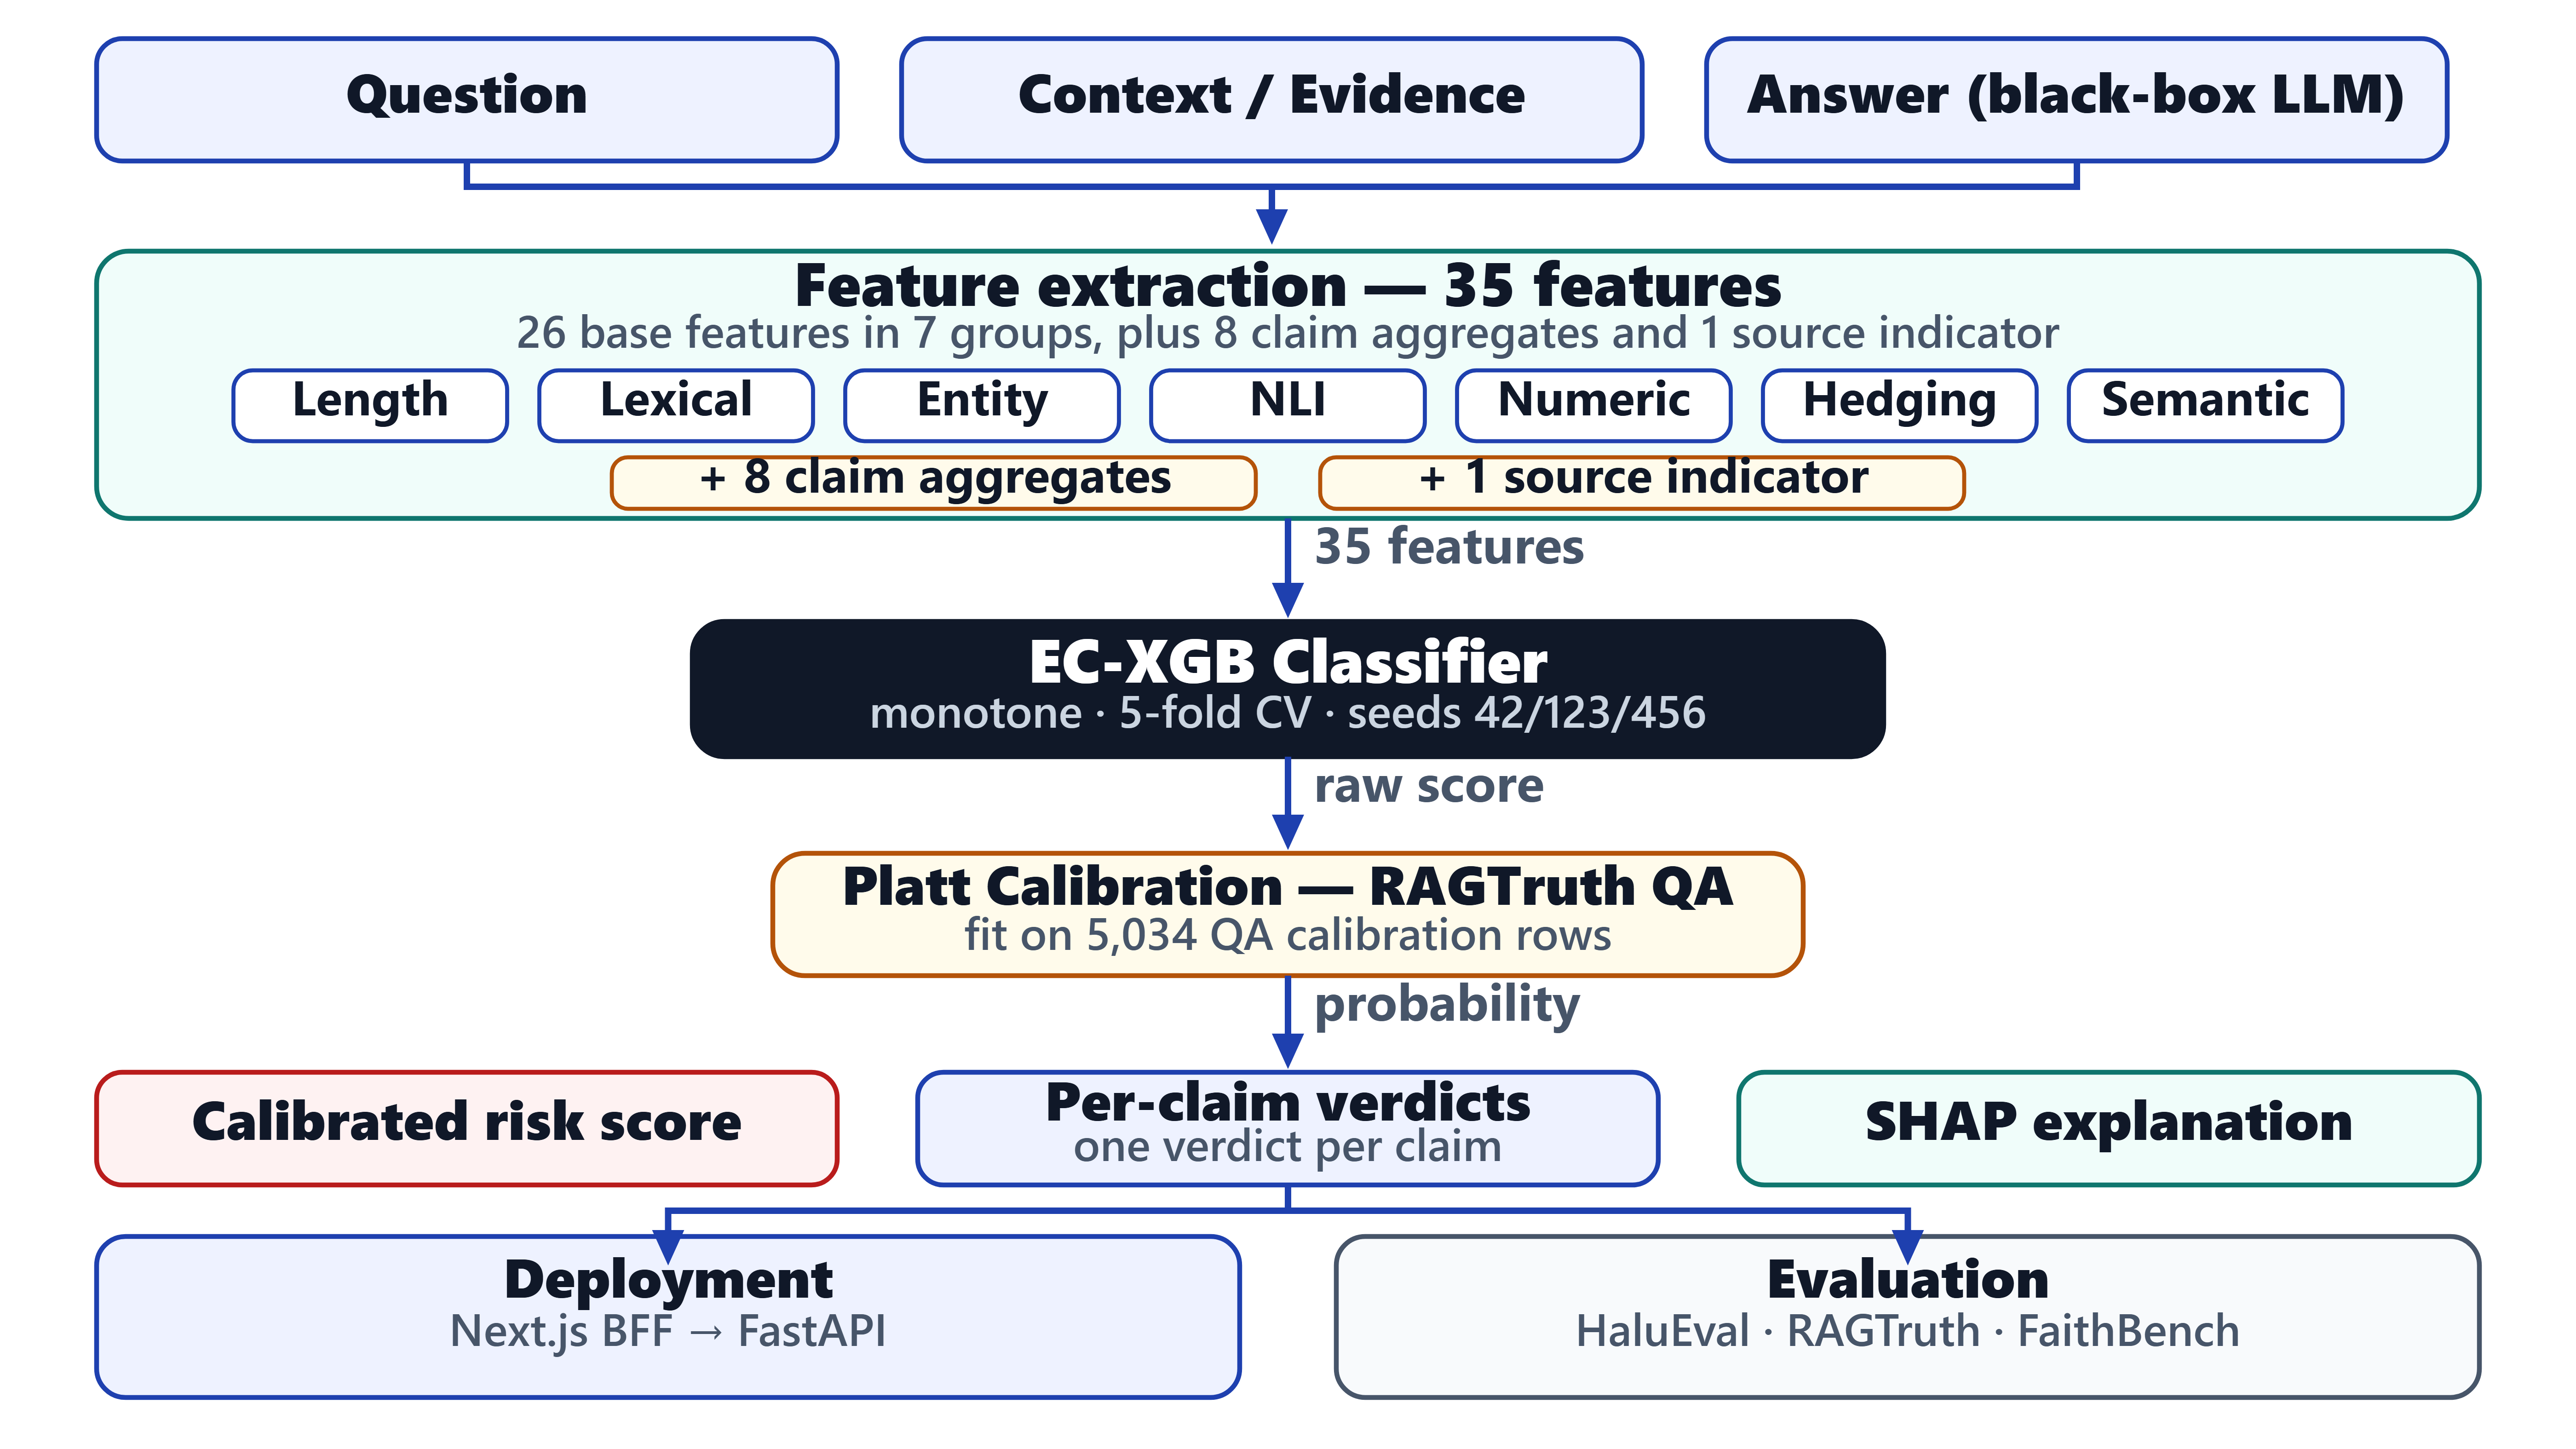
\includegraphics[width=0.98\linewidth]{revision/architecture-flow-large.png}
  \caption{End-to-end pipeline of EC-XGB.}
  \label{fig:pipeline}
\end{figure}

The task is to estimate $P(\text{hallucinated}\mid q,c,a)$ for a question $q$, reference context $c$ (if available), and a candidate answer $a$ from a black-box LLM, in many respects. Figure~\ref{fig:pipeline} is revealing the pipeline that is computing this probability; in fact, the target is not truthfulness in broad but evidence consistency, like whether $a$ follows from $c$ or contradicts it, and the output is a probability that a decision threshold turns into a flag, in many respects. Viewed through this lens, eC-XGB maps the feature vector to a raw score, and a Platt calibrator fitted on the RAGTruth QA calibration rows maps the score to the displayed probability; and thus, this structure takes the three inputs and pulls 35 characteristics - 26 base features in seven groups, eight claim-level NLI combines, and a source indicator. Such an architecture reports the risk score, per-claim verdicts, and SHAP contributions, and the rightmost block is listing the evaluation corpora. HaluEval measures in-domain performance, RAGTruth summarization and data-to-text measure adaptation to task types seen in training, and RAGTruth QA and FaithBench are held out; in fact, the lower band shows the deployment path, such as a Next.js front end calls a FastAPI service that loads the model, calibrator, explainer and feature models at startup.

\subsection{Features}

The model is using 26 base features in seven groups (Table~\ref{tab:features}) and eight claim-level clusters (Table~\ref{tab:claim}), to a significant degree; NLI probabilities come from a DeBERTa-v3 cross-encoder \cite{deberta} trained on SNLI \cite{snli} and MultiNLI \cite{mnli}, semantic similarity employs MiniLM embeddings \cite{sbert,minilm}, to a significant degree. Also, elements come from spaCy named entity recognition (NER) \cite{spacy}; length is encompassed because HaluEval labels longer answers as hallucinated more often, so it is a strong but fragile signal. Lexical overlap captures copying and is the strongest SHAP feature, and yet, it can't detect a fluent paraphrase that is contradicting the proof; semantic similarity catches paraphrase and topic drift that lexical overlap misses. Under these conditions, a correct answer can introduce a new name, a novel item is a valuable warning sign; while Truely; in fact, hedging words are, in fact, weak on their own but separate a careful correct answer from a confident wrong one. A changed number is a typical and easy-to-detect hallucination; the NLI features are the only group that represents logical support rather than surface overlap. The eight claim aggregates are repeating the NLI signals at level of atomic claims, which is the level a reviewer checks; and thus, RAGChecker also applies entailment-based claim metrics \cite{ru2024ragchecker}.

\begin{table}[pos=htbp]
  \centering
  \caption{Base feature groups (26 features total).}
  \label{tab:features}
  \begin{tabular}{>{\raggedright\arraybackslash}p{2.1cm}>{\raggedright\arraybackslash}p{4.6cm}>{\raggedright\arraybackslash}p{4.4cm}}
    \toprule
    \textbf{Group} & \textbf{Features}                                   & \textbf{Source}   \\
    \midrule
    Length/style   & n\_chars, n\_words, n\_sentences, avg\_word\_len    & regex             \\
    Lexical        & overlap vs.\ context \& question, Jaccard $\times$2 & token sets        \\
    Entity         & entity counts, overlap ratio, novel-entity ratio    & spaCy NER         \\
    NLI            & entail/contradict/neutral $\times$ 2 directions     & cross-encoder NLI \\
    Numeric        & number counts, overlap ratio, novel numbers         & regex             \\
    Hedging        & hedge count, hedge density                          & lexicon           \\
    Semantic       & cosine(context,answer), cosine(question,answer)     & MiniLM            \\
    \bottomrule
  \end{tabular}
\end{table}

\begin{table}[pos=htbp]
  \centering
  \caption{Claim-level NLI aggregates (8 features).}
  \label{tab:claim}
  \begin{tabular}{>{\raggedright\arraybackslash}p{2.3cm}>{\raggedright\arraybackslash}p{7.0cm}>{\raggedright\arraybackslash}p{2.9cm}}
    \toprule
    \textbf{Signal} & \textbf{Features}                                                       & \textbf{Source}   \\
    \midrule
    Contradiction   & max and mean contradiction, contradicted-claim ratio                    & NLI cross-encoder \\
    Support         & supported-claim ratio, unsupported-claim ratio, min and mean entailment & NLI cross-encoder \\
    Decomposition   & number of claims                                                        & sentence splitter \\
    \bottomrule
  \end{tabular}
\end{table}

\subsection{Evidence-Consistent XGBoost}

The standard setup is changed by EC-XGB in its feature treatment and its training rows, broadly speaking, and the character and word counts are log-scaled. Also monotone constraints are placed on the evidence features; in fact, the same NLI scorer and support-first rule are applied as the verification layer by them, in many respects. The eight claim features in Table~\ref{tab:claim} are added, like seven NLI aggregates and a claim count; all other attributes are unconstrained. The restrictions are negative on context overlap, context Jaccard, context entailment, context cosine, claim minimum and mean entailment, and the supported-claim ratio, and positive on context contradiction, novel-entity ratio, novel numbers, claim maximum and mean contradiction, and the contradicted-claim ratio; a claim is supported when any kept sentence has an entailment probability of at least 0.5 and at least as high as its contradiction probability, successfully iing contradicted when no sentence supports it. Along these dimensions, also a sentence has, as a practical matter, a contradiction probability of at least 0.5 and above its entailment probability. Otherwise it is unsupported.

Consider an answer with $K$ claims. Let $C(k)$ be the maximum contradiction probability of claim $k$ over its chosen context sentences, $E(k)$ the maximum entailment probability, and $v_k$ its verdict, to a significant degree. The accumulate vector is
\begin{equation}
  \psi(x) = [\max_k C(k), \overline{C}, r_{\text{con}}, r_{\text{sup}}, r_{\text{unsup}}, \min_k E(k), \overline{E}, K],
\end{equation}
with
\begin{equation}
  r_{\text{con}} = \frac{1}{K}\sum_{k=1}^{K} \mathbf{1}[v_k = \text{contradicted}], \quad
  r_{\text{sup}} = \frac{1}{K}\sum_{k=1}^{K} \mathbf{1}[v_k = \text{supported}], \quad
  r_{\text{unsup}} = \frac{1}{K}\sum_{k=1}^{K} \mathbf{1}[v_k = \text{unsupported}].
\end{equation}
Here $x=(q,c,a)$ is the input triplet. Also, $\overline{C}$ and $\overline{E}$ are the means of $C(k)$ and $E(k)$ over the claims, to a significant degree. Within this framework, for $K>0$, the three ratios sum to one. The model input has 35 dimensions, namely the 26 base features (two of them log-scaled), the eight claim features, and one source indicator, in actual application.

The training set adds the RAGTruth summarization and data-to-text rows. The ablation ladder is starting from m0, the 26-characteristic standard reference, and adds log-scaled length counts with monotone constraints at m1, the eight claim features at m2 (34 characteristics), and the RAGTruth non-QA rows with the source indicator at m3 (35 traits). A binary source indicator is one for those rows and zero for HaluEval, so the classifier can separate the two sources. The classifier never sees RAGTruth QA rows, so its QA ranking is zero-shot. The display calibrator does see labeled QA rows below, so the display score is not zero-shot. The 35-feature combination is called EC-XGB. Also, seed 42 is the rolled out checkpoint. Simultaneously, the other seeds are a stability check. Building on this observation, the ablation in Section~\ref{sec:results} is revealing that the claim block adds no accumulate F1 gain. Also, the claim count $K$ is kept because an answer with many claims is harder to corroborate. Algorithm~\ref{alg:ecxgb} is listing the protocol: stages 1 and 2 build the feature matrix, and phases 3 to 9 repeat the fit for the three seeds. Each repetition builds the 35-feature input, trains on HaluEval plus the RAGTruth non-QA rows, fits the display calibrator on the 5{,}034 QA calibration rows, and picks the source and target thresholds.



\begin{algorithm}[H]
  \caption{Evidence-consistent XGBoost (EC-XGB) training and deployment}
  \label{alg:ecxgb}
  \begin{algorithmic}[1]
    \Require HaluEval QA training and validation rows, RAGTruth summarization and data-to-text training rows, RAGTruth QA calibration rows, seeds $\mathcal{S}=\{42,123,456\}$
    \Ensure seed-42 model and display calibrator, source and target thresholds, per-seed metrics
    \State extract the 26 base features and the eight claim features for every row
    \State log-scale the character and word counts, and attach the monotone constraints
    \For{each seed $s \in \mathcal{S}$}
    \State build the 35-feature input, with the source indicator at zero for HaluEval and one for RAGTruth
    \State train XGBoost on the HaluEval rows plus the RAGTruth non-QA rows, and keep every RAGTruth QA row out of classifier training
    \State fit the Platt display calibrator on the RAGTruth QA calibration rows
    \State select the source threshold on the HaluEval validation split
    \State select the target threshold on the QA calibration rows at a 5\% false-positive budget
    \EndFor
    \State \Return the seed-42 model and calibrator, both thresholds, and the per-seed metrics
  \end{algorithmic}
\end{algorithm}



\subsection{Calibration and Explainability}

Source calibration applies the HaluEval validation split, so isotonic regression is fitting a non-decreasing step function $g$ so that $p(x) = g(f(x))$ \cite{isotonic}, in actual application; platt scaling is fitting a sigmoid $p(x) = \sigma(A f(x) + B)$ to the uncalibrated probability $f(x)$, where $A$ and $B$ are fit by maximum likelihood \cite{platt}, in actual application. Under these conditions, both are in comparison to the uncalibrated probability on the HaluEval test split; in turn, the comparison reports anticipated calibration error over 10 equal-width bins,
\begin{equation}
  \mathrm{ECE} = \sum_{m=1}^{M} \frac{|B_m|}{n} \left| \mathrm{acc}(B_m) - \mathrm{conf}(B_m) \right|,
\end{equation}
Post-hoc calibration degrades when the target distribution moves \cite{gasparin2024distance}. where $\mathrm{acc}(B_m)$ and $\mathrm{conf}(B_m)$ are the empirical positive rate and mean confidence in bin $B_m$, the Brier score $\mathrm{BS} = \frac{1}{n}\sum_i (\hat{p}_i - y_i)^2$, and reliability diagrams \cite{guo}, in real-world scenarios.

The second protocol is fitting the calibrator on labeled target rows and gauges it on a disjoint target test split, in actual application. Against this backdrop, the rolled out EC-XGB show score employs a Platt calibrator fitted on the 5{,}034 RAGTruth QA calibration rows; those rows are scored with the source indicator set to one; in turn, also, the API is using the same value for every request; this target calibration needs labeled target rows and is not zero-shot, to a significant degree. The source-only protocol (P0 in Table~\ref{tab:protocols}) is, broadly speaking, fitting both the calibrator and the threshold on the HaluEval validation split; an earlier deployment fit juxtaposed Platt and isotonic on the test split, and Section~\ref{sec:results} entries that choice. The rolled out calibrator is Platt.

Exact SHAP values \cite{shap} are being computed for the raw XGBoost model by a TreeExplainer, in many respects, and also, global importance is the mean absolute SHAP value over a stratified test sample, on the whole. In this broader context, also the five characteristics with the largest absolute value for one prediction are returned by the explanation endpoint. Six operators, including element, number and date replacement, support removal, context insertion, and section shuffling are adopted by a 20-case pilot; it reports the mean absolute score change, the fraction of large changes, the top-1 flip rate, and the Spearman rank correlation between the original and perturbed rankings. Post-hoc attributions can be unstable even when the model is fixed \cite{kelodjou2024shap}, so the pilot gauges them directly \cite{adebayo2018}.

\subsection{System and Reproducibility}

That strategy is rolled out in a web application with a Next.js front end and a FastAPI backend, broadly speaking; indeed, the analyze route calls FastAPI through the \texttt{/api/ml/*} rewrite. The browser calls the Next.js backend-for-frontend (BFF), which streams chat tokens and forwards tool calls to the model, to a significant degree; FastAPI loads the EC-XGB model, the Platt calibrator, the SHAP explainer, and the NLI, spaCy and MiniLM feature models at startup. The rolled out checkpoint is the 35-feature m3 model with seed 42. Section~\ref{sec:results} is comparing it with B2, the standard 26-feature checkpoint tuned on HaluEval QA, and with B6 m0, the fixed-hyperparameter 26-feature reference from the same tuning protocol. Claims are split from the answer and verified with sentence-level NLI against the offered setting, a local passage index, or a web search API; in fact, a claim is, for all practical purposes, supported when any kept sentence has an entailment probability of at least 0.5 and at least as high as its contradiction probability. A contradiction decides only when no sentence supports the claim; in turn, a relevance gate is dropping sentences with no claim vocabulary, and also, the verdicts are revealed per claim. Along these dimensions, the card is following all those verdicts: any contradicted claim sets high risk, another unsupported claim sets medium risk; in fact, also low risk is set by one fully supported answer. The percentage is the display score. The chat card adjusts it by the claim mix, so also, the analyze card reports the unadjusted Platt score. Figure~\ref{fig:pipeline} is showing how one answer is scored; and thus, also Figure~\ref{fig:system} is showing where each constituent runs.

\begin{figure}[pos=htbp]
  \centering
  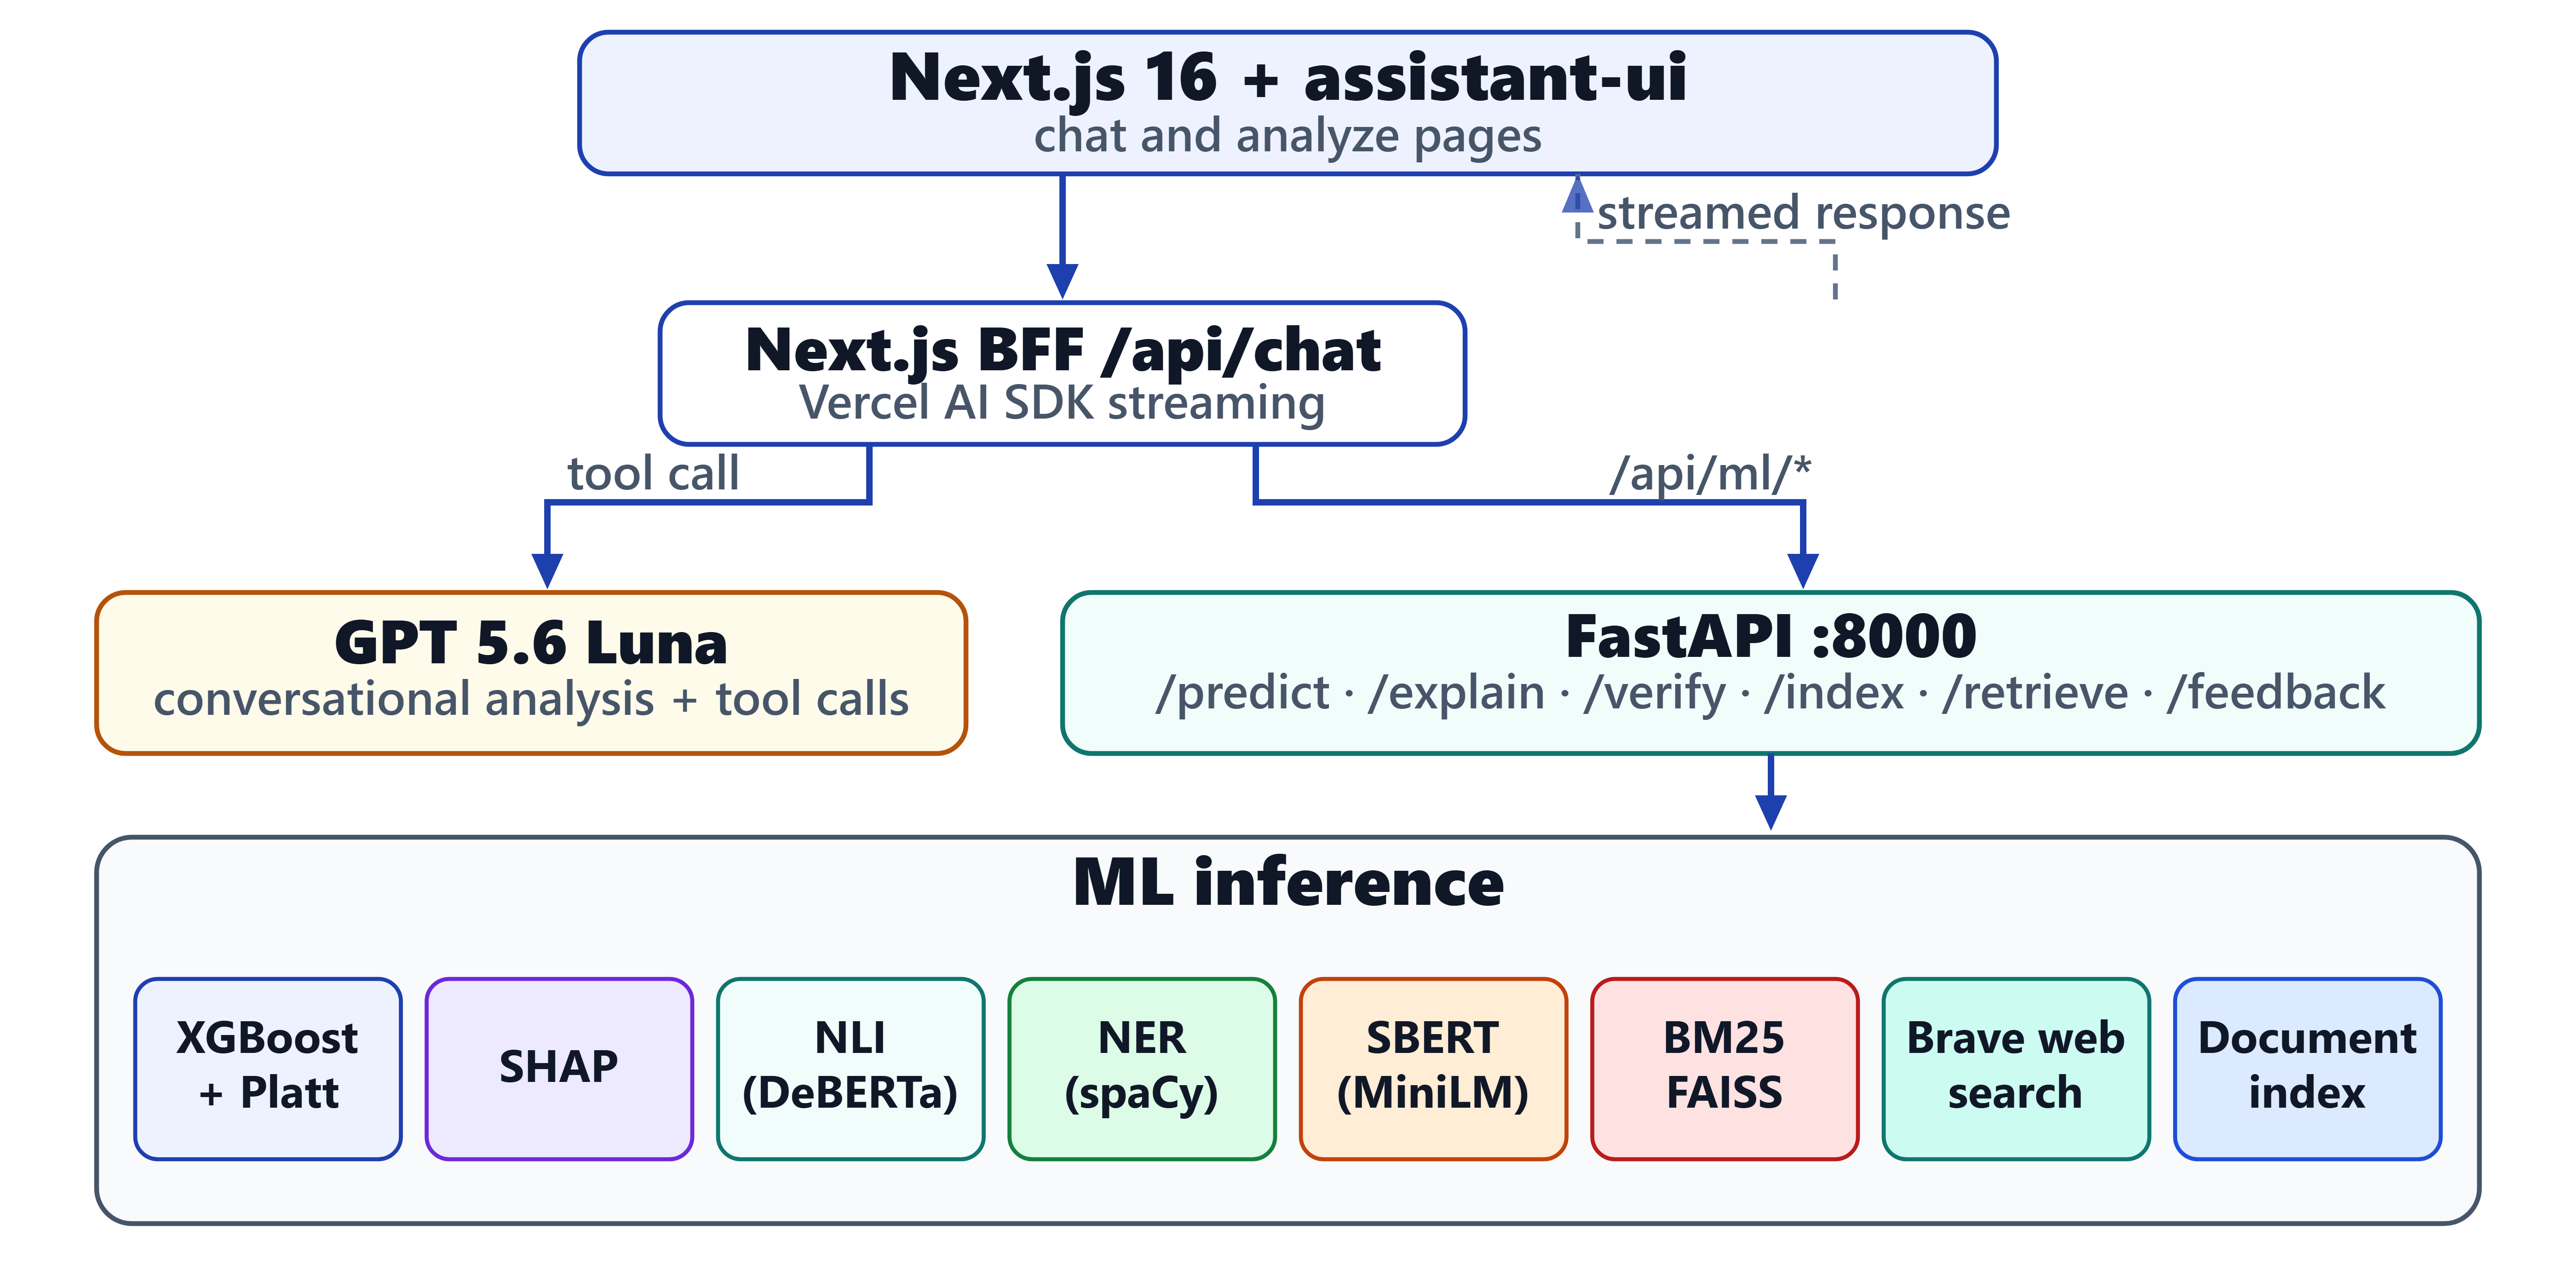
\includegraphics[width=0.98\linewidth]{revision/system-architecture-large.png}
  \caption{Deployment architecture of the HaluRISC system.}
  \label{fig:system}
\end{figure}

5 days per decade are said by the setting, which is why also presumably, the answer is saying 10 in the hallucinated-number case, in real-world scenarios. The raw score is 0.999 and the target-calibrated score is 35.4\%, which the card rounds to 35\% and places in the medium band (0.35--0.60), on the whole. In particular terms, the claim view marks the number claim unsupported, so the chat card also reports medium risk, on the whole. The two labels are agreeing here, but they come from diverse rules. The claim-verdict audit is reliably reported in Section~\ref{sec:results}. The requirements file pins every connection, split indices are, by design, stored with the artifacts, in many respects; also the audit scripts are checking the rebuilt and unchanged reported values against the frozen artifacts, in actual application. The audits run after each build and fail on any mismatch. The insight is the training and evaluation protocol, not a new learner. ECThree standard changes, including log-scaled length counts with monotone constraints, claim-level NLI aggregates for explanation, and multi-source training with the source indicator are principally being combined by -XGB, on the whole. Section~\ref{sec:results} measures what each change contributes. The claim aggregates are kept for per-claim explanation and do not add an combine F1 gain, broadly speaking. The seen-task gain comes from the m3 stack that adds the RAGTruth rows and the source indicator, in real-world scenarios; and thus, also the two are not separated. The risk score needs no LLM judge calls. The optional claim judge is a separate verification step, and also, this reported EC-XGB results do not apply it.

\section{Experiments}\label{sec:experiment}

\subsection{Experimental Setup}

All tests were run on a Windows laptop with an NVIDIA RTX 3060 6\,GB GPU, CUDA 12.8, torch 2.11.0+cu128, and 32\,GB of RAM, in real-world scenarios; seeds 42, 123, and 456 are repeated where a seed employs; the single-seed tables are labeled, in actual application. In light of this dynamic, the code is running on Python 3.12 with scikit-learn 1.9.0, XGBoost 3.3.0, SHAP 0.52.0, spaCy 3.8.14, and sentence-transformers 5.6.1; every seed is tuned separately for the primary comparison, and the component ablation in Section~\ref{sec:results} configures fixed, across the types so that the feature effects are not confounded with tuning. Each run can be reproduced on account of saved split indices and centralized seeds; in turn, a randomized search was effectuated over 30 hyperparameter configurations with grouped five-fold cross-validation, and for the seed-42 standard model, the configuration has a maximum tree depth of 5, a learning rate of 0.05, 300 trees, a subsampling ratio of 0.7, and a column sampling ratio of 0.7.

\subsection{Dataset}

HaluEval QA \cite{haluEval} is offering 10{,}000 question pairs, each with a knowledge passage, a correct answer, and a hallucinated answer, broadly speaking; indeed, HaluEval is completely ChatGPT-generated \cite{haluEval,bang-etal-2025-hallulens}, so the boundary between a factual discrepancy and a hallucination is not always clean, to a significant degree. The split is 70/15/15 by item, so both answers to a question stay together; natural responses with human span annotations are supplied by RAGTruth \cite{ragtruth}, and FaithBench \cite{faithbench} supplies modern-LLM summarization hallucinations. RAGTruth is keeping its official document-level split - summarization and data-to-text supply the training rows and a held-out test set each, and QA supplies 5{,}034 calibration rows and a held-out test set, and RAGTruth QA is a subset of the full corpus, so its rows are not additive. Under these conditions, the three held-out test splits form the pooled RAGTruth test set, so Table~\ref{tab:datasets} is listing the corpora, sizes and positive rates; and thus, MedHallu pqa\_labeled \cite{pandit2025medhallu} adds medical QA pairs with human-annotated gold answers and paired LLM-written hallucinations. HaluBench \cite{ravi2024lynx} contributes a stratified 30\% sample of its DROP, FinanceBench, and covidQA rows, balanced across PASS and FAIL; its HaluEval, RAGTruth, and PubMedQA rows are excluded; a seeded sample from each HaluEval task forms the task-shift sets; in turn, these external corpora are never applied for fitting or threshold selection.

\begin{table}[pos=htbp]
  \centering
  \caption{Datasets used for training and evaluation.}
  \label{tab:datasets}
  \begin{tabular}{lcccc}
    \toprule
    \textbf{Corpus} & \textbf{Rows} & \textbf{Groups} & \textbf{Positive} & \textbf{Use}              \\
    \midrule
    HaluEval QA     & 20{,}000      & 10{,}000        & 50.0\%  & train / validation / test \\
    RAGTruth QA     & 5{,}934       & 989             & 17.8 / 31.1\% & held-out test + calibration  \\
    RAGTruth full   & 17{,}790      & 2{,}965         & 34.9\%  & train + pooled test (2{,}700)     \\
    FaithBench      & 750           & 750             & 68.1\%  & zero-shot                 \\
    MedHallu        & 2{,}000       & 1{,}000 pairs   & 50.0\%  & zero-shot external        \\
    HaluBench subset & 900          & 3 sources       & 50.0\%  & zero-shot external        \\
    HaluEval dialogue & 2{,}000     & 1{,}000 pairs   & 50.0\%  & task-shift test           \\
    HaluEval summarization & 2{,}000 & 1{,}000 pairs & 50.0\%  & task-shift test           \\
    \bottomrule
  \end{tabular}
\end{table}

Guiding and trailing whitespace is trimmed, and lexical matching is case-folded. NER and NLI read the original text. Also entity strings are lowercased for matching. Claims are split into at most six clause-level segments, with conjunctions broken into separate sections, on the whole; in m1 and later versions, the two length counts are log1p-transformed; m0 and the standard model keep raw counts, to a significant degree. Within this framework, a missing setting is a special case, including lexical overlap is 0 and NLI probabilities are homogeneous; and thus, when the setting has more than four sentences, each individual claim is matched to its four best sentences by token overlap. Also, each side of a pair is shortened to 400 characters; in fact, a RAGTruth answer is positive when it carries at least one annotated hallucination span. Both index sets are frozen. FaithBench severity annotations are reduced by a worst-severity rule, and a Questionable annotation counts as positive; and thus, HaluEval applies its native label. NLI and SBERT inference ran on the reference GPU in fp16; also simultaneously, lexical and element attributes run on the CPU. The feature-based logistic baselines standardize their inputs on the training split; the TF-IDF models apply sparse features, and XGBoost does not scale; the source indicator is 1 for FaithBench and MedHallu and 0 for HaluBench and the task-shift sets. FaithBench and RAGTruth summarization and data-to-text have no question; indeed, still question overlap is 0 and question similarity is the cosine between the answer and the encoded empty string. Licenses and the data-availability statement are typically in the Declarations.

\subsection{Baselines and Experimental Procedure}

Twelve models are tested. The heuristic sets risk to one minus lexical overlap, which is why a length-only logistic control is employing the two log-scaled length counts, in actual application. Logistic regression and a 300-tree random forest are, in effect, the standard comparators. To be precise, the 26 base features are applied by the standard XGBoost model \cite{xgboost}, in many respects. Three further controls are isolating the feature design: NLI-only, answer-only TF-IDF, and full-input TF-IDF, to a significant degree. A majority classifier, a fine-tuned RoBERTa-base \cite{liu2019roberta}, and a reduced reimplementation of the lightweight ensemble of Sundaragiri et al.\ \cite{ijert} complete the set; the two judges are in Section~\ref{sec:results}, on the whole. Internal-state detectors are consistently outside the black-box setting \cite{inside2024}. The RoBERTa baseline receives up to 256 tokens and trains for three epochs. The majority baseline anticipates the negative class, so probability metrics are commonly undefined. The external ensemble applies five characteristics (ROUGE-L, SBERT cosine, two NLI probabilities, answer length) in a logistic regression fit on the 14{,}000 training rows, and a validation-selected threshold of 0.55 gives F1 0.9514, in many respects; still, the fixed 0.5 threshold does not change the comparison. EC-XGB's display calibrator is normally fitted on the RAGTruth QA split; the in-domain Platt calibrator is primarily fitted on validation, broadly speaking. Metrics are predominantly reported to four decimals and rates to one. Significance applies McNemar on seed-42 predictions, 2,000 two-level bootstrap resamples, and Wilcoxon across the seeds, in actual application. No question is appearing in both training and check. Calibration is contrasted on raw, Platt, and isotonic scores; Table~\ref{tab:protocols} specifies P0, P1, and P2, and every protocol is using the same test rows, on the whole.

\begin{table}[pos=htbp]
  \centering
  \caption{The three evaluation protocols.}
  \label{tab:protocols}
  \begin{tabular}{lllc}
    \toprule
    \textbf{Protocol}     & \textbf{Calibrator fit}           & \textbf{Threshold fit} & \textbf{Zero-shot} \\
    \midrule
    P0 source-only        & HaluEval validation (3{,}000)     & HaluEval validation    & yes                \\
    P1 target-calibrated  & RAGTruth QA calibration (5{,}034) & fixed at 0.5           & no                 \\
    P2 target-thresholded & RAGTruth QA calibration (5{,}034) & same rows at 5\% FPR   & no                 \\
    \bottomrule
  \end{tabular}
\end{table}

P1 is applied by the rolled out framework; also p2 is the thresholded alternative. SHAP \cite{shap} TreeExplainers globally are explaining. Feature latency is, in effect, measured on 200 HaluEval rows on the reference laptop. Two checks test reliability - the rank agreement between the m3 and B2 SHAP importances and a six-operator perturbation pilot, to a significant degree; Only P0 is zero-shot; P1 and P2 read labels from the target calibration split, which is disjoint from the test split, broadly speaking. Against this backdrop, the 900 RAGTruth QA rows are scored by two judges, GPT-5.6 Luna and Qwen 3.5 4B, under the LLM-as-a-judge protocol \cite{zheng2023judge}, and also, costs are computed from the recorded token counts.

\subsection{Evaluation Metrics}

Two families of metrics are reported. Building on this observation, TP and TN are true positives and true negatives; precision is the share of flagged answers that are truly hallucinated. The false-positive rate (FPR) is the share of correct answers that are flagged, which is the operating constraint, under the distribution shift, to a significant degree; indeed, recall is the share of hallucinated answers that the detector catches, and F1 is their harmonic mean, in real-world scenarios. Both are needed because a model can (in practice) rank well and still make poor decisions when the threshold is fixed; in fact, threshold-dependent metrics measure the decision at a fixed cut-off, and threshold-free metrics measure how well a model ranks answers. In the interim, FP and FN are false positives and false negatives, such as a correct answer flagged as hallucinated, and a hallucinated answer that is not flagged; the flag rate is the share of answers above the decision threshold; in turn, also, a rate near 100\% means every answer is reaching a human reviewer.
\begin{gather}
  \text{Precision }(P) = \frac{\mathrm{TP}}{\mathrm{TP} + \mathrm{FP}}, \qquad
  \text{Recall }(R) = \frac{\mathrm{TP}}{\mathrm{TP} + \mathrm{FN}}, \qquad
  F_1 = \frac{2PR}{P+R}, \\
  \text{False-positive rate }(\mathrm{FPR}) = \frac{\mathrm{FP}}{\mathrm{FP} + \mathrm{TN}}, \qquad
  \text{Flag rate} = \frac{1}{n}\sum_{i=1}^{n}\mathbf{1}[\hat{p}_i \ge \tau].
\end{gather}

The second group measures ranking, calibration and paired error patterns; in fact, AUROC is the probability that a randomly chosen hallucinated answer receives a higher score than a randomly chosen correct answer, with 0.5 at chance, in real-world scenarios. All four cells of the confusion matrix are applied by the Matthews correlation coefficient (MCC) and ranges from $-1$ to $1$, with zero at chance, in many respects; and thus, the subfield under the precision-recall curve (PR-AUC) is more sensitive than AUROC when the positive class is rare. Building on this observation, rAGTruth QA has a positive rate of 17.8\%, so PR-AUC is reported beside AUROC; the Wilson interval is giving a 95\% range for a proportion and is applied for the P2 recall and false-positive rate, where the counts are small.
\begin{gather}
  \mathrm{AUROC} = \int_{0}^{1} \mathrm{TPR}(u)\, d\,\mathrm{FPR}(u) = P(s^{+} > s^{-}), \\
  \mathrm{PR\text{-}AUC} = \int_{0}^{1} P(r)\, dr, \qquad
  \mathrm{MCC} = \frac{\mathrm{TP}\cdot\mathrm{TN} - \mathrm{FP}\cdot\mathrm{FN}}{\sqrt{(\mathrm{TP}+\mathrm{FP})(\mathrm{TP}+\mathrm{FN})(\mathrm{TN}+\mathrm{FP})(\mathrm{TN}+\mathrm{FN})}}, \\
  \mathrm{CI}_{95\%} = \frac{\hat{p} + \frac{z^2}{2n} \pm z\sqrt{\frac{\hat{p}(1-\hat{p})}{n} + \frac{z^2}{4n^2}}}{1 + \frac{z^2}{n}}.
\end{gather}

\section{Results}\label{sec:results}

\subsection{Model Comparison}

Table~\ref{tab:models} reports the HaluEval test results for eleven baselines and EC-XGB, averaged over three seeds where a seed applies, on the whole; indeed, the diminished external ensemble is below EC-XGB by 0.0337 F1 [0.0262, 0.0419] and 0.0135 AUROC [0.0098, 0.0177]; it is trained on fewer rows and with a narrower feature set, so that gap is descriptive, in actual application. Simultaneously, answer-only TF-IDF is much stronger, so adding the question and context hurts. Against this backdrop, the weak controls are NLI-only and full-input TF-IDF; the ranking columns are repeating that pattern, namely EC-XGB is first among the feature-based models on AUROC and PR-AUC, the established model and random forest are close behind, and RoBERTa is slightly higher. Calibration is giving a distinct summary, because the standard model has the lowest ECE while EC-XGB and RoBERTa more lowly score. Still, the benchmark does not settle the ordering; and thus, EC-XGB is directing the classic model by 0.0009 F1, which is smaller than the width of the conventional seed-42 bootstrap interval [0.9812, 0.9895]. Figure~\ref{fig:rocpr} is revealing the curves behind the table; and thus, also; while the table values are three-seed means, the curves are using seed 42.

The XGBoost margin over the random forest is 0.0004 F1, with McNemar $p=0.502$; the difference is not major, in many respects; the margin over logistic regression is 0.0187 F1 ($p=1.86\times10^{-10}$) and over the heuristic 0.0495 ($p=2.28\times10^{-30}$), to a significant degree. In parallel with this, one further source-only encoder wins in-domain (F1 0.9912 vs 0.9855) but is near chance on each individual RAGTruth task (AUROC 0.458 on summarization and 0.491 on data-to-text, against 0.736 and 0.770 for EC-XGB on all the tasks); pooling is giving 0.337 for this encoder and 0.582 for EC-XGB, because the encoder's pooled score mixes between-task score shifts with within-task ranking. Any modified encoder on the same multi-source rows is reaching 0.694 on the pooled RAGTruth test set, above EC-XGB's 0.582, so the seen-task gain is not precise to the feature model; neither model generalizes to unseen QA (0.490 vs 0.549). Also faithBench is worse for both (0.434 vs 0.594); indeed, adaptation helps any model on seen tasks; the feature model is, indeed, keeping its relative ordering on unseen tasks.


\begin{table}[pos=htbp]
  \centering
  \caption{Test-set performance on HaluEval QA, mean over seeds 42/123/456 where a seed applies; deterministic rows are single fits (n = 3{,}000).}
  \label{tab:models}
  \begin{tabular}{lrrrrrrrr}
    \toprule
    \textbf{Model}          & \textbf{P} & \textbf{R} & \textbf{F1} & \textbf{AUROC} & \textbf{PR-AUC} & \textbf{MCC} & \textbf{ECE} & \textbf{Brier} \\
    \midrule
    Heuristic (1$-$overlap) & 0.9473     & 0.9233     & 0.9352      & 0.9132         & 0.8196          & 0.8723       & 0.3541       & 0.2672         \\
    Length-only (2 feats)   & 0.9454     & 0.9460     & 0.9457      & 0.9759         & 0.9722          & 0.8913       & ---          & ---            \\
    Logistic regression     & 0.9768     & 0.9553     & 0.9660      & 0.9932         & 0.9901          & 0.9329       & 0.0099       & 0.0253         \\
    Random forest           & 0.9897     & 0.9789     & 0.9842      & 0.9980         & 0.9983          & 0.9687       & 0.0143       & 0.0127         \\
    NLI-only                & 0.6479     & 0.6967     & 0.6714      & 0.7177         & 0.7531          & 0.3189       & 0.0678       & 0.2182         \\
    TF-IDF (answer-only)    & 0.9550     & 0.8920     & 0.9224      & 0.9696         & 0.9665          & 0.8519       & 0.0831       & 0.0662         \\
    TF-IDF (full input)     & 0.6397     & 0.5647     & 0.5999      & 0.6754         & 0.6785          & 0.2484       & 0.0679       & 0.2328         \\
    External ensemble$^\dagger$ & 0.9508 & 0.9527     & 0.9517      & 0.9850         & 0.9856          & 0.9033       & 0.0141       & 0.0391         \\
    XGBoost (conventional)  & 0.9932     & 0.9762     & 0.9846      & 0.9979         & 0.9983          & 0.9697       & 0.0045       & 0.0117         \\
    EC-XGB (m3)             & 0.9939     & 0.9773     & 0.9855      & 0.9984         & 0.9987          & 0.9715       & 0.0074       & 0.0108         \\
    RoBERTa-base            & 0.9955     & 0.9869     & 0.9912      & 0.9990         & 0.9993          & 0.9825       & 0.0070       & 0.0081         \\
    Majority (negative)     & 0.0000     & 0.0000     & 0.0000      & ---            & ---             & 0.0000       & ---          & ---            \\
    \bottomrule
  \end{tabular}
\end{table}



\begin{figure}[pos=htbp]
  \centering
  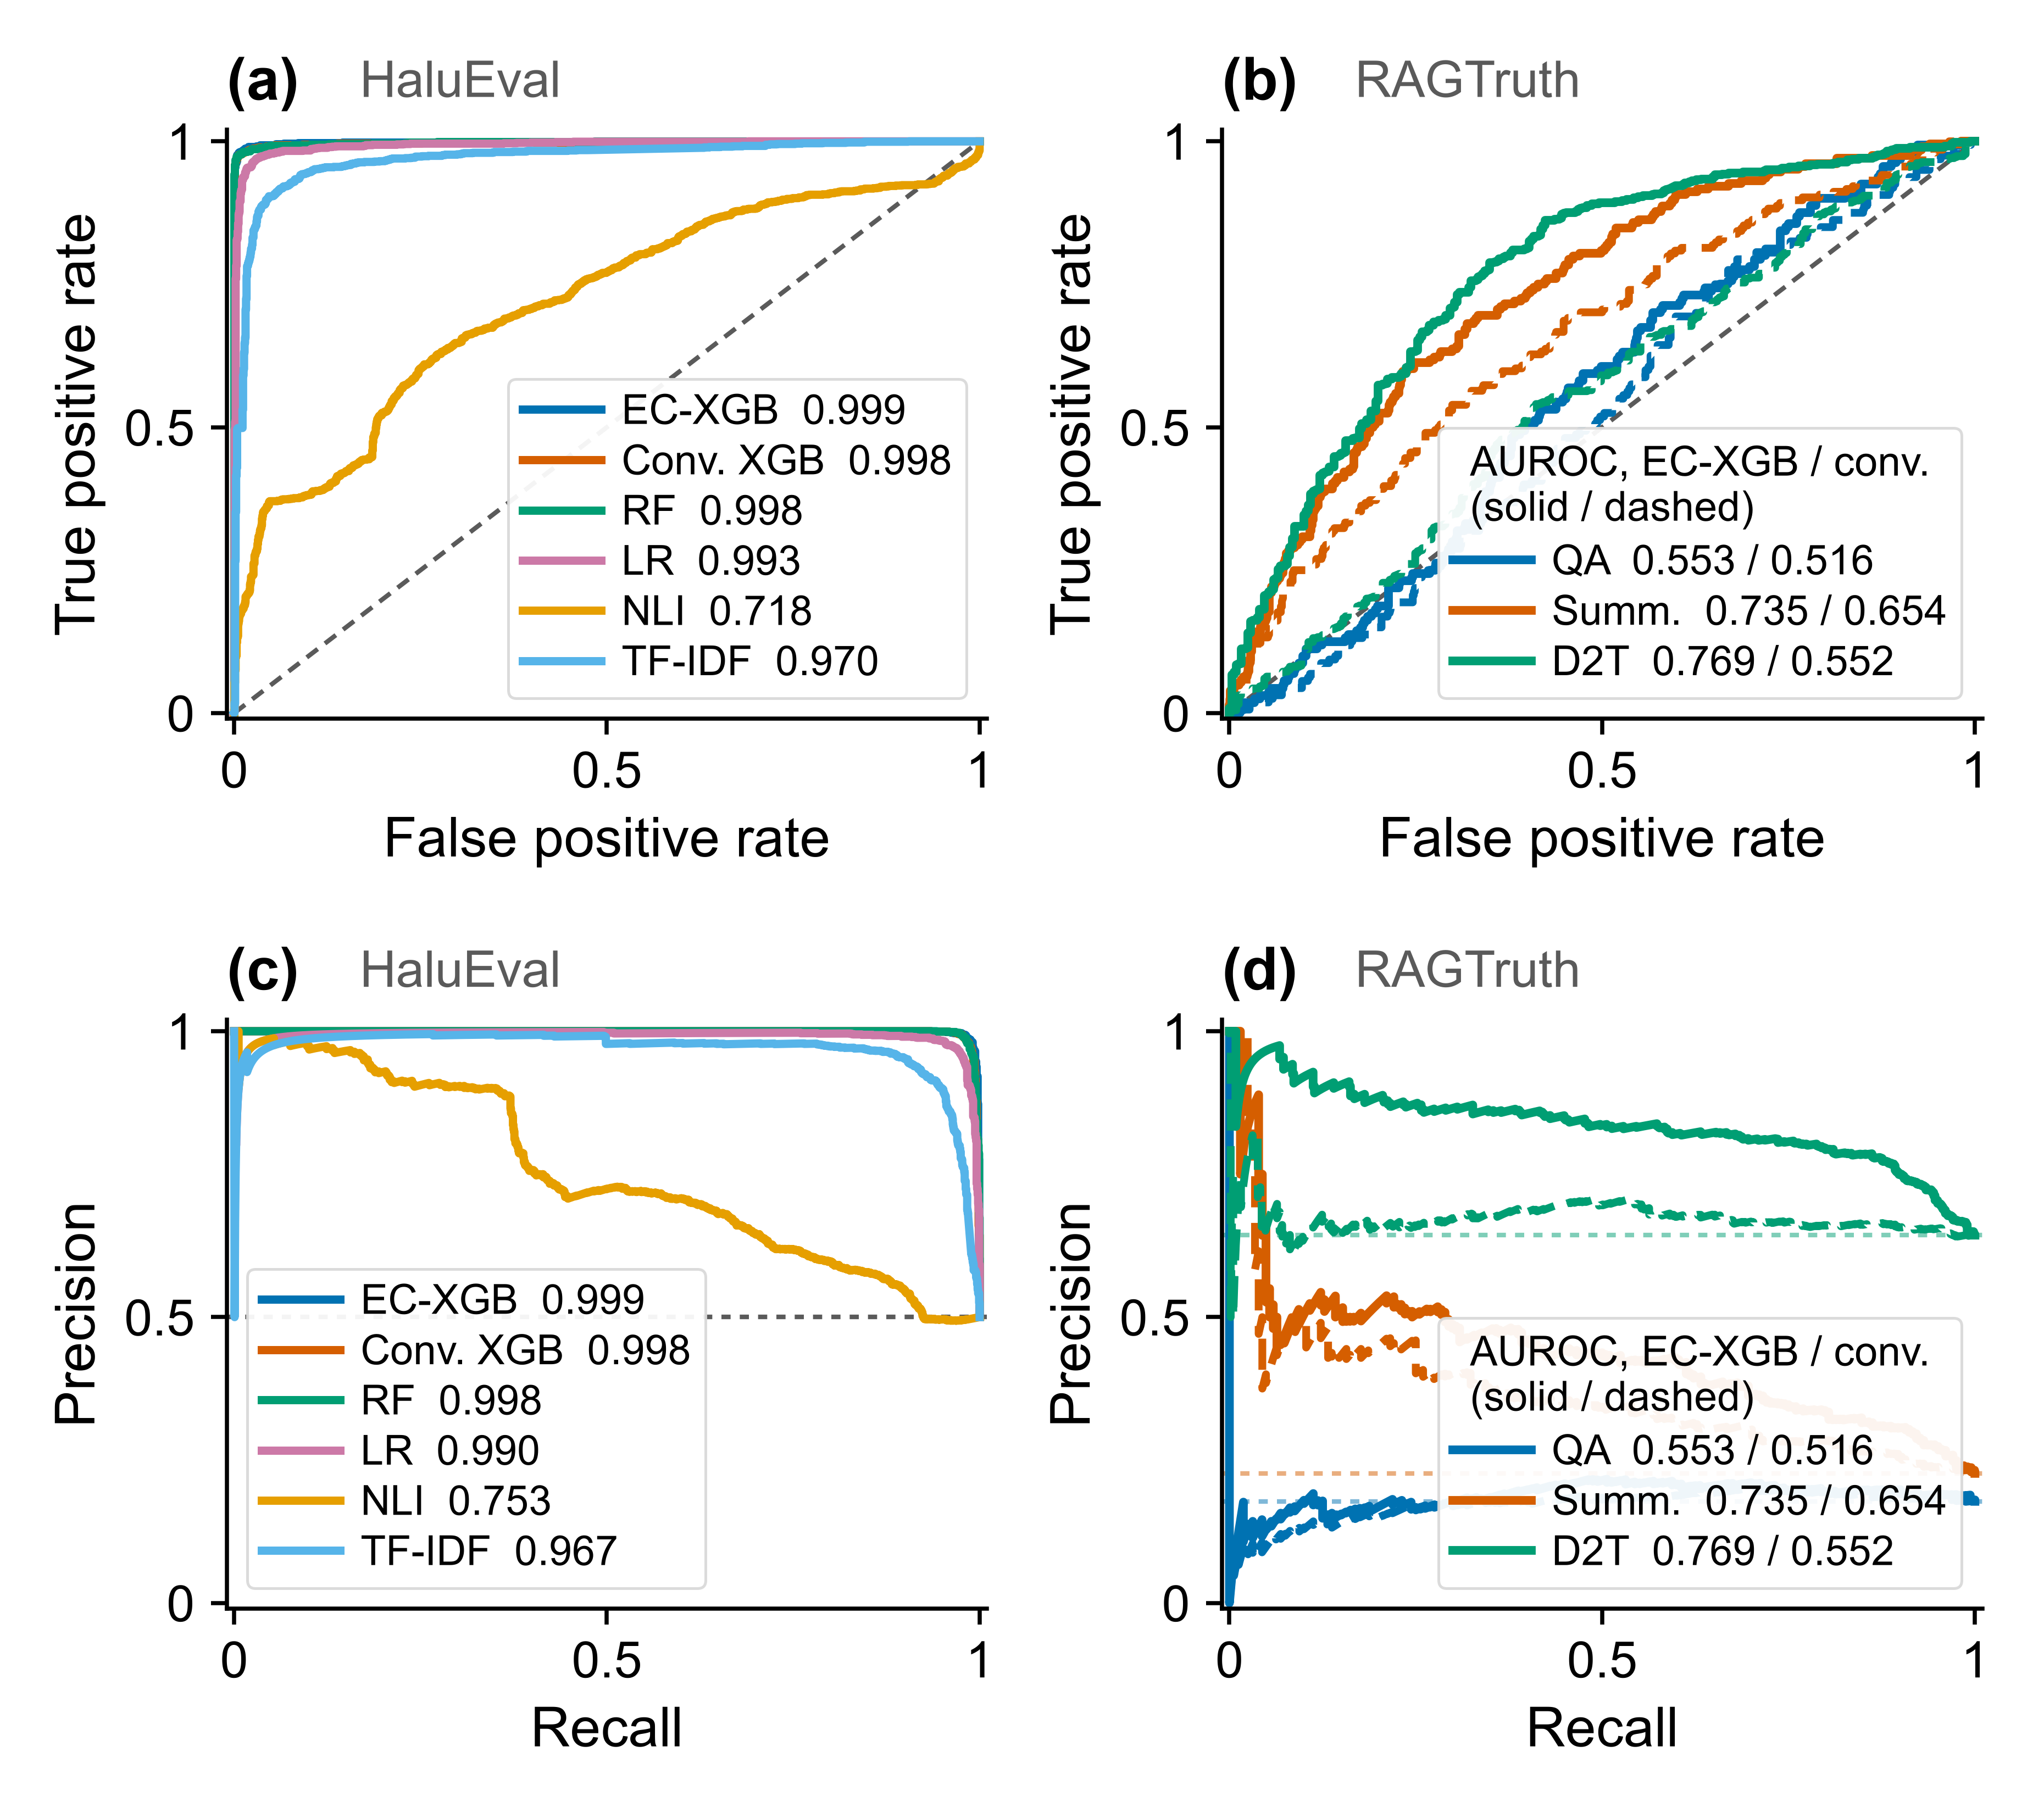
\includegraphics[width=\linewidth]{revision/roc_pr_curves.png}
  \caption{ROC and precision-recall curves on HaluEval and RAGTruth (seed 42).}
  \label{fig:rocpr}
\end{figure}



\subsection{EC-XGB and Ablation}

Table~\ref{tab:ec} reports the component ablation under one fixed-hyperparameter configuration (max depth 5, learning rate 0.05, 300 trees, subsample 0.7, colsample 0.7, chosen once on the m3 seed-42 run), so the columns measure feature effects rather than tuning effects, in actual application; indeed, the gain is not from the claim attributes; it is appearing when the multi-source rows and source indicator are added, on the whole. McNemar is giving $p=0.789$ for m0 vs m3, so the ablation does not solve a difference; the MedHallu source-zero check is proposing the indicator is not the principal driver, but a seen-task source ablation would settle it. The claim clusters change F1 by $-$0.0004 at m2 relative to m1, and the full m3 stack changes it by $+$0.0001; neither is an accumulate gain; and thus, the in-domain F1 span is only 0.0006 across m0--m3. Viewed through this lens, the ladder from m0 to m3 is specified in Section~\ref{sec:proposed}, and ECE is computed on the raw score, and on the pooled RAGTruth split, AUROC rises from 0.494 to 0.590 and raw ECE falls from 0.635 to 0.275; on held-out QA the comparison is 0.556 vs 0.558, within the seed noise. The rolled out checkpoint is reaching 0.9855, under its own tuned configuration, 0.0001 above the fixed ablation.

\begin{table}[pos=htbp]
  \centering
  \caption{EC-XGB component ablation on the HaluEval test set with one fixed configuration, mean over three seeds.}
  \label{tab:ec}
  \begin{tabular}{lccccccc}
    \toprule
    \textbf{Variant} & \textbf{Features} & \textbf{F1} & \textbf{AUROC} & \textbf{MCC} & \textbf{ECE} & \textbf{RAGTruth AUROC} & \textbf{RAGTruth ECE} \\
    \midrule
    m0 conventional  & 26                & 0.9849      & 0.9979         & 0.9701       & 0.0050       & 0.4937                  & 0.6352                \\
    m1 debias        & 26                & 0.9853      & 0.9976         & 0.9710       & 0.0042       & 0.5567                  & 0.6260                \\
    m2 + claims      & 34                & 0.9849      & 0.9985         & 0.9701       & 0.0051       & 0.5461                  & 0.6359                \\
    EC-XGB (m3)      & 35                & 0.9854      & 0.9986         & 0.9713       & 0.0078       & 0.5898                  & 0.2746                \\
    \bottomrule
  \end{tabular}
\end{table}

\begin{table}[H]
  \centering
  \caption{Feature-group ablation of the fixed-hp m3 model on the HaluEval test set, mean over seeds 42/123/456.}
  \label{tab:ablation}
  \begin{tabular}{lrrrr}
    \toprule
    \textbf{Removed group} & \textbf{Features} & \textbf{$\Delta$F1} & \textbf{$\Delta$AUROC} & \textbf{$\Delta$MCC} \\
    \midrule
    length                 & 4 & $-$0.0066 & $-$0.0012 & $-$0.0127 \\
    lexical                & 4 & $-$0.0171 & $-$0.0040 & $-$0.0343 \\
    entity                 & 4 & $-$0.0010 & $+$0.0000 & $-$0.0020 \\
    nli                    & 6 & $-$0.0040 & $-$0.0004 & $-$0.0080 \\
    numeric                & 4 & $-$0.0003 & $+$0.0001 & $-$0.0007 \\
    hedging                & 2 & $+$0.0000 & $+$0.0001 & 0.0000 \\
    semantic               & 2 & 0.0000 & $+$0.0002 & $+$0.0000 \\
    claims                 & 8 & $-$0.0010 & $-$0.0003 & $-$0.0020 \\
    source                 & 1 & $-$0.0001 & $+$0.0001 & $-$0.0002 \\
    \bottomrule
  \end{tabular}
\end{table}

Table~\ref{tab:ablation} repeats the ablation on the fixed-hp m3 model, whose full reference is reaching F1 0.9861, AUROC 0.9985, and MCC 0.9726, broadly speaking; indeed, the claim block costs about one seed standard departure, so an aggregate claim gain is not settled, on the whole. Viewed through this lens, lexical overlap is the largest contributor, followed by length and NLI; in turn, item, numeric, hedging, semantic, and source each change F1 by sub-threshold to 0.0011; and thus, lexical overlap and length therefore carry the in-domain score, which is why also, the remaining groups add ranking information without moving F1 far. Deltas are relative to the full m3 refit under the same configuration, trained on the same 24{,}056 rows and appraised once on 3{,}000 test rows without tuning or early stopping; the refit reference differs from Table~\ref{tab:ec} by 0.0007 F1, within its seed standard deviation of 0.0010.

Figure~\ref{fig:perseed} reveals the seed-level spread behind Table~\ref{tab:ec}. Across seeds, the ECE panel is noisier, like m0 is stable; indeed, the F1 and AUROC panels are tight, with within-variant differences below 0.0007 F1 and 0.0005 AUROC, to a significant degree. Simultaneously, m2 and m3 are deviating more. Taken together, the mean ordering is m3 $>$ m1 $>$ m2 $>$ m0, yet the per-seed ranks flip and the differences are, in practice, below seed noise. The ECE sign is stable: m0 is lower than m3 on every seed, so the ablation does not establish a calibration advantage for m3 in this sample, in actual application.



\begin{figure}[pos=htbp]
  \centering
  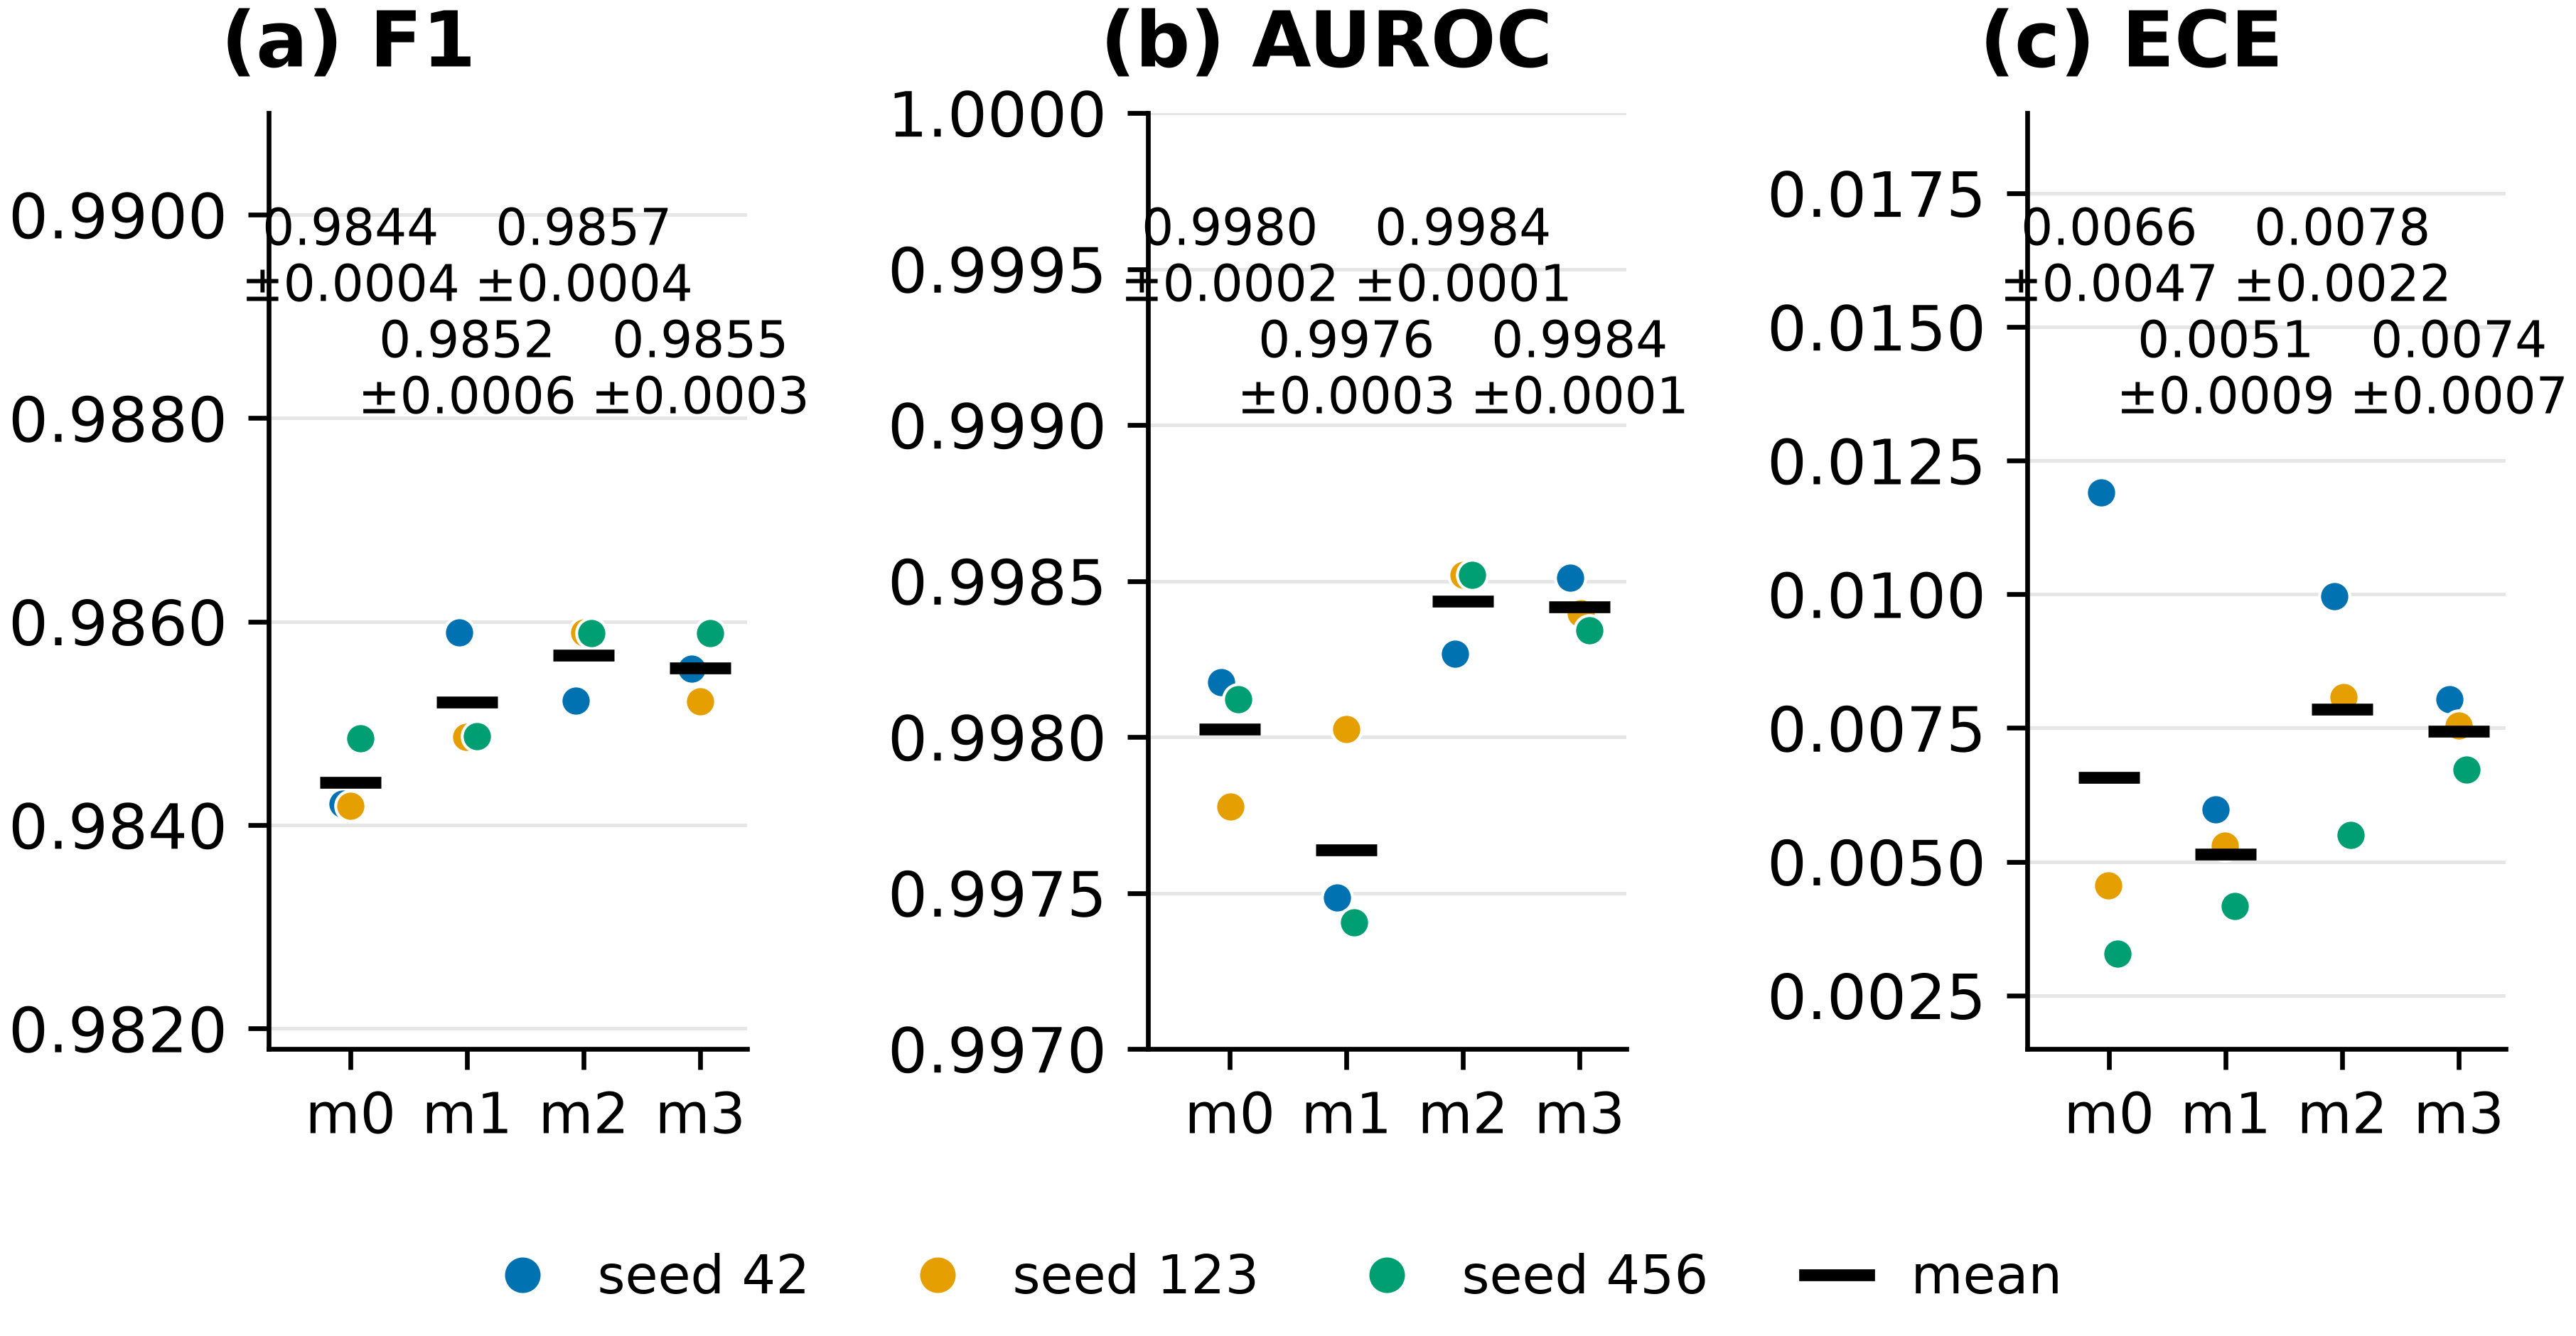
\includegraphics[width=\linewidth]{revision/per_seed_stability.png}
  \caption{Per-seed F1, AUROC and ECE for the fixed-hyperparameter B6 variants.}
  \label{fig:perseed}
\end{figure}



\subsection{Calibration, Shift, and External Validity}

The raw, Platt-scaled, and isotonic versions of the standard model give ECE 0.0045, 0.0091, and 0.0070 on HaluEval, so the optimized ECEs are not lower in this sample, broadly speaking. Figure~\ref{fig:reliability} is revealing why. On HaluEval, the points at the two ends sit on the diagonal; the middle of the score range fewly values, so the curve stably bins, broadly speaking; FaithBench is combined because its scores concentrate near 1.0. Building on this observation, the raw curve is overlaped at both ends by the Platt and isotonic curves; and thus, the m3 raw score is also well adjusted in-domain, with ECE 0.0078, so there is little room for calibration to raise on HaluEval. Platt scaling is fitting a two-parameter logistic map from the uncalibrated probability $s$, called the raw score in the figures, to a probability,
\begin{equation}
  \hat{p} = \sigma(a s + b), \qquad \sigma(z) = \frac{1}{1+e^{-z}},
  \label{eq:platt}
\end{equation}
where $a$ is the calibration slope. Under these conditions, also, $b$ is the intercept, which is why a slope below one means the raw score is substantially overconfident, in actual application; indeed, also a slope near one means the scale is already usable. The aligned score with a constant predictor at the evaluation prevalence is being compared by the Brier skill score (BSS),
\begin{equation}
  \mathrm{BSS} = 1 - \frac{\mathrm{BS}}{\mathrm{BS}_{\mathrm{prior}}}.
  \label{eq:bss}
\end{equation}
A positive BSS means the score beats the prior; a non-positive BSS means it does not.

\begin{figure}[pos=htbp]
  \centering
  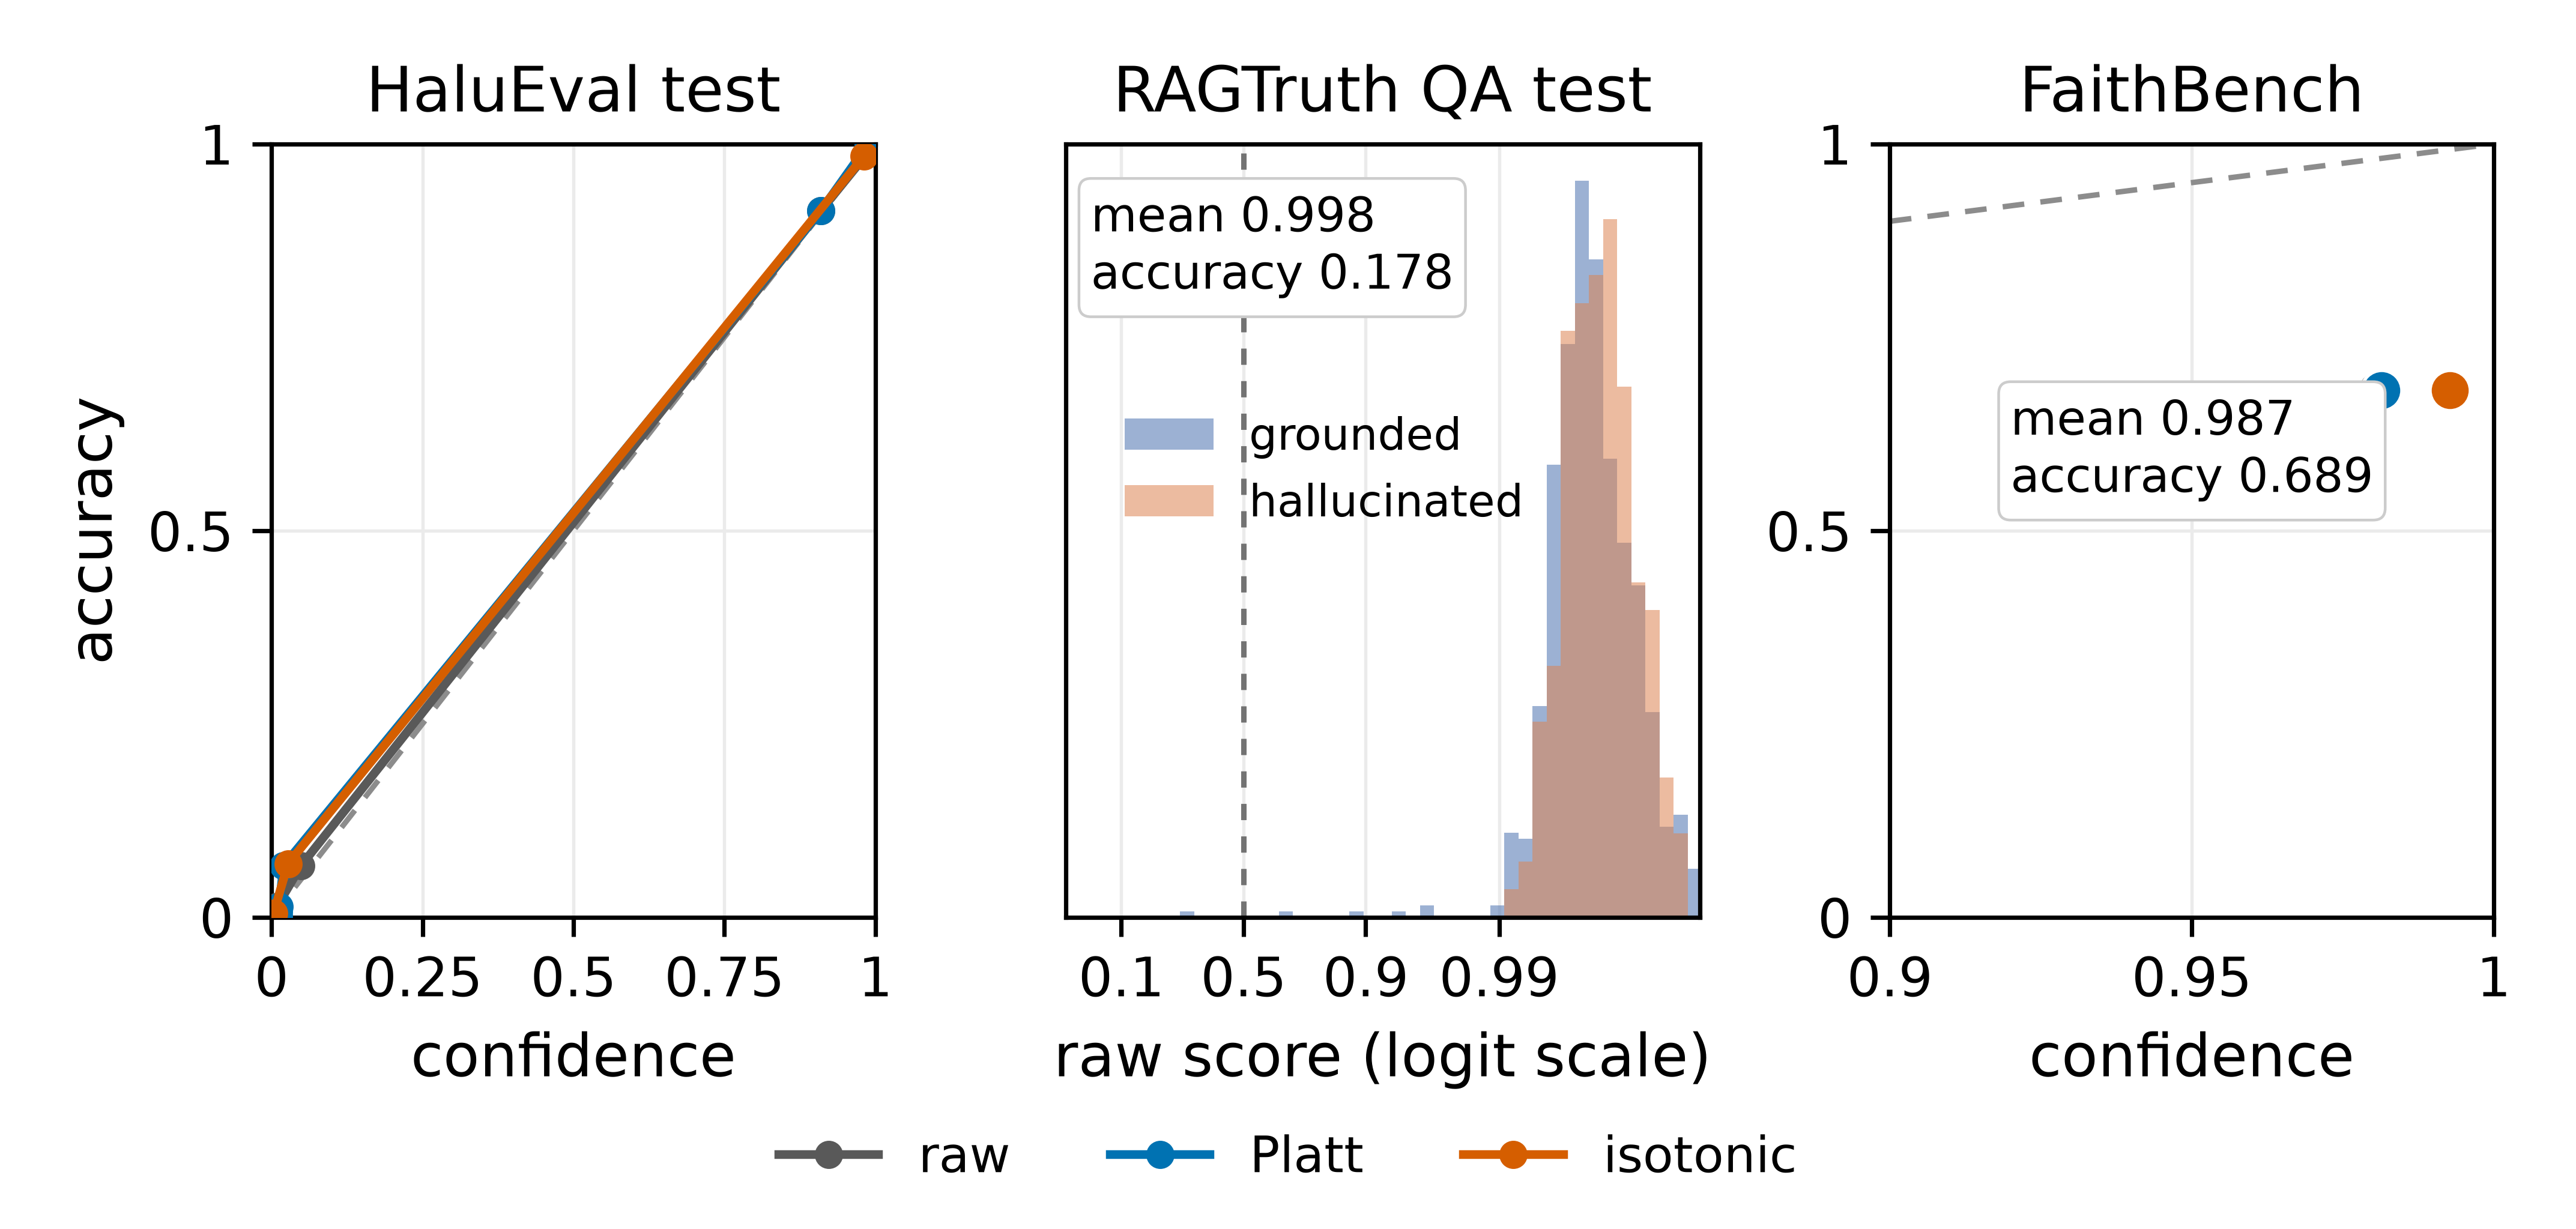
\includegraphics[width=\linewidth]{b4/reliability_diagrams.png}
  \caption{Reliability diagrams for the B2 model on HaluEval and FaithBench, and the RAGTruth QA raw-score distribution.}
  \label{fig:reliability}
\end{figure}

Source Platt can't repair the base-rate shift. Both models on the same test set are reported by Table~\ref{tab:target}. On the HaluEval validation split at a 5\% false-positive budget, the threshold is picked by the source-only operating point (P0), in real-world scenarios. Figure~\ref{fig:calibshift} is revealing the raw and target-recalibrated scores. The standard target-Platt row behaves the same way at ECE 0.134 and Brier 0.164, in real-world scenarios. Calibration fixes the scale, not the ranking; AUROC stays at 0.558. The fixed-hp m3 raw score is severely overconfident on RAGTruth QA, namely ECE 0.731 and Brier 0.689, with a Cox slope of 0.18 on the 5{,}034 calibration rows. Recall is 99.0--99.5\% and FPR stays near 5\% on HaluEval test, but on RAGTruth QA the same threshold flags all 900 rows of the rolled out seed-42 checkpoint, because every score exceeds 0.095, so P0 is not usable. In light of this dynamic, eCE is lowered to 0.125 and Brier to 0.161 by Target Platt, but the Brier skill score against the test prior is $-$0.10, and a constant predictor at the test prevalence has Brier 0.146, lower than every adjusted row. A prevalence-only predictor at 0.1778 reaches ECE 0.000 and Brier 0.146 and projects no positives; at the calibration prevalence of 0.3107 it is giving ECE 0.133 and Brier 0.164, so the calibrator is setting the level to the calibration prevalence and the residual ECE is dominated by the prevalence gap. The standard target-thresholded mode (P2) chooses 0.313 at a 5\% false-positive budget and reaches 5.0\% recall at 5.8\% FPR (precision 15.7\%, F1 0.076). Random flagging at 5.8\% FPR yields 5.8\% recall at 17.8\% prevalence, so P2 is chance-level. At 0.5, P1 flags no RAGTruth QA rows; for the rolled out seed-42 calibrator, the maximum target-Platt score is 0.355 (35.4\% before rounding, 35\% on the card), the median is 0.331, and 16\% of QA rows reach 0.35, so the card typically depends on the per-claim verdict adjustment. Figure~\ref{fig:operating} is showing the operating point and label budget, like mean ECE is 0.130 at 50 rows, 0.124 at 252 rows, and 0.125 at 5{,}034 rows, but a single 252-row draw can miss the full-split ECE by about 0.06. All calibration metrics refer to the pre-verdict score; the displayed percentage is a design aid, not a verified probability.

\begin{table}[pos=htbp]
  \centering
  \caption{Calibration of the fixed-hp m3 model and the conventional target-Platt reference on the RAGTruth QA test set (n = 900, 17.8\% positive). $^{\ast}$Slope: three-seed mean; bracket: envelope of the three per-seed 95\% intervals, not a pooled interval.}
  \label{tab:target}
  \begin{tabular}{llrrrrr}
    \toprule
    \textbf{Predictor} & \textbf{Fit} & \textbf{ECE} & \textbf{Brier} & \textbf{BSS} & \textbf{Slope} & \textbf{Flagged} \\
    \midrule
    Prior (test prevalence) & constant 0.1778 & 0.000 & 0.146 & 0.000 & --- & 0.0\% \\
    Prior (cal prevalence)  & constant 0.3107 & 0.133 & 0.164 & $-$0.12 & --- & 0.0\% \\
    \midrule
    m3 raw          & none            & 0.731 & 0.689 & $-$3.71 & 0.18 [0.12, 0.27]$^{\ast}$ & 96.8\% \\
    m3 source Platt & HaluEval val    & 0.765 & 0.742 & $-$4.07 & --- & 96.8\% \\
    m3 target Platt & RAGTruth cal    & 0.125 & 0.161 & $-$0.10 & --- & 0.0\% \\
    Conventional target Platt & RAGTruth cal & 0.134 & 0.164 & $-$0.12 & --- & 0.0\% \\
    \bottomrule
  \end{tabular}
\end{table}

\begin{figure}[pos=htbp]
  \centering
  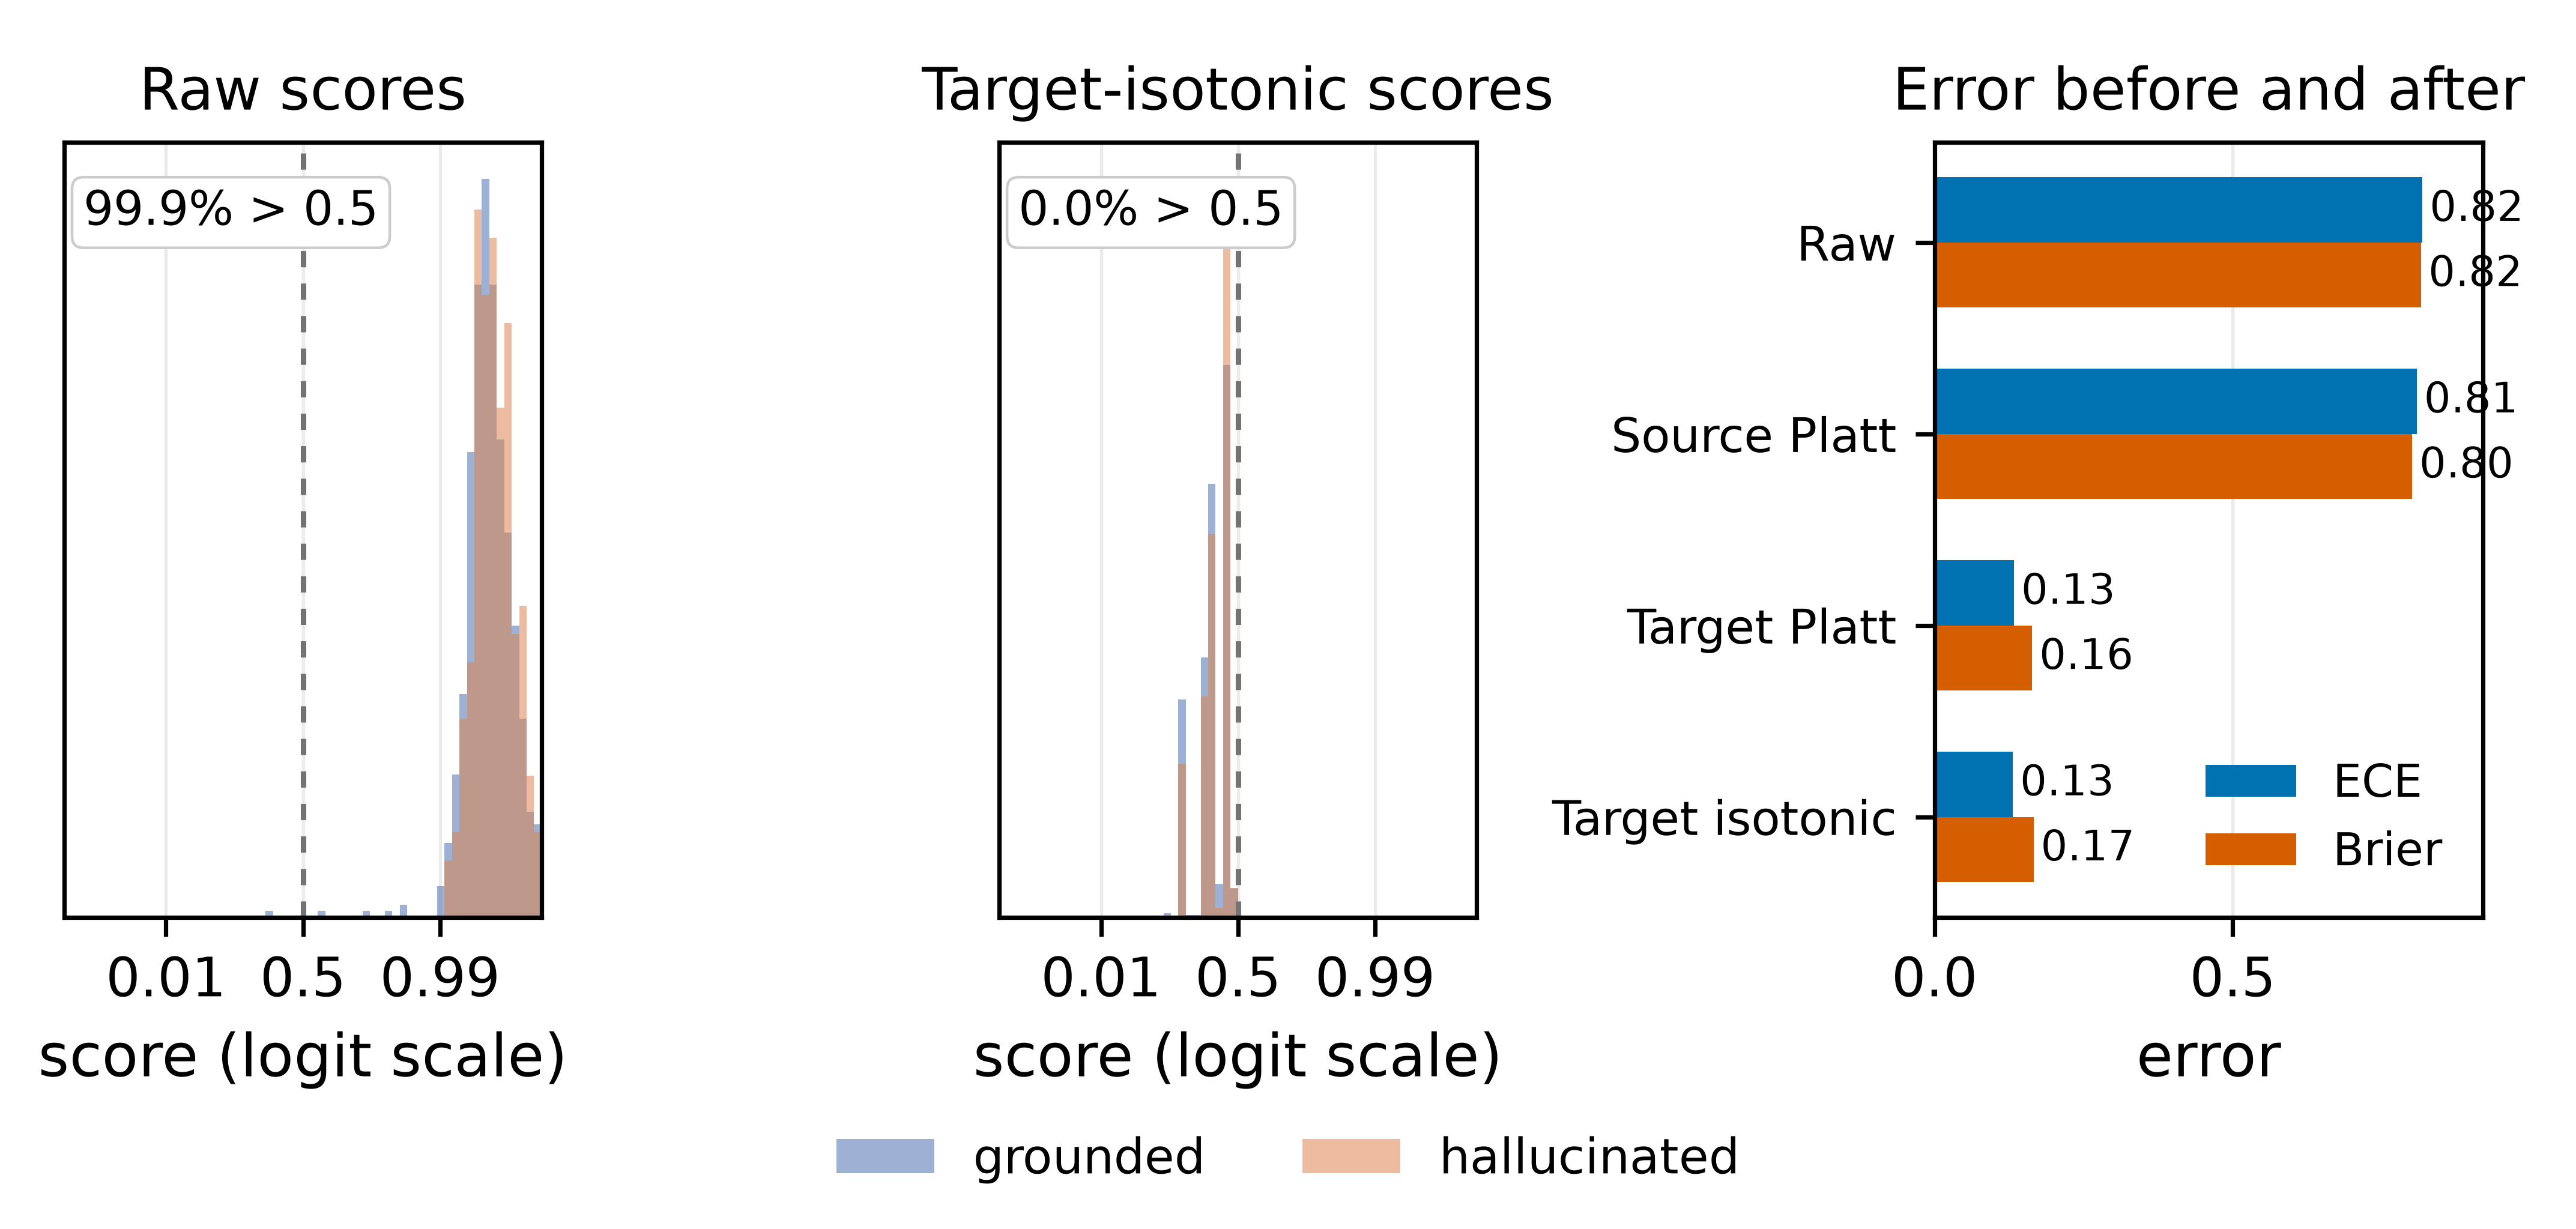
\includegraphics[width=\linewidth]{b4/calibration_shift.png}
  \caption{Target-domain recalibration of the conventional model on RAGTruth QA.}
  \label{fig:calibshift}
\end{figure}

Table~\ref{tab:conformal} reports the coverage. Within this framework, the nonconformity score for label $y$ is $s(x,y)=1-\hat{p}_y(x)$, where $\hat{p}_1=\hat{p}$ and $\hat{p}_0=1-\hat{p}$; thus, a coverage guarantee to the score is added by split conformal prediction, in actual application; in fact, the calibration quantile and the prediction set are
\begin{equation}
  \hat{q} = s_{(k)}, \quad k = \left\lceil (n+1)(1-\alpha) \right\rceil,
  \qquad
  C(x) = \{y : s(x,y) \le \hat{q}\},
  \label{eq:conformal}
\end{equation}
where $s_{(1)} \le \cdots \le s_{(n)}$ are the ordered calibration scores; this finite-sample order statistic yields coverage of at least $1-\alpha$ for the prediction set, and a class-conditional version is replacing the single quantile with one quantile per label,
\begin{equation}
  \hat{q}_y = s_{y,(k_y)}, \quad k_y = \left\lceil (n_y+1)(1-\alpha) \right\rceil,
  \qquad
  C(x) = \{y : s(x,y) \le \hat{q}_y\},
  \label{eq:conformal_class}
\end{equation}
where $s_{y,(1)} \le \cdots \le s_{y,(n_y)}$ are the ordered scores in class $y$ and $n_y$ is the number of calibration rows with label $y$, in many respects.
The principal run fits the Platt map and the quantile on the same 5{,}034 rows, so its coverage is a construction check; it is giving 0.940 and 0.967 coverage on QA and 0.900 and 0.950 on the calibration rows, on the whole. A disjoint sensitivity is fitting Platt on 2{,}514 rows and the quantile on 2{,}520 rows, to a significant degree. On that split, the 900 QA test rows are reaching 0.944 coverage at 90\%, so the minor guarantee holds. Against this backdrop, the insignificant guarantee hides the class split, like positive coverage is 0.685; while negative coverage is 1.000. Positive coverage is raised to 0.887 by a class-conditional quantile on the full calibration rows, still slightly below symbolic. FaithBench coverage falls to 0.320 and positive coverage to 0.003, because a Platt map fitted on QA is sending almost every FaithBench score to the negative side. Conformal prediction therefore certifies the slight rate only when the calibrator and the quantile are fitted on disjoint rows; it does not transfer, across the task shift. Multicalibration by answer length and claim count shows where the average ECE hides discrepancy, so on the 900 QA test rows, the target-Platt score has overall ECE 0.125. FaithBench is not sharpened by the QA calibrator, such as its target-Platt ECE is 0.629 against 0.453 for the raw score. The Brier score does not follow the ECE ranking, so the average is not a safe summary for short or one-claim answers. The worst length bin is 60 words or fewer (n=154), with ECE 0.275; the worst claim-count bin is a single claim (n=36), with ECE 0.346.

\begin{table}[pos=htbp]
  \centering
  \caption{Split and class-conditional conformal coverage on RAGTruth QA and FaithBench, mean over seeds 42/123/456. Class-conditional rows use the full 5{,}034 calibration rows; split rows use the disjoint halves.}
  \label{tab:conformal}
  \begin{tabular}{llrrrrr}
    \toprule
    \textbf{Dataset} & \textbf{Method} & $\alpha$ & \textbf{Coverage} & \textbf{Pos.} & \textbf{Neg.} & \textbf{Set size} \\
    \midrule
    QA test    & split       & 0.10 & 0.944 & 0.685 & 1.000 & 1.59 \\
    QA test    & split       & 0.05 & 0.972 & 0.842 & 1.000 & 1.75 \\
    QA test    & class-cond. & 0.10 & 0.886 & 0.887 & 0.886 & 1.69 \\
    QA test    & class-cond. & 0.05 & 0.936 & 0.925 & 0.938 & 1.80 \\
    FaithBench & split       & 0.10 & 0.320 & 0.003 & 1.000 & 1.00 \\
    FaithBench & split       & 0.05 & 0.323 & 0.006 & 1.000 & 1.01 \\
    \bottomrule
  \end{tabular}
\end{table}

\begin{figure}[pos=htbp]
  \centering
  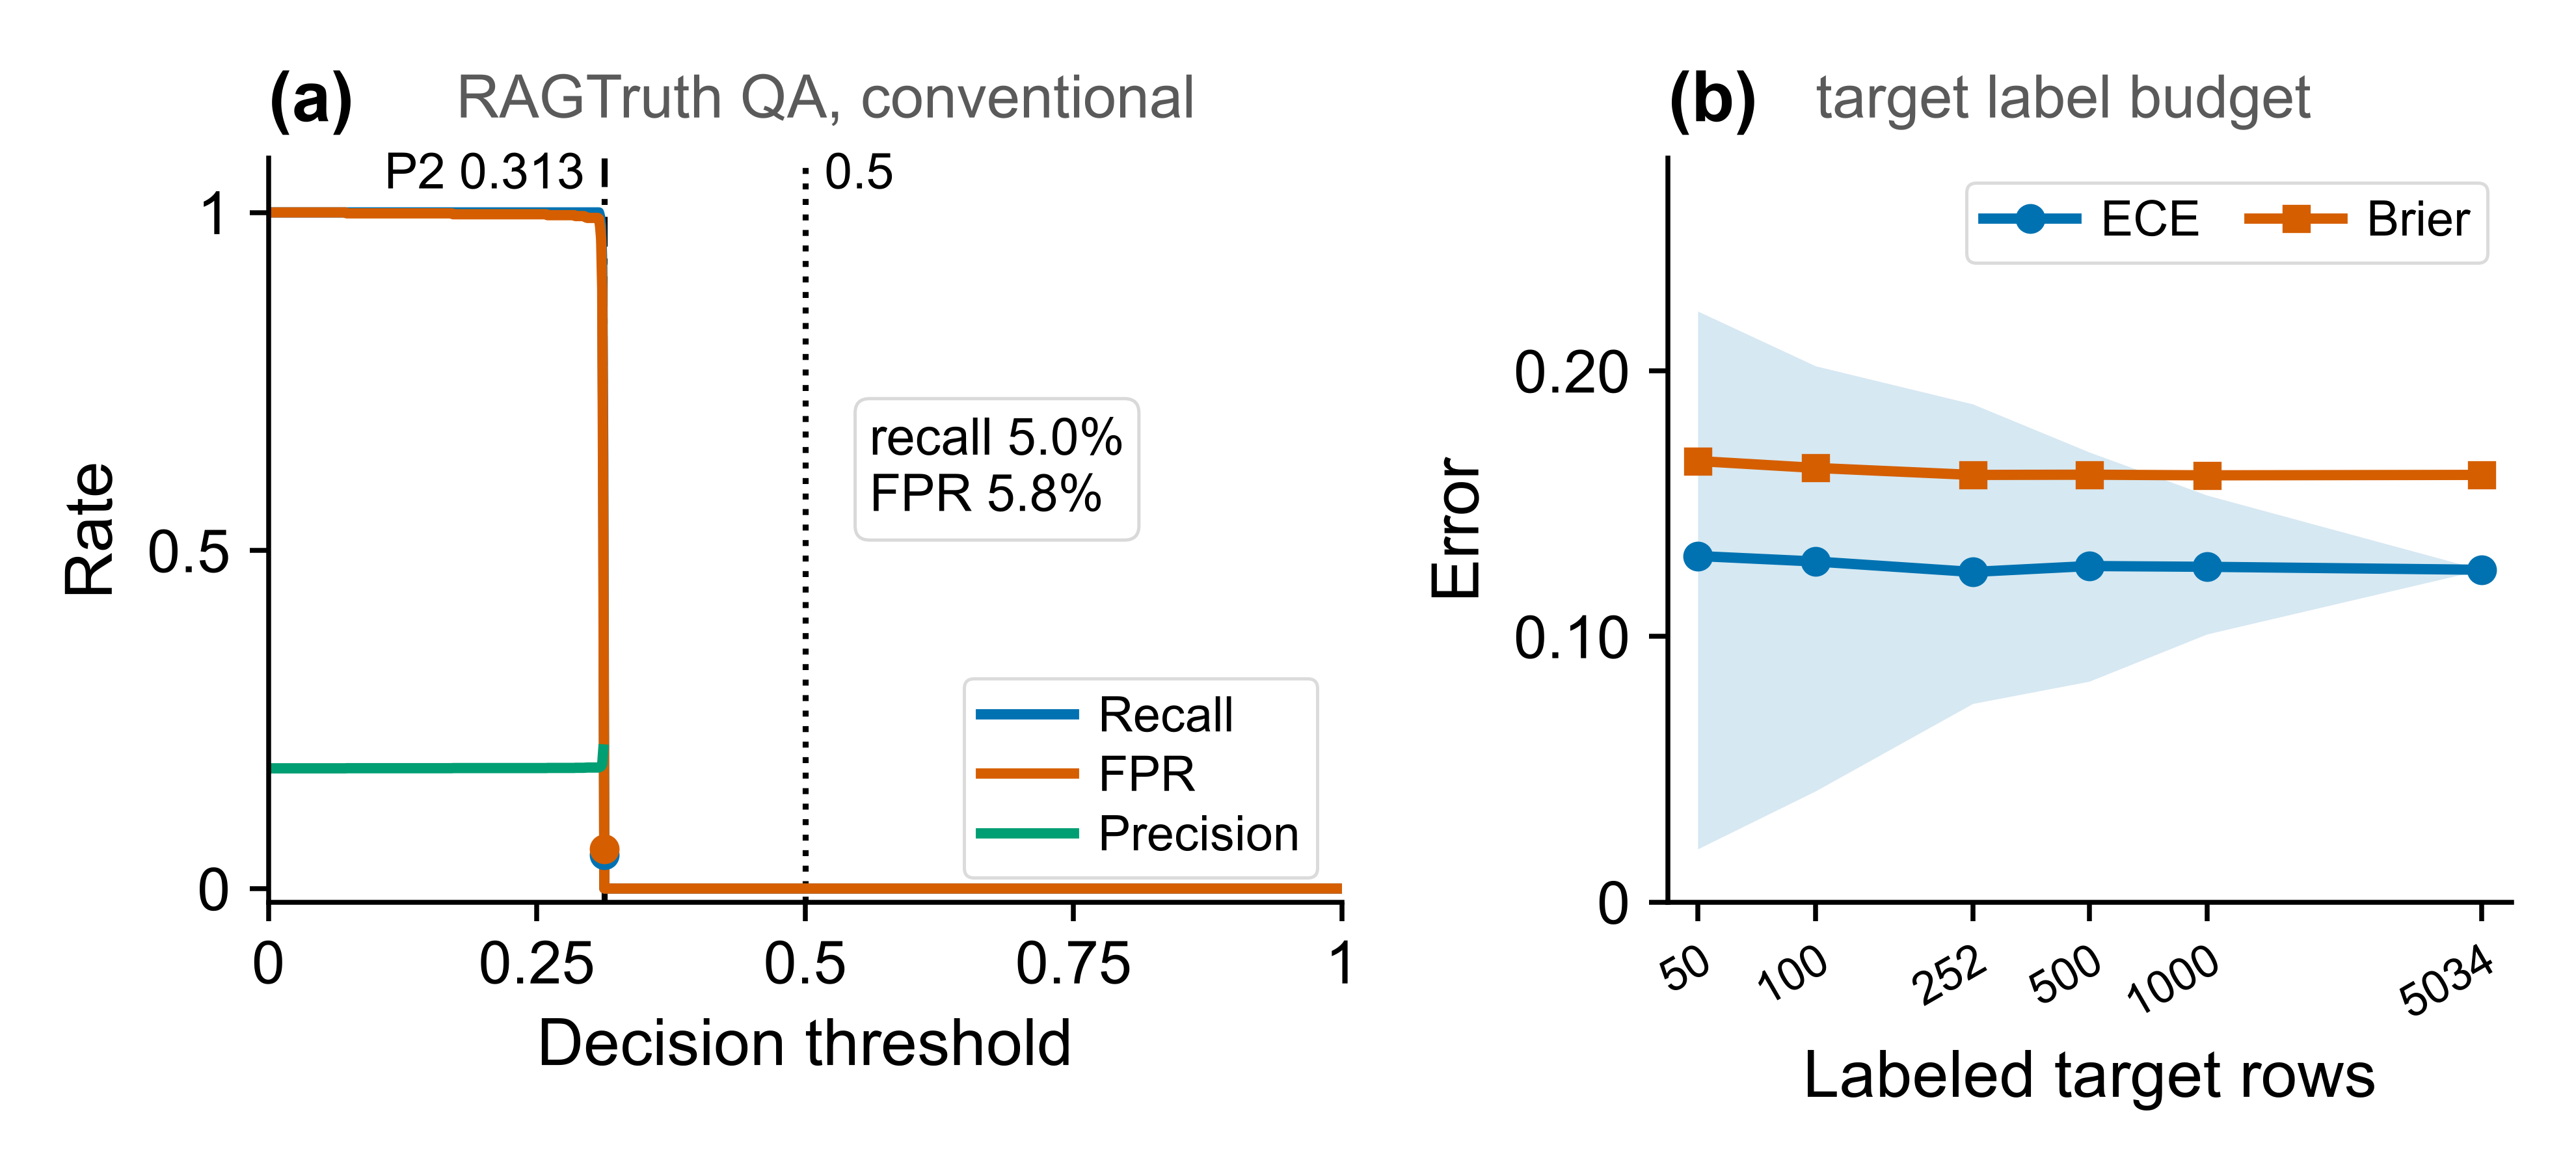
\includegraphics[width=\linewidth]{revision/operating_point_label_budget.png}
  \caption{Operating point for the conventional target-Platt model and 100-draw label budget for the fixed-hp m3 calibrator on RAGTruth QA.}
  \label{fig:operating}
\end{figure}

The standard reference m0 is trained only on HaluEval, and EC-XGB also sees RAGTruth summarization and data-to-text rows, so those two pairs measure adaptation, not broad shift (Table~\ref{tab:shift}), in many respects. Held-out QA is remaining near chance (AUROC 0.547 to 0.549); indeed, the gain is task-specific, namely summarization AUROC rises from 0.634 to 0.736 and data-to-text from 0.567 to 0.771, in many respects. On the pooled RAGTruth test split, the flag rate falls from 99.9\% to 61.3\% and AUROC rises from 0.475 to 0.582, and FaithBench AUROC rises from 0.509 to 0.594. Yet, f1 falls from 0.813 to 0.120 and raw ECE rises from 0.292 to 0.450, so the raw scores transfer poorly; in fact, the all-positive baseline is matched by the standard F1, because it flags almost every row. Under these conditions, eCE applies raw scores, F1 applies a fixed 0.5 threshold; and thus, also, flagged is the share above it. Tables~\ref{tab:ablation}, \ref{tab:target}, \ref{tab:external}, and \ref{tab:judge} report the fixed-hp refit; Table~\ref{tab:shift} reports the tuned B6 checkpoint.

\begin{table}[pos=htbp]
  \centering
  \caption{External and adaptation performance of B6 m0 and EC-XGB m3 from the tuned B6 run, mean over three seeds.}
  \label{tab:shift}
  \begin{tabular}{llccccc}
    \toprule
    \textbf{Dataset / task} & \textbf{Model} & \textbf{F1} & \textbf{AUROC} & \textbf{PR-AUC} & \textbf{Flagged} & \textbf{ECE} \\
    \midrule
    RAGTruth pooled         & Conventional (m0) & 0.5181      & 0.4753         & 0.3139          & 99.9\%           & 0.6346       \\
    RAGTruth pooled         & EC-XGB (m3)       & 0.5608      & 0.5815         & 0.3588          & 61.3\%           & 0.2782       \\
    \addlinespace
    RAGTruth QA             & Conventional (m0) & 0.3022      & 0.5465         & 0.1911          & 99.9\%           & 0.8149       \\
    RAGTruth QA             & EC-XGB (m3)       & 0.3081      & 0.5491         & 0.1884          & 97.4\%           & 0.7433       \\
    \addlinespace
    RAGTruth summarization  & Conventional (m0) & 0.3702      & 0.6343         & 0.3536          & 99.8\%           & 0.7499       \\
    RAGTruth summarization  & EC-XGB (m3)       & 0.3434      & 0.7358         & 0.4449          & 11.6\%           & 0.0519       \\
    \addlinespace
    RAGTruth data-to-text   & Conventional (m0) & 0.7830      & 0.5665         & 0.6831          & 100.0\%          & 0.3390       \\
    RAGTruth data-to-text   & EC-XGB (m3)       & 0.8234      & 0.7705         & 0.8374          & 74.9\%           & 0.0527       \\
    \addlinespace
    FaithBench              & Conventional (m0) & 0.8130      & 0.5089         & 0.6735          & 99.5\%           & 0.2917       \\
    FaithBench              & EC-XGB (m3)       & 0.1201      & 0.5941         & 0.7109          & 7.3\%            & 0.4500       \\
    \bottomrule
  \end{tabular}
\end{table}

The task-shift test is the weakest. On dialogue, 99.3\% of rows is flagged by m3. Also, its F1 equals the all-positive baseline, with AUROC 0.763; the length-only baseline is reaching 0.724, in actual application. From this perspective, still on summarization, m3 is reaching AUROC 0.717 and flags 37.5\%, which is why simultaneously, the length-only baseline reaches 0.788 and flags every row, in actual application. The standard m0 model flags 99.2\% of dialogue rows and 97.7\% of summarization rows, with AUROC 0.741 and 0.605. On dialogue, both models collapse to the all-positive baseline in F1. Also, nonetheless, their AUROCs stay above chance; on summarization, both rank below the length-only model. Simultaneously, the external panels pile both classes near 1.0, so the 0.5 threshold flags almost every row; this is the visual form of the 99.9\% flag rate in Table~\ref{tab:shift}. Figure~\ref{fig:transferscore} is revealing the raw score distributions of the standard model, such as the HaluEval panel is separating the classes.

\begin{table}[pos=htbp]
  \centering
  \caption{External validity on corpora never used for training, calibration, threshold selection, or model choice.}
  \label{tab:external}
  \begin{tabular}{llrrrrr}
    \toprule
    \textbf{Dataset (n)} & \textbf{Model} & \textbf{F1} & \textbf{AUROC} & \textbf{ECE} & \textbf{Flagged} & \textbf{Pair acc.} \\
    \midrule
    MedHallu (2{,}000) & EC-XGB (m3) & 0.667 & 0.821 & 0.493 & 100.0\% & 0.867 \\
                       & Conventional (m0) & 0.667 & 0.781 & 0.499 & 100.0\% & 0.822 \\
                       & Length-only & 0.667 & 0.260 & 0.500 & 100.0\% & 0.200 \\
    \addlinespace
    HaluBench (900)    & EC-XGB (m3) & 0.588 & 0.600 & 0.334 & 50.3\% & --- \\
                       & Conventional (m0) & 0.585 & 0.609 & 0.346 & 51.6\% & --- \\
                       & Length-only & 0.441 & 0.514 & 0.420 & 33.2\% & --- \\
    \addlinespace
    HaluEval dialogue (2{,}000) & EC-XGB (m3) & 0.670 & 0.763 & 0.488 & 99.3\% & --- \\
                       & Length-only & 0.680 & 0.724 & 0.438 & 95.9\% & --- \\
    \addlinespace
    HaluEval summarization (2{,}000) & EC-XGB (m3) & 0.583 & 0.717 & 0.113 & 37.5\% & --- \\
                       & Length-only & 0.667 & 0.788 & 0.500 & 100.0\% & --- \\
    \bottomrule
  \end{tabular}
\end{table}

Table~\ref{tab:external} reports the three external corpora and the task-shift pair. The fixed-hp m3 model ranks the paired hallucinated answer above the grounded answer in 86.7\% of 1{,}000 medical pairs [84.5, 88.7], with AUROC 0.821 [0.806, 0.837] on the 2{,}000 rows, to a significant degree; MedHallu is the strongest proof that the ranking survives a domain change and the clearest indication that the probability does not, in actual application. Against this backdrop, the pair accuracy over $M$ pairs is
\begin{equation}
  \mathrm{PA} = \frac{1}{M}\sum_{m=1}^{M}\mathbf{1}\left[\hat{p}(a_m^{+}) > \hat{p}(a_m^{-})\right],
  \label{eq:pair}
\end{equation}
where $a_m^{+}$ is the hallucinated answer and $a_m^{-}$ the grounded answer. 82.2\% and 0.781 are hit by the standard m0 model; in fact, the length-only baseline is inverted, at 20.0\% and 0.260, because grounded MedHallu answers are longer than the paired hallucinations (39.7 vs 27.8 words), the opposite of HaluEval (2.2 vs 11.0), broadly speaking. From this perspective, the ranking therefore transfers, but the scale does not - m3 flags every row, so its F1 is the all-positive 0.667 and its ECE is 0.493, broadly speaking; and thus, the source indicator is one for MedHallu and zero for HaluBench; a source-zero sensitivity on MedHallu changes pair precision by at most 0.003 and AUROC by at most 0.002, so the indicator does not drive the finding. HaluBench is a 30\% stratified sample. Its overall AUROC is 0.600, with covidQA 0.833, DROP 0.513, and FinanceBench 0.527; the model transfers to the biomedical subset but is at chance on the other two. All evaluation sets are balanced 50/50 by construction, so F1 and the flag rate are prevalence-dependent and do not outline natural rollout; HaluBench is unpaired, so pair precision is undefined, and the length-only baseline is fit once on HaluEval train only; in fact, the length-only baseline is at 0.514 overall, so 0.600 is not a length artifact.

\begin{figure}[pos=htbp]
  \centering
  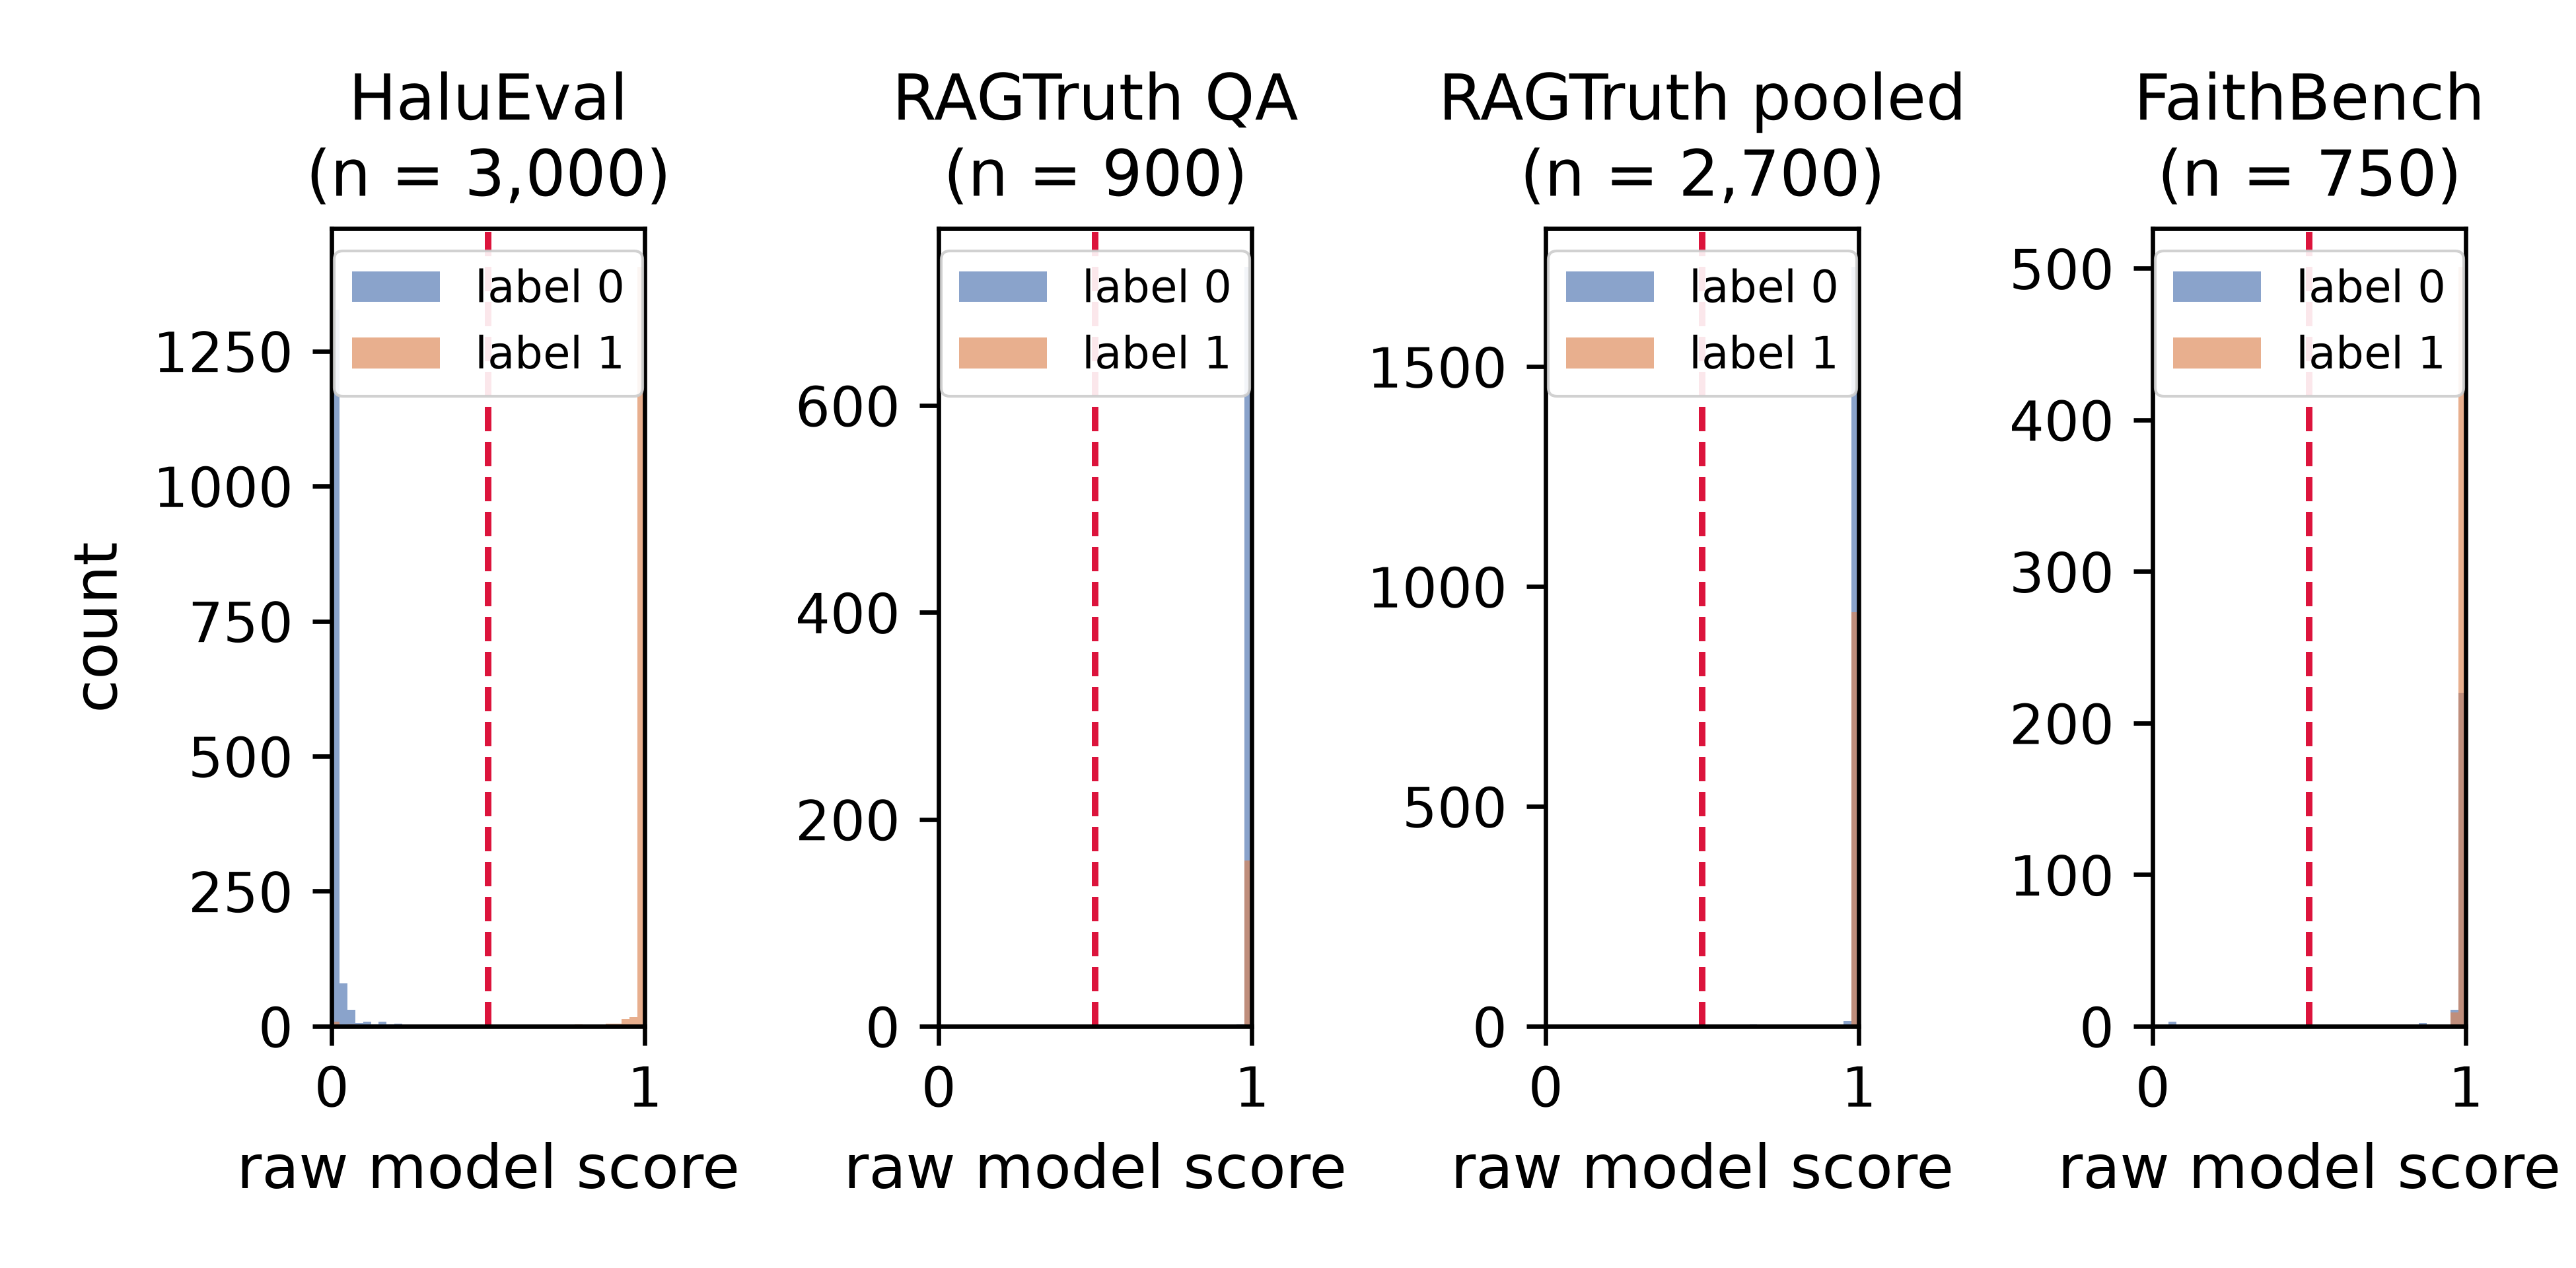
\includegraphics[width=\linewidth]{b3/transfer_score_distributions.png}
  \caption{Raw score distributions of the conventional B2 model on HaluEval and the external test rows.}
  \label{fig:transferscore}
\end{figure}

An index stress test is asking whether the weak held-out QA result is a retrieval problem, in real-world scenarios; and thus, replacing the gold setting with the top-5 retrieved passages changes AUROC from 0.545 to 0.521, F1 from 0.345 to 0.349, and ECE from 0.706 to 0.704, in many respects. On a 300-row, 50-group sample, recall@1 is 0.94, recall@5 and recall@10 are 1.00, and MRR is 0.959, and the 989 RAGTruth QA source documents are covered by the hybrid BM25 and FAISS index. From this perspective, the AUROC delta is $-$0.023 [$-0.061$, 0.011], which is encompassing zero; indeed, retrieval is therefore not the holdup - the model is near chance on RAGTruth QA even with the gold source passage. The qrels are the known source passage, not human web-search judgments, so this measures index recall, not end-to-end search quality; indeed, the sample has 50 source groups, so the interval is broad.

\subsection{Statistical Analysis}

Statistical tests apply the paired fixed-hyperparameter predictions and 2{,}000 two-level bootstrap draws, where groups are resampled within each seed and then seeds are resampled, in real-world scenarios; indeed, McNemar's test is comparing the clashing counts $b$ and $c$ on the paired seed-42 rows, where $b$ is the number of rows where the first model is right, broadly speaking. Also the second is wrong, and $c$ is the reverse; the statistic applies a continuity correction. Table~\ref{tab:mcnemar} is giving the McNemar counts. Before resampling seeds, the two-level version resamples groups within each seed. The 95\% interval is, to be sure, the 2.5th and 97.5th percentile of the paired bootstrap deltas; holm's technique controls the family-wise error rate across the four baseline comparisons. Across the three seeds, the Wilcoxon signed-rank test is comparing the two models; in fact, under the rolled out checkpoints ($p=0.45$), EC-XGB and the standard model are not markedly diverse. Also, the fixed-hyperparameter ablation is giving $p=0.789$ on the same test rows; indeed, the fixed-hp m0-vs-m3 comparison is the primary test. Also, it is not part of the Holm family, which is covering the four baseline comparisons against the standard model; and thus, the Wilcoxon test across the three seeds can't reach significance (minimum $p=0.25$). Against this backdrop, Table~\ref{tab:stats} reports the two-level bootstrap. Logistic regression and the heuristic are greatly worse ($p=1.86\times10^{-10}$ and $p=2.28\times10^{-30}$), and both survive Holm correction; in fact, the random forest is matching the standard model ($p=0.502$). The test is using the single configuration of Table~\ref{tab:ec}; On HaluEval, the m3$-$m0 F1 delta is $+$0.0006 [$-0.0010$, 0.0021], which is encompassing zero, and the AUROC delta is $+$0.0007 [0.0002, 0.0012], which is excluding zero by a small margin. The m2$-$m1 F1 delta is $-$0.0004 [$-0.0020$, 0.0012], and the m3$-$m1 delta is $+$0.0001 [$-0.0015$, 0.0018], so the claim features do not add an accumulate gain, and their AUROC deltas are $+$0.0009 and $+$0.0010, both with intervals above zero, so the added features reorder a few rows without changing F1.

On held-out RAGTruth QA the m3$-$m0 F1 delta is $+$0.0076 [0.0045, 0.0109], but the AUROC delta is $+$0.0017 [$-0.0270$, 0.0291], which is encompassing zero, in actual application; the paired fixed-minus-tuned contrasts all include zero, so the restore does not change all these conclusions, in actual application. On the pooled seen tasks the F1 delta is $+$0.0451 [0.0348, 0.0554] and the AUROC delta is $+$0.0962 [0.0644, 0.1295], which is the adaptation gain. From this perspective, haluEval groups are item pairs (1{,}500), RAGTruth QA has 150 source groups, and the pooled split has 450; the QA AUROC interval encompasses zero, so the held-out transfer result is not tackled, and the pooled row measures adaptation to seen task types, not unseen-task transfer; in fact, the F1 gain comes from flagging almost every row, not from better ranking.

\begin{table}[pos=htbp]
  \centering
  \caption{McNemar tests on the paired seed-42 HaluEval predictions.}
  \label{tab:mcnemar}
  \begin{tabular}{lrrrr}
    \toprule
    \textbf{Comparison} & \textbf{$b$} & \textbf{$c$} & \textbf{$p$} & \textbf{Holm $p$} \\
    \midrule
    EC-XGB vs conventional          & 10   & 6  & 0.453            & ---              \\
    EC-XGB vs conventional (fixed hp) & 8  & 6  & 0.789            & ---              \\
    Conventional vs random forest   & 12   & 8  & 0.502            & 0.502            \\
    Conventional vs logistic regression & 69 & 11 & $1.86\times10^{-10}$ & $3.7\times10^{-10}$ \\
    Conventional vs heuristic       & 158  & 9  & $2.28\times10^{-30}$ & $6.8\times10^{-30}$ \\
    Conventional vs NLI-only        & 1006 & 26 & $5.6\times10^{-204}$ & $2.2\times10^{-203}$ \\
    \bottomrule
  \end{tabular}
\end{table}



\begin{table}[pos=htbp]
  \centering
  \caption{Two-level bootstrap deltas for the fixed-hyperparameter ablation (2{,}000 draws; groups within seed, then seeds). Intervals are 95\%.}
  \label{tab:stats}
  \setlength{\tabcolsep}{4pt}
  \begin{tabular}{llcc}
    \toprule
    \textbf{Dataset} & \textbf{Comparison} & \textbf{$\Delta$F1 [95\% CI]} & \textbf{$\Delta$AUROC [95\% CI]} \\
    \midrule
    HaluEval          & m3$-$m0 & $+$0.0006 [$-0.0010$, 0.0021] & $+$0.0007 [0.0002, 0.0012] \\
    HaluEval          & m2$-$m1 & $-$0.0004 [$-0.0020$, 0.0012] & $+$0.0009 [0.0004, 0.0014] \\
    HaluEval          & m3$-$m1 & $+$0.0001 [$-0.0015$, 0.0018] & $+$0.0010 [0.0004, 0.0016] \\
    RAGTruth QA       & m3$-$m0 & $+$0.0076 [0.0045, 0.0109] & $+$0.0017 [$-0.0270$, 0.0291] \\
    RAGTruth pooled   & m3$-$m0 & $+$0.0451 [0.0348, 0.0554] & $+$0.0962 [0.0644, 0.1295] \\
    \bottomrule
  \end{tabular}
\end{table}

\subsection{Explanation, Efficiency, and Judges}

The fixed-hyperparameter m3 seed-42 checkpoint is used by the explanation results, and the top ten traits carry 77.9\% of the total attribution mass, and exact TreeSHAP reproduces the model margin to $9.2\times10^{-6}$, in real-world scenarios. Context overlap dominates, followed by word count, question-answer cosine, character count, and question-answer Jaccard; the claim-contradiction mean enters at rank eight, in many respects; in fact, the attributions are on the raw margin, not the display score. Figure~\ref{fig:shapimp} ranks the top-15 features by mean absolute SHAP over 1{,}000 stratified HaluEval test rows; in fact, the m3 ranking is agreeing with the frozen B2 ranking (Spearman $\rho=0.878$, Kendall $\tau=0.730$), so the claim attributes sharpen the explanation rather than replace the original drivers. Within this framework, cross-seed Spearman is 0.972 and 0.950, with nine of ten top characteristics shared and any equivalent top-5 set; the explanation is stable to the seed but less stable to content edits. Table~\ref{tab:perturb} uncovers the 20-case perturbation pilot: content edits move the score, structural edits barely are moving it, and the top-1 feature flips in 54.5\% of entity perturbations and none of the other operators; and thus, the entity flip rate is higher than in B2, so the explanation is less stable when the answer entity changes; per-operator $n$ is small. One more organized AI-assisted audit assessed 26 error-enriched cases picked, under B2 and re-scored under m3, with each explanation verified against the answer-context indication rather than the dataset label; and thus, thirteen explanations were judged unbelievable, three unsure. Also, ten tenable, so the explanations are diagnostic aids, not faithful attributions, and false positives inherit the length confound. Also, items from the setting are often reused by false negatives; in fact, because, the sample is error-enriched, the audit, not the test set is summarized by the percentages. The labels are author-checked pre-annotations - LLM tools helped the comment, so also, the authors reviewed and validated the final labels; agreement with the pre-annotations was 0.98 for explanation, 0.94 for taxonomy, and 0.88 for claims. Cohen's $\kappa$ was 0.965, 0.923, and 0.788; the authors changed 2\%, 6\%, and 12\% of rows; indeed, also the blind Fleiss $\kappa$ was 0.940, 0.868, and 0.761.

\begin{table}[pos=htbp]
  \centering
  \caption{Perturbation stability of the m3 raw score and SHAP ranking on HaluEval (seed 42, 20-case pilot).}
  \label{tab:perturb}
  \begin{tabular}{lcrrrr}
    \toprule
    \textbf{Operator}  & \textbf{n} & \textbf{$\Delta$score} & \textbf{Large rate} & \textbf{Top-1 flip} & \textbf{Spearman} \\
    \midrule
    Entity replacement & 11         & 0.339                  & 0.364               & 0.545               & 0.848             \\
    Support removal    & 10         & 0.464                  & 0.500               & 0.000               & 0.808             \\
    Number replacement & 3          & 0.332                  & 0.333               & 0.000               & 0.731             \\
    Date replacement   & 2          & 0.482                  & 0.500               & 0.000               & 0.786             \\
    \addlinespace
    Irrelevant insert  & 20         & 0.003                  & 0.000               & 0.000               & 0.922             \\
    Clause shuffle     & 2          & 0.000                  & 0.000               & 0.000               & 0.999             \\
    \bottomrule
  \end{tabular}
\end{table}

\begin{figure}[pos=ht]
  \centering
  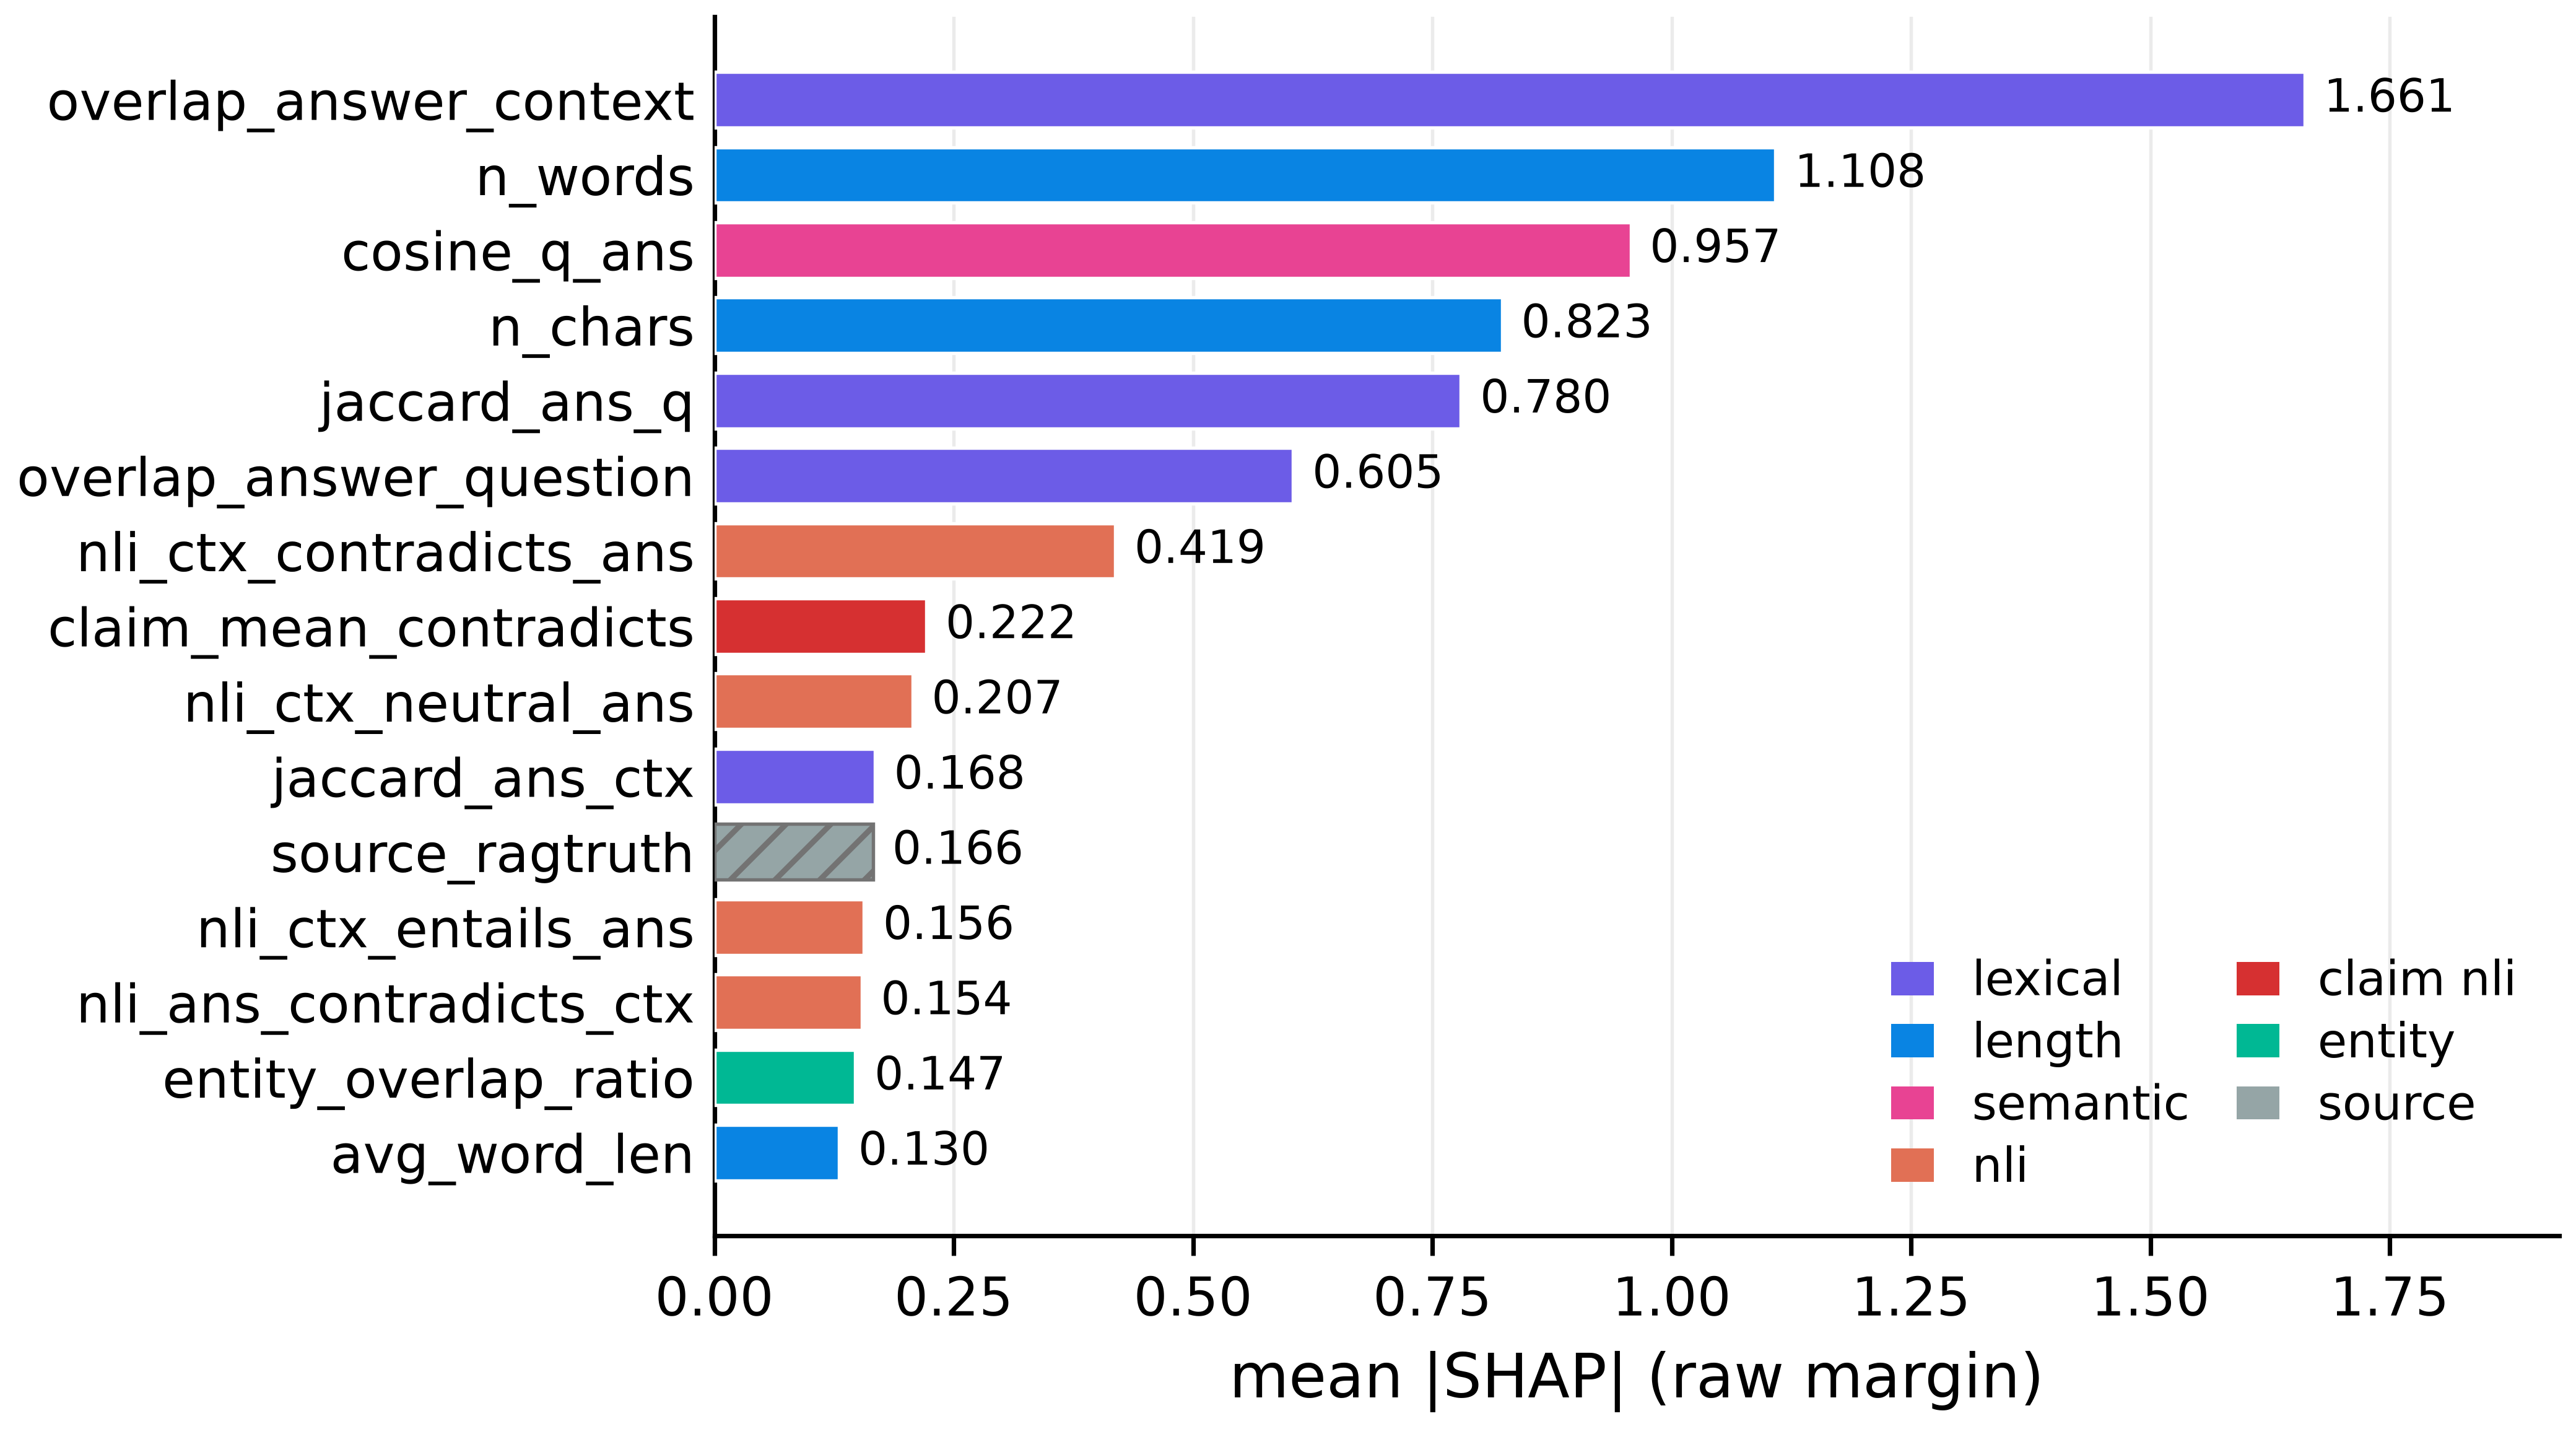
\includegraphics[width=\linewidth]{revision/m3_shap_summary.png}
  \caption{Mean absolute TreeSHAP for the fixed-hp m3 model (top 15 features).}
  \label{fig:shapimp}
\end{figure}

Table~\ref{tab:latency} gives the component latency. Constituents are timed in separate instrumented passes over the same samples, so they do not sum to the end-to-end median, and retrieval and judge calls are excluded, broadly speaking; and thus, while, XGBoost and SHAP are insignificant, NLI and NER dominate the base median. Adding the eight claim features raises the m3 path to 127.5~ms at the median, on the whole; indeed, the same 200-row protocol on CPU takes 2.00~s per answer in the single argued run (p50 0.98~s, p95 7.56~s), so this figure rests on GPU feature extraction. Also feature extraction, not the model, is the cost. Table~\ref{tab:cost} juxtaposes cost and latency, such as classic heads run in under one millisecond, and also the two judges are 18 to 24 times slower than the m3 pipeline; this encoder alone takes 6.97~ms per row at batch 8 and fp16, so the feature pipeline is about 18 times slower. Nonetheless, a fine-tuned classification head is being still needed by the encoder; and thus, also its training cost is not encompassed. Size is the seed-42 artifact on disk. Model-only m3 inference is 0.008~ms, and the NLI-only head is the NLI step plus a linear head. Recorded token counts and an presumed \$1.20/M output price are, put simply, being used by the cost; and thus, also the encoder timing is at 512 tokens, an upper bound for the 256-token baseline.

\begin{table}[pos=htbp]
  \centering
  \caption{Per-component latency in milliseconds (n = 200).}
  \label{tab:latency}
  \begin{tabular}{lrrr}
    \toprule
    \textbf{Component} & \textbf{p50} & \textbf{p95} & \textbf{mean} \\
    \midrule
    Core lexical       & 0.10         & 0.15         & 0.11          \\
    Entity (spaCy NER) & 21.13        & 47.24        & 25.34         \\
    NLI (2 directions) & 27.09        & 68.60        & 40.09         \\
    Semantic (MiniLM)  & 9.25         & 15.55        & 12.56         \\
    XGBoost inference  & 1.26         & 8.80         & 2.62          \\
    SHAP explanation   & 1.91         & 15.52        & 3.65          \\
    Base total         & 61.77        & ---          & ---           \\
    Claim NLI (m3)     & 43.75        & 83.21        & 53.11         \\
    Total m3           & 127.51       & 234.59       & 145.89        \\
    \bottomrule
  \end{tabular}
\end{table}

\begin{table}[pos=htbp]
  \centering
  \caption{Per-baseline cost and latency.}
  \label{tab:cost}
  \begin{tabular}{llrrr}
    \toprule
    \textbf{Baseline}      & \textbf{Inputs} & \textbf{Size} & \textbf{p50 (ms)} & \textbf{Cost/1K} \\
    \midrule
    Heuristic (overlap)    & text            & ---           & 0.009                   & $\approx$\$0     \\
    Logistic regression    & 26 feats        & 1.1\,KB       & 0.001                   & $\approx$\$0.001 \\
    Random forest          & 26 feats        & 8.4\,MB       & 0.331                   & $\approx$\$0.001 \\
    NLI-only               & 6 NLI probs     & ---           & ---                     & $\approx$\$0.001 \\
    TF-IDF (answer/full)   & text            & 0.58/4.1\,MB  & 0.014/0.110$^\ast$      & $\approx$\$0.001 \\
    XGBoost (conventional) & 26 feats        & 0.49\,MB      & 0.005                   & $\approx$\$0.001 \\
    RoBERTa-base           & 512 tokens (timing) & 125M params & 6.97                  & training only    \\
    EC-XGB (m3)            & 35 feats        & 0.68\,MB      & 127.51                  & $\approx$\$0.001 \\
    GPT 5.6 Luna judge     & API             & ---           & 2283.07                 & \$0.234          \\
    Qwen 3.5 4B judge      & 4-bit local     & 4B params     & 3049.96                 & \$0              \\
    \bottomrule
  \end{tabular}
\end{table}

LLM judges are not fair evaluators. Taken together, also, their preferences can shift with answer order \cite{wang2024fair}. Table~\ref{tab:judge} is comparing EC-XGB with two judges on the RAGTruth QA rows at natural prevalence, in many respects. GPT-5.6 Luna is reaching AUROC 0.910 against 0.558 for EC-XGB; indeed, also, qwen 3.5 4B also outperforms it, so both judges are better QA detectors and the feature model's merit is cost, in many respects. The target-fitted length-only baseline also ranks the QA rows better than the full feature model; the paired interval for GPT minus EC-XGB is $-$0.052 [$-0.127$, 0.024], and the AUROC interval is $+$0.008 [$-0.034$, 0.048]. The length-matched panel changes the ranking: on the exact-length set, EC-XGB matches the stronger judge on AUROC and directs on F1, so the natural-prevalence gap is a domain-shift finding rather than a length effect; in fact, under matched multi-source training, the tailored encoder reaches 0.694 on the pooled RAGTruth test set, above EC-XGB's 0.582, so the encoder is stronger there. Still both are near chance. The feature model is less degraded on unseen tasks. Both include zero. Simultaneously, qwen is a single deterministic run, so the judge ranking is not stable. GPT applies default decoding and three seeds. GPT's F1 is moved from 0.814 to 0.854, across the three prompts by prompt choice, about the size of the model gap.

\begin{table}[pos=htbp]
  \centering
  \caption{Judge stress tests on the 900 RAGTruth QA rows and the 158-row length-matched HaluEval set.}
  \label{tab:judge}
  \setlength{\tabcolsep}{4pt}
  \begin{tabular}{lrrrrrrr}
    \toprule
    \textbf{Model}     & \textbf{P} & \textbf{R} & \textbf{F1} & \textbf{AUROC} & \textbf{Flagged} & \textbf{p50 (ms)} & \textbf{Cost/1K} \\
    \midrule
    GPT 5.6 Luna judge & 0.404      & 0.942      & 0.565       & 0.910          & 41.4\%           & 2283              & \$0.234          \\
    Qwen 3.5 4B judge  & 0.570      & 0.638      & 0.602       & 0.778          & 19.9\%           & 3050              & \$0              \\
    EC-XGB (m3)        & 0.183      & 0.998      & 0.310       & 0.558          & 96.8\%           & 127.5             & $\approx$\$0.001 \\
    Length-only        & 0.439      & 0.181      & 0.257       & 0.712          & 7.3\%            & ---               & $\approx$\$0 \\
    All-positive       & 0.178      & 1.000      & 0.302       & ---            & 100.0\%          & ---               & $\approx$\$0     \\
    \addlinespace
    \multicolumn{8}{l}{\emph{Length-matched HaluEval, 158 rows, 50\% positive}} \\
    GPT 5.6 Luna judge & 0.945      & 0.798      & 0.865       & 0.957          & 42.2\%           & 2283              & \$0.234          \\
    Qwen 3.5 4B judge  & 1.000      & 0.696      & 0.821       & 0.863          & 34.8\%           & 3050              & \$0              \\
    EC-XGB (m3)        & 0.954      & 0.865      & 0.907       & 0.956          & 45.4\%           & 127.5             & $\approx$\$0.001 \\
    Length-only        & 0.515      & 0.443      & 0.476       & 0.521          & 43.0\%           & ---               & $\approx$\$0     \\
    \bottomrule
  \end{tabular}
\end{table}

\subsection{Error Analysis and Discussion}

On the seed-42 fixed-hyperparameter run, m3 is making 43 deviations on the HaluEval test set (Figure~\ref{fig:confusion}), an error rate of 1.4\%, in real-world scenarios; the WP5 audit is covering seven of the eight false positives and 12 of the 35 false negatives, chosen to cover the codebook, broadly speaking. A separate 50-case sheet, reviewed by one author, adds 31 artifact cases and 19 content cases, across 12 categories; all these are describing the reviewed cases, not the 3{,}000-row test population. In this broader context, Table~\ref{tab:length} is revealing that length is a near-perfect label indicator on HaluEval, with false positives stronged in the five-to-eight bin and false negatives in the short bins, yet the 17+ bin negatively rows. Six length bins are equalized with 247 examples each by a reweighting control, so also, a length-matching control is pairing one positive and one negative at each individual length; indeed, reweighting is giving EC-XGB a gain of 0.039 F1 and 0.023 AUROC over the length-only regression, which is already competitive on its own (Table~\ref{tab:models}). 79 pairs (158 examples) over 1{,}000 bootstraps are given by length matching; in turn, EC-XGB is holding AUROC 0.956, and in two ways, the length distribution is changed by the controls, which is why in the interim, the length-only baseline falls to 0.521. The AUROC point gap is 0.435 (bootstrap mean 0.436 [0.351, 0.522]), and the F1 point gap is 0.431 (bootstrap mean 0.440 [0.334, 0.552]).

\begin{figure}[pos=htbp]
  \centering
  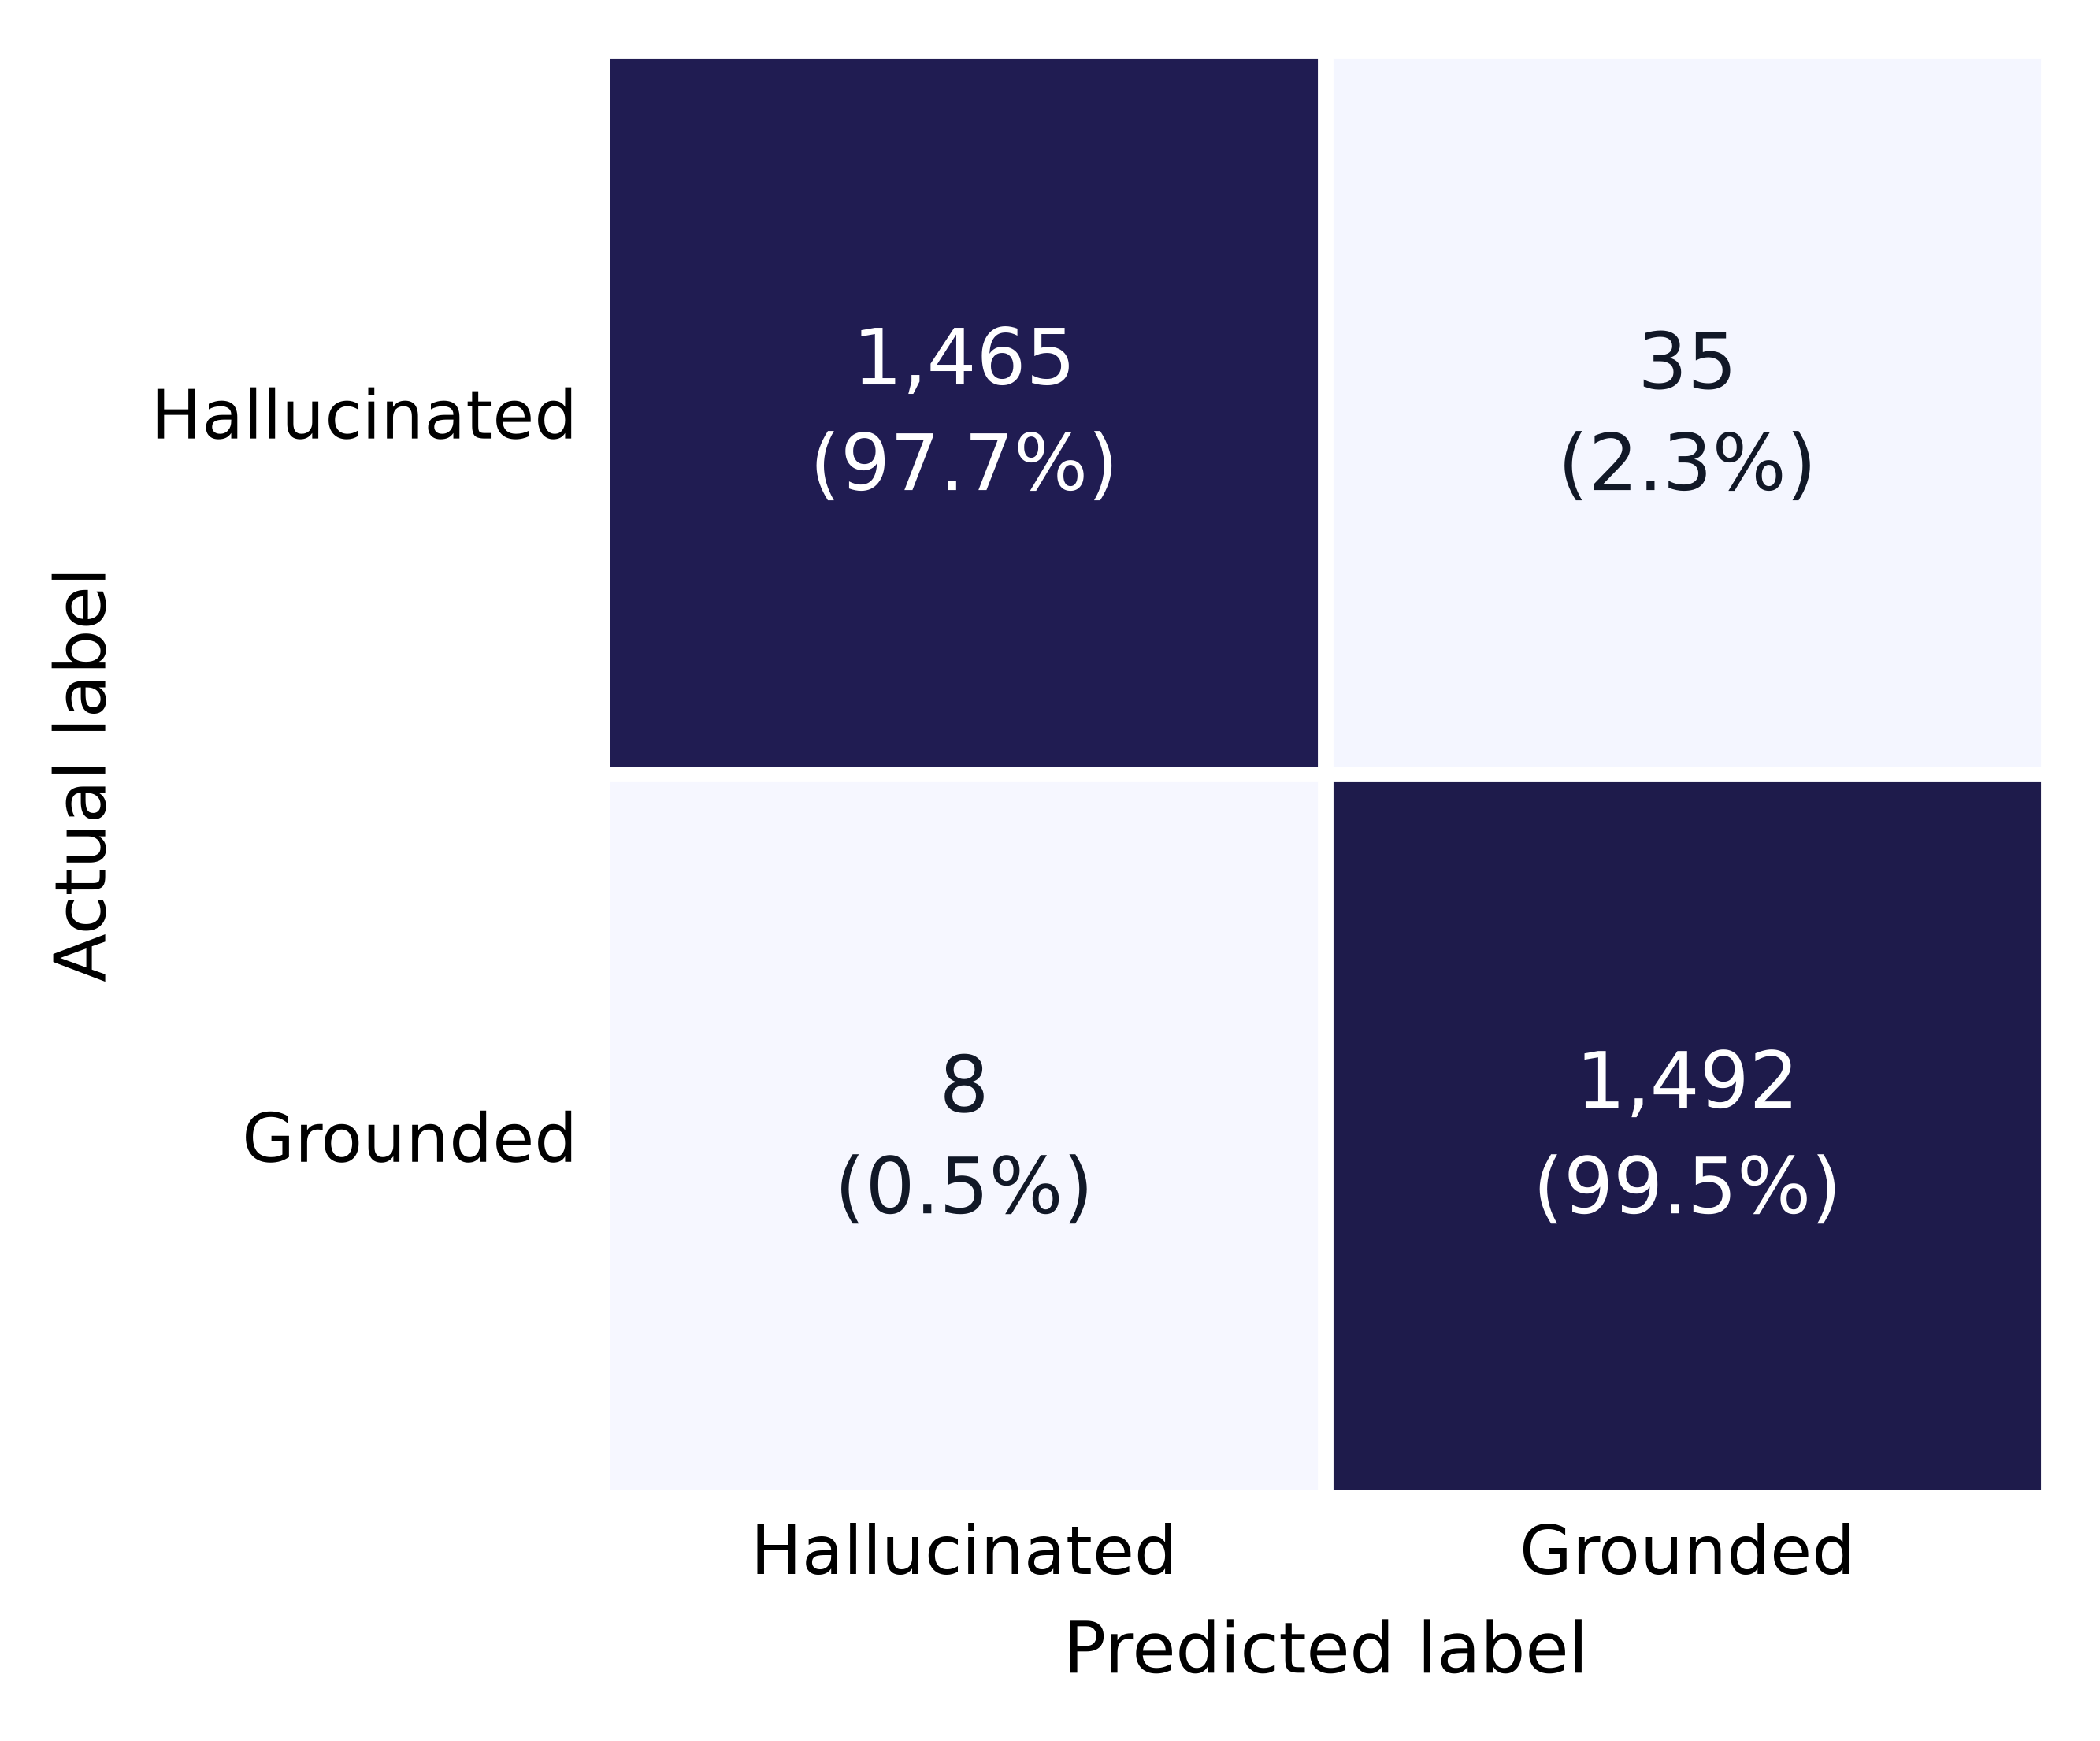
\includegraphics[width=0.62\linewidth]{revision/confusion_matrix.png}
  \caption{Confusion matrix for the seed-42 fixed-hp m3 model on the HaluEval test set at the 0.5 threshold (n = 3{,}000). Cell values are counts, with row-normalized percentages in parentheses.}
  \label{fig:confusion}
\end{figure}

\begin{table}[pos=htbp]
  \centering
  \caption{HaluEval test errors of the conventional B2 model by answer length (counts seed 42, rates three-seed means).}
  \label{tab:length}
  \begin{tabular}{lrrrrr}
    \toprule
    \textbf{Words} & \textbf{Rows} & \textbf{Hallucinated rate} & \textbf{FP rate} & \textbf{FN rate} & \textbf{Mean score} \\
    \midrule
    1              & 524           & 0.021                 & 0.004            & 0.182            & 0.024               \\
    2              & 514           & 0.033                 & 0.000            & 0.176            & 0.035               \\
    3--4           & 474           & 0.127                 & 0.002            & 0.178            & 0.126               \\
    5--8           & 641           & 0.902                 & 0.106            & 0.031            & 0.888               \\
    9--16          & 600           & 0.982                 & 0.000            & 0.003            & 0.980               \\
    17+            & 247           & 0.992                 & 0.333            & 0.000            & 0.993               \\
    \bottomrule
  \end{tabular}
\end{table}

\begin{figure}[pos=htbp]
  \centering
  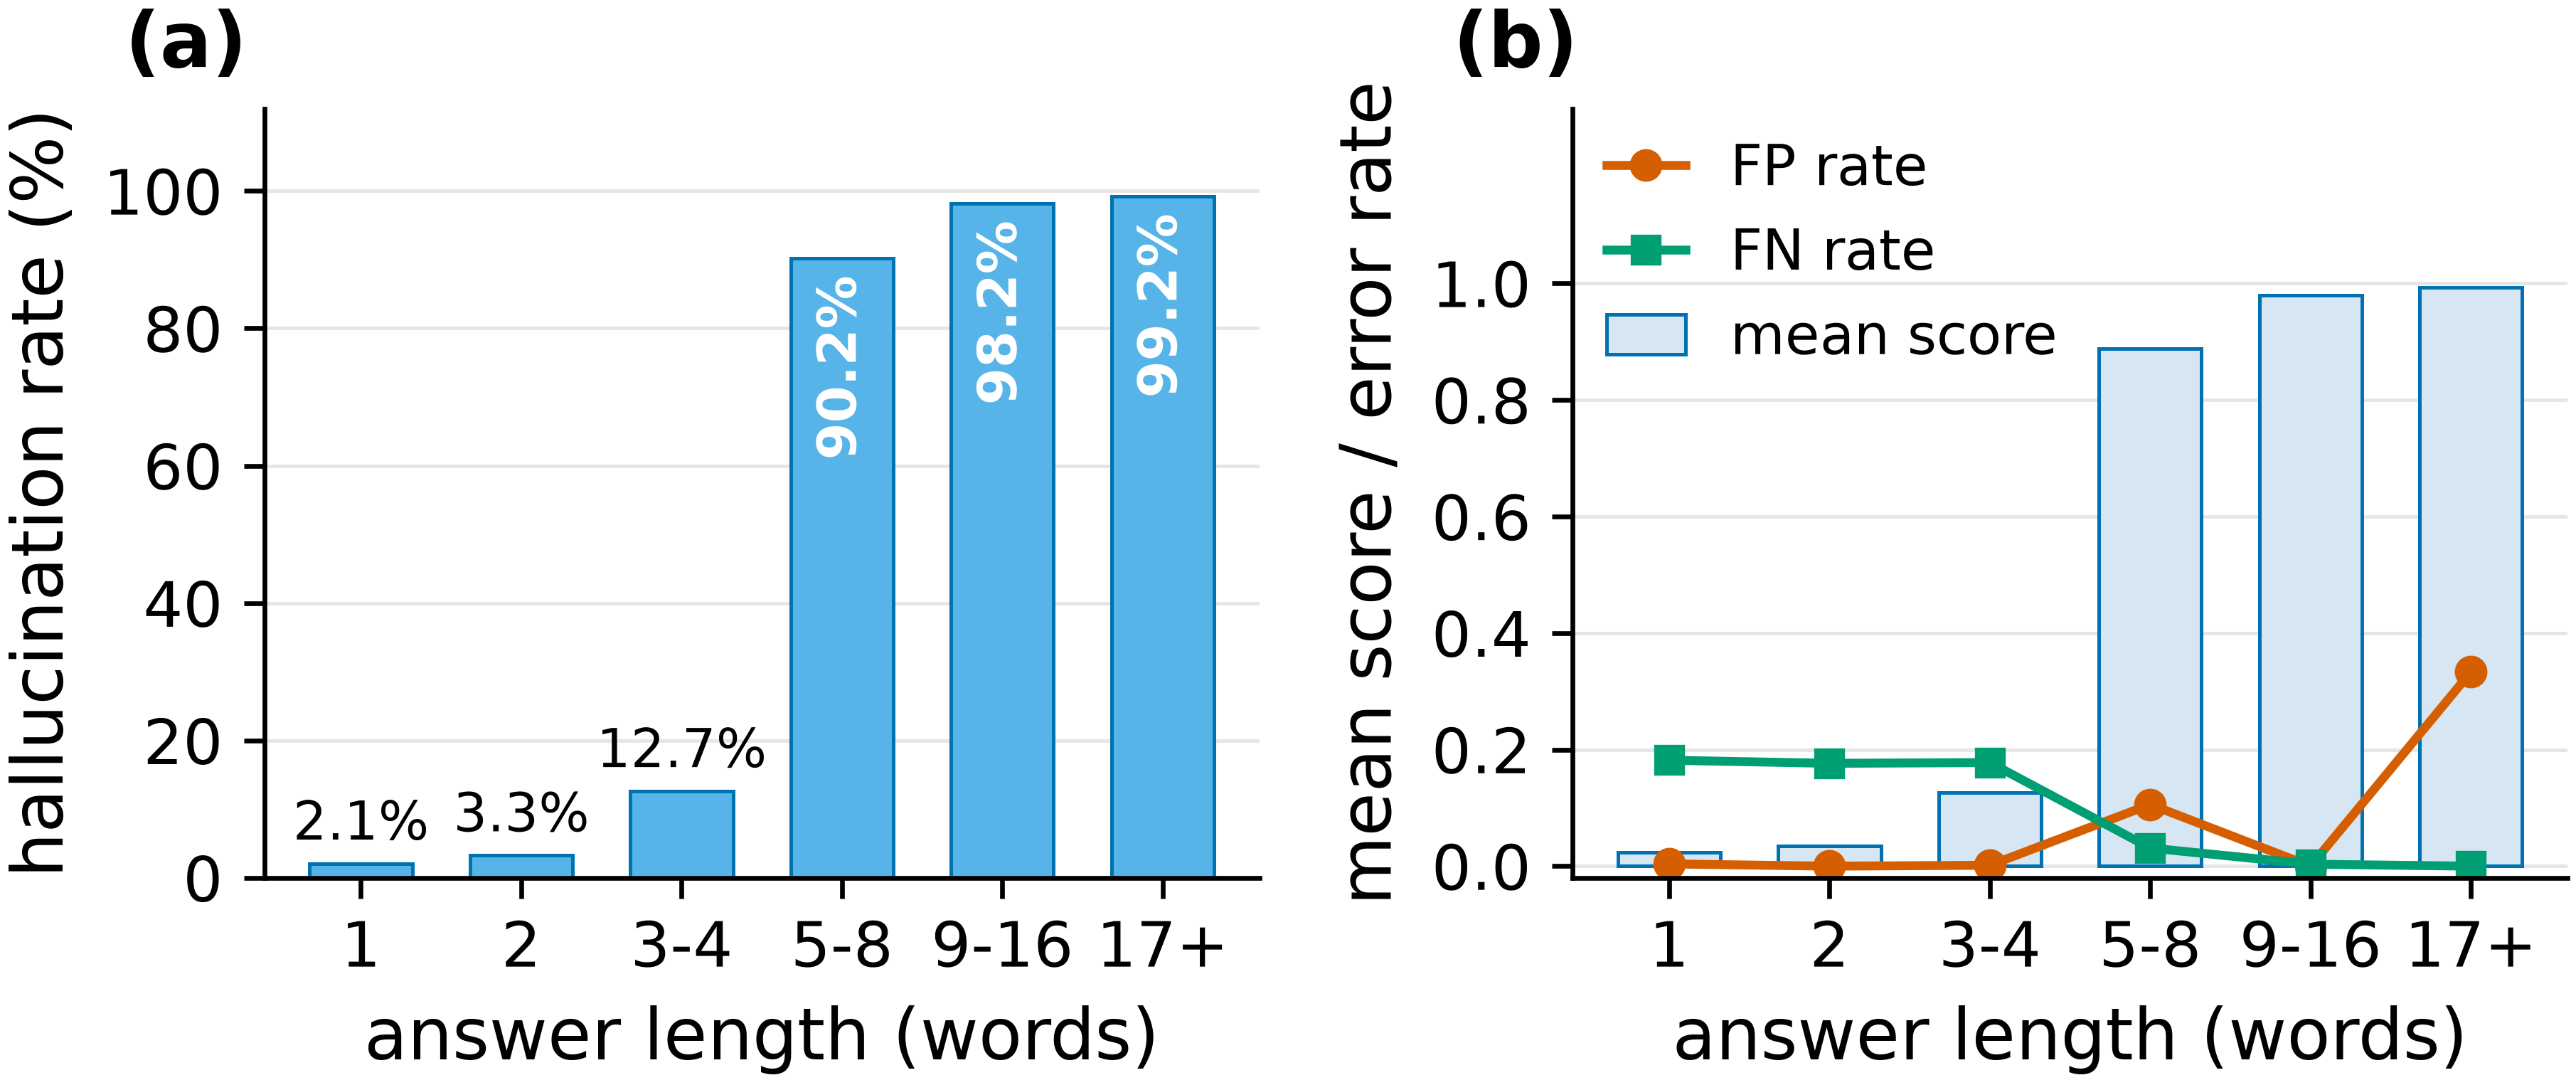
\includegraphics[width=\linewidth]{revision/length_analysis.png}
  \caption{Hallucination rate, mean score, and error rates by answer length for the B2 conventional model.}
  \label{fig:length}
\end{figure}

Figure~\ref{fig:length} reveals the same pattern. Complete sentences are long, so the standard model reads them as hallucinations; in turn, also, the in-domain model is mostly the length and overlap detector, in many respects; indeed, distinct splits, supervision and evidence access are implemented by Published HaluEval QA results. One supervised 13B agent reports F1 0.724 on 100 rows, so these published numbers are context rather than any head-to-head bar, broadly speaking, and the benchmark also is, to a large extent, asking for hallucinated answers about five words longer. Also the gathered gap is 8.5 words. Still semantic detection is exaggerated by any comparison that is ignoring this construction artifact; indeed, the claims in this inquiry are, for all practical purposes, bounded by the tests that were not run. Retrieval quality and end-to-end verdict accuracy are not assessed, this judge comparison controls length but not area, and the audit is error-enriched; the rolled out display calibrator was, to be sure, picked in one more earlier fit that juxtaposed Platt and isotonic on the test split. Also Table~\ref{tab:target} refits Platt without that selection.

\section{Conclusion}\label{sec:conclusion}

The present examination tested EC-XGB, a 35-trait evidence-consistent model, as a hallucination risk score and asked how its calibration and ranking change, under the area and task shift, broadly speaking; in fact, its ranking survives a change of corpus, so the score can (to some degree) order answers for review, in many respects. Also the per-claim verdicts give a reviewer a reason for each individual flag, which is why its probability does not survive that change - the display score needs labeled target rows, and also, the target prevalence then sets its level, so EC-XGB is therefore a domain-specific screening score, not a general-purpose detector. The next test is adaptation to an unseen QA domain, with thresholds chosen, under the prevalence shift; a seen-task source ablation would then separate the RAGTruth rows from the source indicator.

\printcredits

\section*{Declarations}
\begin{itemize}
  \setlength{\itemsep}{0pt}
  \setlength{\parsep}{0pt}
  \item \textbf{Funding:} No external funding was, in this setting, received by the current study.

  \item \textbf{Conflicts of Interest:} The authors are declaring that they knownly interest or personal relationships that could (in actual operation) have appeared to impact the work reported in this inquiry, in real-world scenarios.

  \item \textbf{Data availability:} Full raw datasets are not redistributed. RAGTruth (MIT) for HaluEval (MIT), and FaithBench (CC BY-NC-SA 4.0), the store is encompassing download scripts and a tracked license manifest with the source revisions and SHA-256 hashes, together with a 26-case audit file with benchmark excerpts. Model artifacts and the experiment manifest are, in essence, available from the related author on reasonable request. Splits and feature matrices can be reproduced from the original dataset sources. MedHallu (MIT) and the HaluBench subset (CC BY-NC 2.0) were determined from their formal releases.

  \item \textbf{Code availability:} The training pipeline, FastAPI inference service, and Next.js dashboard are generally available at \url{https://github.com/Atik203/HaluRISC} (branch \texttt{main}), to a significant degree; in fact, the code is, in practice, released under the MIT license.

  \item \textbf{Ethical approval:} No human-subject data were, in practice, collected. The authors inspected LLM-assisted pre-annotations of public benchmark rows for internal verification; in turn arguably, this does not constitute human-subjects research, so ethics approval was not needed, to a significant degree.
\end{itemize}


\section*{Acknowledgements}
The authors thank the maintainers of HaluEval, RAGTruth, FaithBench, MedHallu and HaluBench for releasing their datasets under the licenses that permit research use, in many respects; FaithBench is, put simply, released under CC BY-NC-SA 4.0 and HaluBench under CC BY-NC 2.0.

\hbadness=10000
\sloppy
\setlength{\bibsep}{0pt}
\renewcommand{\bibfont}{\fontsize{8.5pt}{9pt}\selectfont}
\bibliographystyle{elsarticle-num}
\bibliography{ref}

\vspace{4pt}
\end{document}
